\documentclass[12pt,a4paper]{article}
\usepackage[polish]{babel}
\usepackage{graphicx}
\usepackage[margin=2cm]{geometry}
\usepackage[T1]{fontenc}
\usepackage{hyperref}
\usepackage{url}
\usepackage[]{algorithm2e}
\usepackage{listings}
\usepackage[noend]{algpseudocode}
\usepackage{tikz}
\usepackage[utf8]{inputenc}
\usepackage{lmodern}
\usepackage{minted}
\usepackage{lipsum}
\usepackage{array}
\usepackage{longtable}

\usetikzlibrary{positioning}
\selectlanguage{polish}

\begin{document}
\clearpage

\begin{figure}[h]
\centering

\includegraphics[width=0.25\textwidth]{images/ps-logo.png}
\end{figure}

\begin{center}
\large{Wydział Matematyki Stosowanej}
\end{center}
\begin{center}
\large{Kierunek Informatyka}
\end{center}
\begin{center}
\large{Studia stacjonarne I stopnia}
\end{center}

\hspace{6cm}

\begin{center}
\Huge\textbf{Projekt Inżynierski}
\end{center}
\begin{center}
\Large{Gra sieciowa w środowisku aplikacji webowej - Szachy}
\end{center}

\hspace{6cm}
\\\\


\begin{minipage}[t]{0.3\textwidth}
    \begin{center}
    \normalsize{\textbf{Kierujący projektem:}\\dr inż. Zdzisław Sroczyński}
    \end{center}
\end{minipage}
\hfill
\begin{minipage}[t]{0.3\textwidth}
    \begin{center}
    \normalsize{\textbf{Autor:}\\Bruno Masłoń}
    \end{center}
\end{minipage}

\vfill

\begin{center}
Gliwice, 2025
\end{center}

\newpage

\pagenumbering{arabic}
\tableofcontents

\newpage

\section{Wstęp}
\subsection{Opis projektu - streszczenie}
    

Projekt BRNChess to aplikacja webowa, składająca się z dwóch głównych elementów - aplikacji internetowej (frontend), stworzonej w oparciu o technologie React + Vite, pisana w języku typescript oraz aplikacji serwerowej (backend), zbudowanej na platformie .NET Framework. 
\\

Aplikacja ta ma na celu umożliwienie użytkownikom rozgrywkę w jedną z najpopularniejszych gier pvp na świecie, jaką są szachy. Szachy to gra planszowa dla dwóch graczy, z których każdy kontroluje zestaw figur szachowych, a celem jest zaszachowanie króla przeciwnika, tj. zagrożenie mu nieuchronnym schwytaniem. Zasady gry w szachy, które są znane dzisiaj, pojawiły się w Europie pod koniec XV wieku, a ich standaryzacja i powszechna akceptacja nastąpiła pod koniec XIX wieku. Aplikacja umożliwia na rozegranie partii online wraz z innymi użytkownikami z całego świata jak na rozegranie meczu przeciwko silnikowi szachowemu. Dzięki dotnetowej paczce SignalR gra może toczyć się w czasie rzeczywistym przez co możliwe jest wykorzystanie kontroli czasowej podczas przebiegu partii, co wspiera częstsze odwiedziny strony internetowej.

\subsection{Główne założenia i cele projektu}

\begin{itemize}
    \item \textbf{Gra online:} Stworzenie aplikacji do gry w szachy online, jest głównym założeniem projektu. Gracze zostają dobierani w sposób losowy, w oparciu o ich obecną punktację.
    \item \textbf{Gra offline:} Integracja z opensourceowym projektem silnika szachowego "Stockfish", w celu umożliwienia użytkownikom gry z komputerem.
    \item \textbf{Gra ze znajomymi} Utworzenie systemu relacji pomiędzy użytkownikami, aby użytkowcy mogli rozgrywać partie ze swoimi znajomymi oraz w celu umożliwiania tworzenia własnych gier, niebędących przypadkowym wyborem.
    \item \textbf{Interfejs} Bardzo ważnym elementem współczesnych aplikacji jest interfejs użytkownika. Cały UI powinien być intuicyjny oraz przyjemny dla oka. Dobrane odpowiedniej stylistyki strony jak i jej poszczególnych elementów jest kluczowe, aby użytkowcy chętnie wybierali odwiedzali platforme.
    \item \textbf{Konto użytkownika} Zaprojektowanie kąt użytkowników, na których przechowywane będą wszystkie i dane, aktywności jak i osiągnięcia zdobywane podczas użytkowania aplikacji.
    \item \textbf{Bezpieczeństwo danych} Dane przekazywane przez użytkowników, powinny być przechowywane w sposób bezpieczny, w szczelności dane wrażliwe.
    \item \textbf{Hosting}
    \item \textbf{Dodatkowe funkcjonalności} Do dodatkowych funkcjonalności można zaliczyć między innymi: globalny ranking graczy jak i wśród znajomych, przegląd gier użytkownika, czy personalizacje konta i ustawień gry.
\end{itemize}

\newpage

\section{Stos technologiczny}
\subsection{Aplikacja internetowa - frontend}
\subsubsection{Javascript}
JavaScript jest używany najczęściej przy tworzeniu stron www, zapewniając ich interaktywność oraz obsługę zdarzeń, walidację formularzy czy budowanie elementów nawigacyjnych. Ale w tym języku można także pisać pełnoprawne aplikacje (korzystając z frameworków do budowania aplikacji jak np. Angular, React czy Vue – o nich za chwilę). Javascript może też być wykorzystywany do tworzenia gier w przeglądarkach, a jednym z popularnych frameworków do tego celu jest Phaser. JS-a można używać również po stronie serwera (backend) dzięki frameworkowi Node.

\subsubsection{Typescript}
TypeScript to język programowania stworzony przez Microsoft w 2012 roku. Jego twórcą jest Anders Hejlsberg, znany również jako ojciec języka C\#. TypeScript jest nadzbiorem JavaScriptu, co oznacza, że każdy poprawny kod JS jest równocześnie poprawnym kodem TS. W praktyce TypeScript rozszerza możliwości JavaScriptu o opcjonalne statyczne typowanie, nowe struktury danych, takie jak Enumy i Klasy, oraz inne funkcje wymienione w dalszej części artykułu. TS posiada też aktywną społeczność programistów tworzących biblioteki, które ułatwiają pracę programistom poprzez dodawanie typowania do już istniejących projektów JS. Dzięki temu są one przystosowane do pracy z TypeScriptem.
\\\\
Głównym celem powstania TypeScriptu było wprowadzenie silniejszego systemu typów do JavaScriptu, które pozwalają na odgórne ustalanie rodzajów zdefiniowanych przez dewelopera zmiennych, aby ułatwić tworzenie dużych, skalowalnych aplikacji. Język ten stał się popularny wśród deweloperów dzięki swojej elastyczności, możliwościom oferowanym przez statyczne typowanie oraz łatwości integracji z istniejącymi projektami JS.
\\\\
TypeScript różni się od JavaScriptu głównie wspomnianym systemem typów, który pozwala na lepsze zarządzanie i kontrolowanie kodu. Dodatkowo TypeScript wprowadza takie elementy jak interfejsy, klasy abstrakcyjne czy dekoratory, co sprawia, że kod staje się bardziej przejrzysty i łatwiejszy w utrzymaniu.

\subsubsection{React}
React to biblioteka JavaScript służąca do renderowania interfejsów użytkownika (UI). Interfejs użytkownika składa się z małych jednostek, takich jak przyciski, tekst i obrazy. React pozwala łączyć je w komponenty wielokrotnego użytku, które można zagnieżdżać. Od stron internetowych po aplikacje na telefony, wszystko na ekranie można podzielić na komponenty. Każdy komponent Reacta jest funkcją JavaScript, która może zawierać pewne znaczniki renderowane przez Reacta w przeglądarce. Komponenty Reacta używają rozszerzenia składni o nazwie JSX do reprezentowania tych znaczników. JSX wygląda bardzo podobnie do HTML, ale jest nieco bardziej rygorystyczny i może wyświetlać dynamiczne informacje. 

\subsubsection{Vite}
Vite to narzędzie do budowania, które ma na celu zapewnienie szybszego i bardziej oszczędnego doświadczenia programistycznego dla nowoczesnych projektów internetowych.
\\\\
Vite.js to nowoczesne i wydajne środowisko do budowania aplikacji front-end, stworzone przez twórcę Vue.js - Evana You. Jest on znany ze swojej niewiarygodnej szybkości, dzięki wykorzystaniu natywnych modułów ES dla przyspieszonego hot module replacement (HMR) oraz kompilacji w przeglądarce. Vite.js przełamuje tradycyjne bariery w budowie aplikacji, eliminując konieczność korzystania z bundlerów takich jak Webpack czy Rollup. Jego modularna architektura oraz wsparcie dla wielu ramkowych, w tym Vue, React czy Preact, czynią go uniwersalnym i elastycznym narzędziem dla dowolnego developera front-end.

\subsubsection{Sass / SCSS}
Sass to preprocessor CSS, który umożliwia programowanie styli w znacznie bardziej efektywny i zorganizowany sposób niż zwykły CSS. Pozwala na definiowanie stałych, zagnieżdżanie reguł CSS, używanie zmiennych, funkcji, operatorów i wiele więcej. Dzięki temu, można wykorzystać Sass do szybszego i łatwiejszego tworzenia stylów strony, a także czytać i zarządzać istniejącym kodem znacznie lepiej. Jest to szczególnie przydatne w przypadku dużych projektów, gdzie style są rozbudowane i trudne do zarządzania.

\subsection{Aplikacja serwerowa - backend}
\subsubsection{C\#}
C\# jest nowoczesnym, obiektowym językiem wysokiego poziomu, który został opracowany na zlecenie Microsoft już w latach 1998 - 2001. Pod względem składni porównuje się go często do języków takich, jak Object Pascal, C++ i Java. W środowisku programistycznym uznawany jest za prosty, przyjazny i przejrzysty. C\# jest ściśle związany z platformą .NET, która stanowi dla niego framework i środowisko uruchomieniowe zarazem. Przez długi czas ta zależność wskazywana była jako największa wada języka, bowiem ograniczała jego zastosowanie jedynie do systemów Windows. Microsoft rozprawił się z tym problemem w 2016 roku, publikując .NET Core - kompatybilny również z innymi systemami operacyjnymi. Od tego czasu C\# służy do budowy programów i aplikacji na wszystkie systemy operacyjne.

\subsubsection{.NET Framework}
.NET Framework to środowisko wykonywania w czasie wykonywania, które zarządza aplikacjami docelowymi .NET Framework. Składa się ze środowiska uruchomieniowego języka wspólnego, które zapewnia zarządzanie pamięcią i inne usługi systemowe, oraz rozbudowanej biblioteki klas, która umożliwia programistom korzystanie z niezawodnego kodu dla wszystkich głównych obszarów opracowywania aplikacji.

\subsubsection{PostgreSQL}
PostgreSQL to system lub silnik baz danych kompatybilny z usługami OVHcloud i większością popularnych narzędzi. Obsługuje różne modele danych w celu tworzenia wydajnych i skalowalnych aplikacji zorientowanych obiektowo. Umożliwia pracę ze złożonymi zbiorami danych, bez spowolnień. Ułatwia przechowywanie, odczyt i zapis danych. Oferujemy możliwość korzystania z PostgreSQL za pośrednictwem usług cloud i naszych rozwiązań hostingowych.



\subsection{Narzędzia pomocnicze}

\subsubsection{GIT}
Git to rozproszony system kontroli wersji, co oznacza, że lokalny klon projektu jest kompletnym repozytorium kontroli wersji. Te w pełni funkcjonalne repozytoria lokalne ułatwiają pracę w trybie offline lub zdalnie. Deweloperzy zatwierdzają swoją pracę lokalnie, a następnie synchronizują kopię repozytorium z kopią na serwerze. Ten paradygmat różni się od scentralizowanej kontroli wersji, w której klienci muszą synchronizować kod z serwerem przed utworzeniem nowych wersji kodu.
\\\\
Elastyczność i popularność usługi Git sprawiają, że jest to doskonały wybór dla dowolnego zespołu. Wielu deweloperów i absolwentów uczelni już wie, jak korzystać z usługi Git. Społeczność użytkowników usługi Git utworzyła zasoby do szkolenia deweloperów i popularności usługi Git, aby ułatwić uzyskanie pomocy w razie potrzeby. Prawie każde środowisko programistyczne ma obsługę usługi Git i narzędzia wiersza polecenia Git zaimplementowane w każdym głównym systemie operacyjnym.

\subsubsection{Github}
GitHub jest serwisem, który służy do współpracy przy tworzeniu kodu. Jest jednym z najpopularniejszych serwisów internetowych hostujących repozytoria Git w chmurze. Obsługiwane obszary serwisu obejmują nie tylko przechowywanie kodu, ale również zbieranie informacji o błędach, zarządzanie projektem oraz wszystkie niezbędne procesy automatycznego budowania i testowania aplikacji. Właśnie dlatego GitHub stał się centrum skupiającym programistów i środowisko otwartego oprogramowania.
\\\\
Serwisy typu GitHub stanowią stopień pośredni pomiędzy wykorzystaniem serwisu Git w tradycyjny sposób a systemami scentralizowanymi.

\subsubsection{Sourcetree}
Sourcetree to graficzny klient umożliwiający dostęp do repozytoriów Git i Mercurial z systemów Windows oraz MacOS, który pomaga wizualizować rozwój bez konieczności korzystania z wiersza polecenia.

\subsubsection{Postman}
Postman to narzędzie, które ułatwi nam pracę z API poprzez przejrzysty graficzny interfejs. Oferuje wiele funkcjonalności, dzięki którym poza prostym wywołaniem endpointu, który jest pojedynczym adresem odpowiedzialnym za daną usługę, jesteśmy w stanie zrobić o wiele więcej, o czym wspomnimy w dalszej części tego artykułu. Postman jest używany przez ponad 500 tysięcy firm na całym świecie, a dzięki swojej popularności, oferuje stałe wsparcie i rozwija swoje usługi.
\\\\
Podstawowy plan korzystania z tego narzędzia jest bezpłatny, a w jego ramach dostępne są wszystkie podstawowe funkcjonalności. Kolejne plany oparte są na miesięcznej subskrypcji i dają możliwość pracy przy bardziej zaawansowanych projektach, do których zaangażowana jest większa liczba osób.

\subsubsection{Figma}
Figma to jedno z nowocześniejszych i cieszących się dużą popularnością narzędzi do projektowania i prototypownia stron internetowych i aplikacji mobilnych. Umożliwia tworzenie interaktywnych widoków w przeciwieństwie do statycznych makiet. Posiada bardzo uproszczony interfejs, a przy tym jest bardzo funkcjonalne. Figma zawiera jedynie niezbędne pakiety i narzędzia najczęściej wykorzystywane w pracy Web Designera, co przedkłada się na stosunkową małą wagę całego programu. Jego podstawową zaletą jest szybkość działania mimo otwartych kilkunastu widoków jednocześnie. Dodatkowo za pomocą Figmy można łatwo edytować dowolne pliki wektorowe w tym SVG, co znacznie przyspiesza pracę nad projektem.

Figma jako zewnętrzny program zalazła zastosowanie w projekcie głownie do projektowania własnych ikon, nieistniejących bądź niedostępnych bezpłatnie na internecie. Zastosowanie prostego, ale bardzo efektywnego narzędzia ma duże znaczenie dla rozwoju aplikacji gry mobilnej, w szczegolnosci nakierowanej na przyjemny dla uzytkownika interface. Dodatkowo Figma posłużyła do zaprojektowania i utworzenie modeli bierek do gry w szachy.  

\newpage

\section{Opis implementacji}
\subsection{System kontroli wersji}

W tym projekcie kontrola wersji jest zarządzana za pomocą Git i GitHub, z Sourcetree jako aplikacją desktopową do interakcji. Taka konfiguracja zapewnia zorganizowany i wydajny przepływ pracy w zakresie śledzenia zmian, współpracy i utrzymywania integralności bazy kodu.

\newpage

\subsection{Warstwa danych}
\subsubsection{Schemat bazy danych}

\noindent \textbf{Relacje użytkownika} \\
Segment relacji z użytkownikami obejmuje kilka encji i ich relacji, które zarządzają danymi użytkownika. Encja User jest rdzeniem tego segmentu i jest powiązany z wieloma innymi jednostkami. Każdy użytkownik jest powiązany z rolą, która definiuje uprawnienia użytkownika w systemie, a relacja między nimi jest ustanawiana za pomocą klucza obcego na RoleId. Ponadto każdy użytkownik jest powiązany z kodem weryfikacyjnym do celów weryfikacji, a relacja ta jest jeden do jednego. Encje UserProfileImage i UserBackgroundImage przechowują dane związane z obrazem, tworząc relacje jeden-do-jednego z podmiotem User. Jednostki UserElo i UserStats śledzą odpowiednio ranking i statystyki użytkownika i są również powiązane z jednostką User poprzez relacje jeden-do-jednego.

\vspace{1cm}
\begin{figure}[h!]
    \centering
    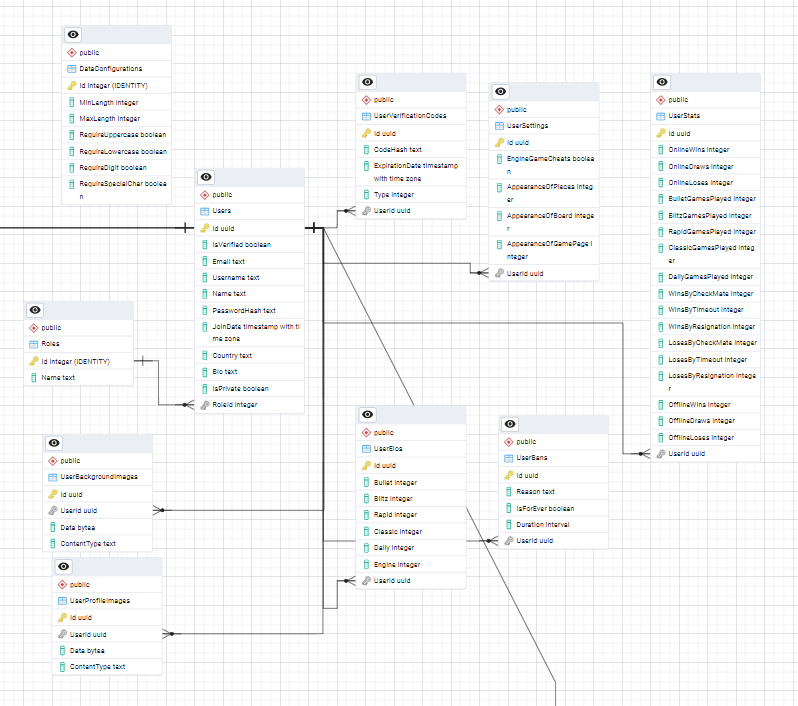
\includegraphics[width=0.8\textwidth]{zdj/user_ERD.png}
    \caption{Diagram relacji jednostka-relacja przedstawiający relacje użytkownika - wygenerowany za pomocą PgAdmin 4}
\end{figure}
\newpage

\noindent \textbf{Relacje znajomości} \\
Segment relacji przyjaźni jest zarządzany przez jednostkę przyjaźni, która reprezentuje połączenia społeczne między użytkownikami. Każda Encja Friendship ma dwóch kluczowych uczestników: Requestor (przyjmujacy) i Receiver (odbierający). Są to obaj użytkownicy, a relacje między tymi podmiotami są modelowane za pomocą kluczy obcych: RequestorId i ReceiverId. Ta relacja jest wiele-do-jednego, co oznacza, że użytkownik może mieć wiele przyjaźni zarówno jako żądający, jak i odbiorca. Dodatkowo, jednostka FriendshipStats śledzi statystyki związane z każdą przyjaźnią, tworząc relację jeden-do-jednego z jednostką Friendship.

\vspace{1cm}
\begin{figure}[h!]
    \centering
    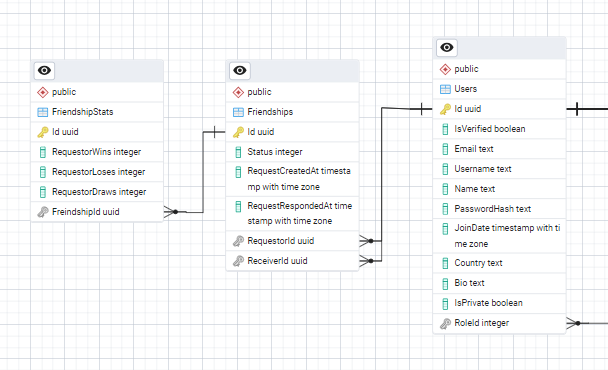
\includegraphics[width=0.8\textwidth]{zdj/friendship_ERD.png}
    \caption{Diagram relacji między podmiotami przedstawiający relacje przyjaźni między użytkownikami - wygenerowany za pomocą PgAdmin 4}
\end{figure}
\newpage

\noindent \textbf{Relacje w grach sieciowych} \\
Segment Web Game Relations obsługuje strukturę internetowej gry w szachy, z kilkoma jednostkami, które śledzą różne aspekty gry. Jednostka WebGame reprezentuje samą grę, łącząc graczy (WhitePlayer i BlackPlayer) poprzez relacje jeden-do-jednego. Stan i czas gry są kontrolowane przez encje WebGameState i WebGameTiming, które są połączone za pomocą kluczy obcych. Jednostka WebGamePlayer służy do śledzenia informacji specyficznych dla gracza dla każdej gry i odwołuje się do jednostki User. Ruchy wykonane w grze są przechowywane w encji WebGameMove, która ma relację wiele do jednego z WebGame. Dodatkowo, wiadomości wymieniane podczas gry są obsługiwane przez encje WebGameMessage i WebGamePlayerMessage, tworzące relacje odpowiednio z WebGame i WebGamePlayer.

\vspace{1cm}
\begin{figure}[h!]
    \centering
    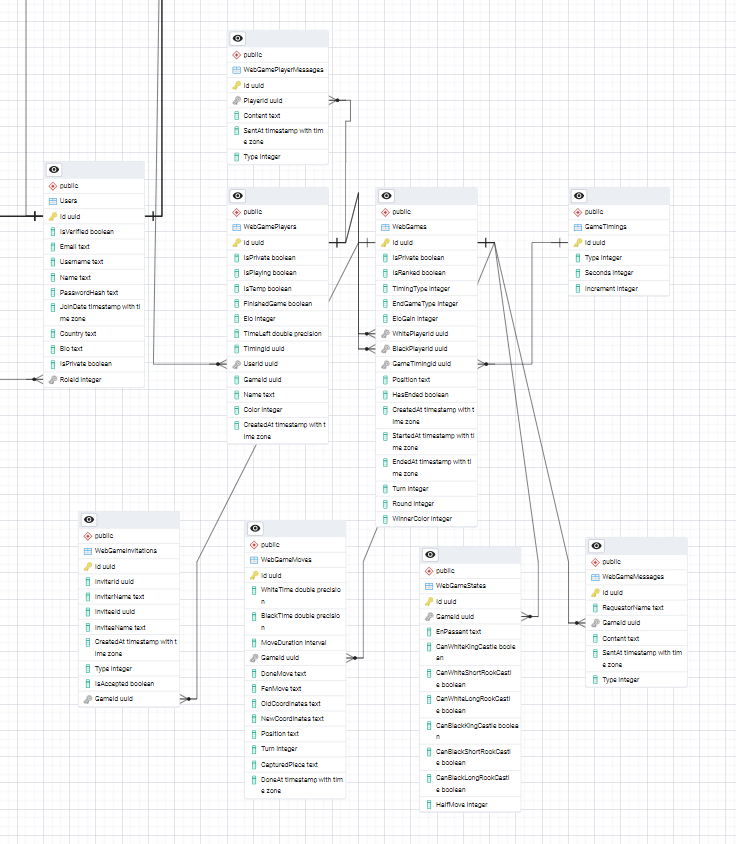
\includegraphics[width=0.8\textwidth]{zdj/online_ERD.png}
    \caption{Diagram relacji między podmiotami ilustrujący strukturę interakcji w grach sieciowych - wygenerowany za pomocą PgAdmin 4}
\end{figure}
\newpage

\noindent \textbf{Relacje w grach z silnikiem} \\
Segment ten skupia się na aspekcie gry opartym na silniku, gdzie każda gra jest zarządzana przez encję EngineGame. Encja EngineGame jest powiązana z encją EngineGamePlayer, reprezentującą użytkownika, który gra w grę opartą na silniku, a relacja jeden-do-jednego jest ustanawiana poprzez PlayerId. Każdy ruch w grze jest przechwytywany w encji EngineGameMove, która jest powiązana z encją EngineGame poprzez klucz obcy. Encja EngineGameState przechowuje aktualny stan gry opartej na silniku i jest powiązana z EngineGame poprzez relację jeden-do-jednego. Dodatkowo, wiadomości specyficzne dla gier silnikowych są przechowywane w encji EngineGameMessage, która jest powiązana z EngineGame poprzez klucz obcy.

\vspace{1cm}
\begin{figure}[h!]
    \centering
    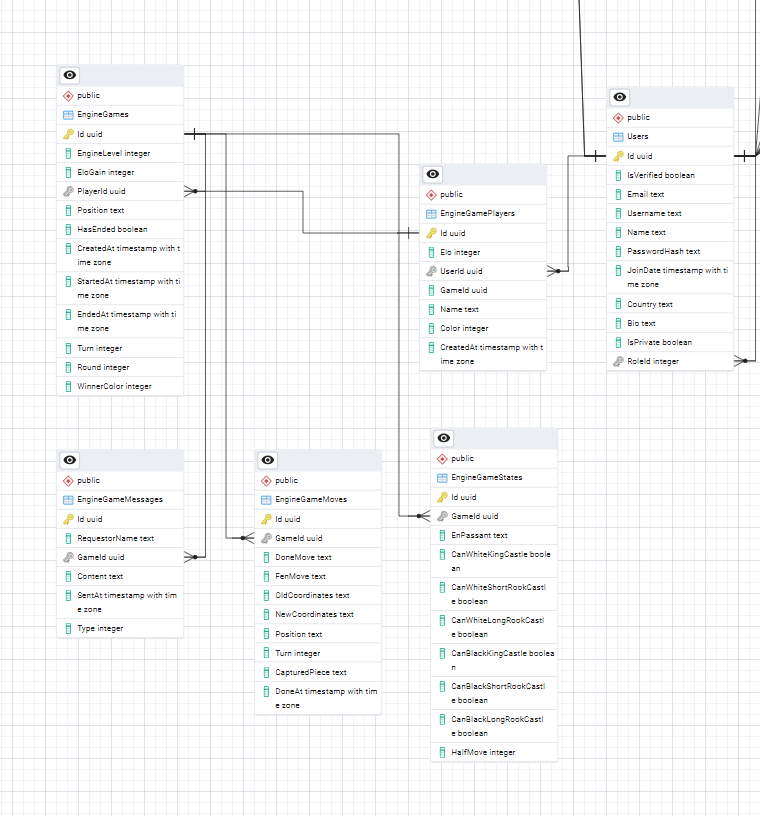
\includegraphics[width=0.8\textwidth]{zdj/offline_ERD.png}
    \caption{Diagram zależności między jednostkami przedstawiający relacje między silnikiem a grą - wygenerowany za pomocą PgAdmin 4}
\end{figure}
\newpage


\subsubsection{Opis encji}

\begin{itemize}
    \item \textbf{DataConfigurations} - Zawiera ustawienia konfiguracji dla kluczowych pól użytkownika.
    \begin{longtable}{|m{4cm}|m{2cm}|m{8cm}|}
        \hline
        \textbf{Właściwość} & \textbf{Typ} & \textbf{Opis} \\ \hline
        \endhead
        \hline
        Id & int & Identyfikator konfiguracji (PK) \\ \hline
        MinLength & int? & Minimalna długość pola \\ \hline
        MaxLength & int? & Maksymalna długość pola \\ \hline
        RequireUppercase & bool & Czy wymagana jest wielka litera \\ \hline
        RequireLowercase & bool & Czy wymagana jest mała litera \\ \hline
        RequireDigit & bool & Czy wymagana jest cyfra \\ \hline
        RequireSpecialChar & bool & Czy wymiany jest znak specjalny \\ \hline
    \end{longtable}

    \item \textbf{Roles} - Określa role użytkowników w systemie, takie jak "User" i "Admin".
    \begin{longtable}{|m{4cm}|m{2cm}|m{8cm}|}
        \hline
        \textbf{Właściwość} & \textbf{Typ} & \textbf{Opis} \\ \hline
        \endhead
        \hline
        Id & int & Identyfikator roli (PK) \\ \hline
        Name & string & Nazwa roli \\ \hline
    \end{longtable}

    \item \textbf{Users} - Główna encja reprezentująca użytkownika.
    \begin{longtable}{|m{4cm}|m{2cm}|m{8cm}|}
        \hline
        \textbf{Właściwość} & \textbf{Typ} & \textbf{Opis} \\ \hline
        \endhead
        \hline
        Id & Guid & Identyfikator użytkownika (PK) \\ \hline
        IsVerified & bool & Czy email użytkownika jest zweryfikowany \\ \hline
        Email & string & Adres email użytkownika \\ \hline
        Username & string & Unikalna nazwa użytkownika \\ \hline
        Name & string? & Pełne imię i nazwisko użytkownika \\ \hline
        PasswordHash & string & Zahashowane hasło użytkownika \\ \hline
        JoinDate & DateTime & Data dołączenia użytkownika do systemu \\ \hline
        Country & string & Kraj, w którym użytkownik się zarejestrował \\ \hline
        Bio & string? & Krótkie bio lub opis użytkownika \\ \hline
        IsPrivate & bool & Określa, czy profil użytkownika jest prywatny \\ \hline
        RoleId & int & Identyfikator roli użytkownika\\ \hline
    \end{longtable}

    \item \textbf{UserProfileImage} - zdjęcia profilowe użytkownika.
    \begin{longtable}{|m{4cm}|m{2cm}|m{8cm}|}
        \hline
        \textbf{Właściwość} & \textbf{Typ} & \textbf{Opis} \\ \hline
        \endhead
        \hline
        Id & Guid & Identyfikator obrazu użytkownika (PK) \\ \hline
        UserId & Guid & Identyfikator użytkownika do którego należy obraz \\ \hline
        Data & byte[] & Dane obrazu w postaci bajtów \\ \hline
        ContentType & string & Typ zawartości obrazu (np. "image/png", "image/jpeg") \\ \hline
    \end{longtable}
        
    \item \textbf{UserBackgroundImages} - tło profilu użytkownika.
    \begin{longtable}{|m{4cm}|m{2cm}|m{8cm}|}
        \hline
        \textbf{Właściwość} & \textbf{Typ} & \textbf{Opis} \\ \hline
        \endhead
        \hline
        Id & Guid & Identyfikator obrazu tła użytkownika (PK) \\ \hline
        UserId & Guid & Identyfikator użytkownika, do którego należy obraz tła \\ \hline
        Data & byte[] & Dane obrazu tła w postaci bajtów \\ \hline
        ContentType & string & Typ zawartości obrazu tła (np. "image/png", "image/jpeg") \\ \hline
    \end{longtable}
        
    \item \textbf{UserElos} - punktacja użytkownika dla poszczególnych trybów czasowych gry.
    \begin{longtable}{|m{4cm}|m{2cm}|m{8cm}|}
        \hline
        \textbf{Właściwość} & \textbf{Typ} & \textbf{Opis} \\ \hline
        \endhead
        \hline
        Id & Guid & Identyfikator ELO (PK) \\ \hline
        Bullet & int & Punkty ELO dla trybu Bullet \\ \hline
        Blitz & int & Punkty ELO dla trybu Blitz \\ \hline
        Rapid & int & Punkty ELO dla trybu Rapid \\ \hline
        Classic & int & Punkty ELO dla trybu Classic \\ \hline
        Daily & int & Punkty ELO dla trybu Daily \\ \hline
        Engine & int & Punkty ELO dla gier z silnikiem \\ \hline
        UserId & Guid & Identyfikator użytkownika, do którego należy ELO \\ \hline
    \end{longtable}
        
    \item \textbf{UserStats} - tablica statystyki użytkownika.
    \begin{longtable}{|m{4cm}|m{2cm}|m{8cm}|}
        \hline
        \textbf{Właściwość} & \textbf{Typ} & \textbf{Opis} \\ \hline
        \endhead
        \hline
        Id & Guid & Identyfikator statystyk użytkownika (PK) \\ \hline
        OnlineWins & int & Liczba wygranych gier online \\ \hline
        OnlineDraws & int & Liczba remisów gier online \\ \hline
        OnlineLoses & int & Liczba przegranych gier online \\ \hline
        OnlineGamesPlayed & int & Łączna liczba gier online \\ \hline
        BulletGamesPlayed & int & Liczba gier online w trybie Bullet \\ \hline
        BlitzGamesPlayed & int & Liczba gier online w trybie Blitz \\ \hline
        RapidGamesPlayed & int & Liczba gier online w trybie Rapid \\ \hline
        ClassicGamesPlayed & int & Liczba gier online w trybie Classic \\ \hline
        DailyGamesPlayed & int & Liczba gier online w trybie Daily \\ \hline
        WinsByCheckMate & int & Liczba wygranych przez mat \\ \hline
        WinsByTimeout & int & Liczba wygranych przez czas \\ \hline
        WinsByResignation & int & Liczba wygranych przez rezygnację \\ \hline
        LosesByCheckMate & int & Liczba przegranych przez mat \\ \hline
        LosesByTimeout & int & Liczba przegranych przez czas \\ \hline
        LosesByResignation & int & Liczba przegranych przez rezygnację \\ \hline
        OfflineWins & int & Liczba wygranych gier offline \\ \hline
        OfflineDraws & int & Liczba remisów gier offline \\ \hline
        OfflineLoses & int & Liczba przegranych gier offline \\ \hline
        OfflineGamesPlayed & int & Łączna liczba gier offline \\ \hline
        UserId & Guid & Identyfikator użytkownika, do którego należą statystyki \\ \hline
    \end{longtable}
        
    \item \textbf{UserSettings} - globalne ustawienia konta oraz gier.
    \begin{longtable}{|m{4cm}|m{2cm}|m{8cm}|}
        \hline
        \textbf{Właściwość} & \textbf{Typ} & \textbf{Opis} \\ \hline
        \endhead
        \hline
        Id & Guid & Identyfikator ustawień użytkownika (PK) \\ \hline
        EngineGameCheats & bool & Określa, czy oszustwa w grze silnikiem są dozwolone \\ \hline
        Ap-OfPieces & enum & Ustawienia wyglądu figur w grze \\ \hline
        Ap-OfBoard & enum & Ustawienia wyglądu planszy w grze \\ \hline
        Ap-OfGamePage & enum & Ustawienia wyglądu strony gry \\ \hline
        UserId & Guid & Identyfikator użytkownika, do którego należą ustawienia \\ \hline
    \end{longtable}

    \item \textbf{UserVerificationCodes} - tablica kodów weryfikacyjnych.
    \begin{longtable}{|m{4cm}|m{2cm}|m{8cm}|}
        \hline
        \textbf{Właściwość} & \textbf{Typ} & \textbf{Opis} \\ \hline
        \endhead
        \hline
        Id & Guid & Identyfikator kodu weryfikacyjnego (PK) \\ \hline
        CodeHash & string & Zahashowany kod używany do weryfikacji \\ \hline
        ExpirationDate & DateTime & Data wygaśnięcia kodu weryfikacyjnego \\ \hline
        Type & enum & Typ kodu weryfikacyjnego \\ \hline
        UserId & Guid & Identyfikator użytkownika, do którego należy kod weryfikacyjny \\ \hline
    \end{longtable}

    \item \textbf{Friendships} - tablica relacji pomiędzy użytkownikami.
    \begin{longtable}{|m{4cm}|m{2cm}|m{8cm}|}
        \hline
        \textbf{Właściwość} & \textbf{Typ} & \textbf{Opis} \\ \hline
        \endhead
        \hline
        Id & Guid & Identyfikator relacji przyjaźni (PK) \\ \hline
        Status & enum & Status przyjaźni  \\ \hline
        RequestCreatedAt & DateTime & Data utworzenia/złożenia wniosku o przyjaźń \\ \hline
        RequestRespondedAt & DateTime? & Data, kiedy druga strona odpowiedziała na wniosek o przyjaźń \\ \hline
        RequestorId & Guid & Identyfikator użytkownika, który wysłał prośbę o przyjaźń \\ \hline
        ReceiverId & Guid & Identyfikator użytkownika, który otrzymał prośbę o przyjaźń \\ \hline
    \end{longtable}
        
  
    \item \textbf{FriendshipStats} - Statystki dotyczące relacji uzytkownikow.
    \begin{longtable}{|m{4cm}|m{2cm}|m{8cm}|}
        \hline
        \textbf{Właściwość} & \textbf{Typ} & \textbf{Opis} \\ \hline
        \endhead
        \hline
        Id & Guid & Identyfikator statystyk przyjaźni (PK) \\ \hline
        RequestorWins & int & Liczba wygranych przez osobę, która wysłała prośbę o przyjaźń \\ \hline
        RequestorLoses & int & Liczba przegranych przez osobę, która wysłała prośbę o przyjaźń \\ \hline
        RequestorDraws & int & Liczba remisów osoby, która wysłała prośbę o przyjaźń \\ \hline
        GamesPlayed & int & Łączna liczba rozegranych gier w relacji \\ \hline
        FriendshipId & Guid & Identyfikator relacji przyjaźni, do której należą statystyki \\ \hline
    \end{longtable}
        
    \item \textbf{WebGames} - Gry online między użytkownikami.
    \begin{longtable}{|m{4cm}|m{2cm}|m{8cm}|}
        \hline
        \textbf{Właściwość} & \textbf{Typ} & \textbf{Opis} \\ \hline
        \endhead
        \hline
        Id & Guid & Identyfikator gry online (PK) \\ \hline
        IsPrivate & bool & Określa, czy gra jest prywatna czy publiczna \\ \hline
        IsRanked & bool & Określa, czy gra będzie miała wpływ na ranking Elo \\ \hline
        TimingType & enum & Typ czasu gry (np. Bullet, Blitz, Rapid) \\ \hline
        EndGameType & enum? & Powód zakończenia gry (np. mat, czas) \\ \hline
        EloGain & int & Zysk lub strata Elo po zakończeniu gry \\ \hline
        WhitePlayerId & Guid & Identyfikator gracza grającego białymi \\ \hline
        BlackPlayerId & Guid & Identyfikator gracza grającego czarnymi \\ \hline
        GameTimingId & Guid & Identyfikator ustawień czasu gry \\ \hline
        Position & string & Aktualna pozycja na szachownicy \\ \hline
        HasEnded & bool & Flaga, czy gra się zakończyła \\ \hline
        CreatedAt & DateTime & Data utworzenia gry \\ \hline
        StartedAt & DateTime? & Data rozpoczęcia gry \\ \hline
        EndedAt & DateTime? & Data zakończenia gry \\ \hline
        Turn & int & Numer tury gry \\ \hline
        Round & int & Numer rundy \\ \hline
        WinnerColor & enum? & Kolor zwycięzcy (null oznacza remis) \\ \hline
    \end{longtable}
        
        
 
    \item \textbf{GameTimings} - kontrole czasowe dla gier z ograniczeniem czasu.
    \begin{longtable}{|m{4cm}|m{2cm}|m{8cm}|}
        \hline
        \textbf{Właściwość} & \textbf{Typ} & \textbf{Opis} \\ \hline
        \endhead
        \hline
        Id & Guid & Identyfikator ustawienia czasu gry (PK) \\ \hline
        Type & enum & Typ czasu (np. Bullet, Rapid) \\ \hline
        Seconds & int & Czas trwania gry w sekundach \\ \hline
        Increment & int & Inkrement czasowy w sekundach \\ \hline
    \end{longtable}
        

    \item \textbf{WebGameStates} - Stan gry online, przechowuje dane szczególne dotyczące obecnej gry.
    \begin{longtable}{|m{4cm}|m{2cm}|m{8cm}|}
        \hline
        \textbf{Właściwość} & \textbf{Typ} & \textbf{Opis} \\ \hline
        \endhead
        \hline
        Id & Guid & Identyfikator stanu gry (PK) \\ \hline
        GameId & Guid & Identyfikator gry, do której należy stan \\ \hline
        EnPassant & string? & Koordynaty dla ruchu en passant w formacie x,y \\ \hline
        CWKing & bool & Czy biały król może jeszcze wykonać roszadę \\ \hline
        CWShort & bool & Czy biały król może wykonać krótką roszadę \\ \hline
        CWLong & bool & Czy biały król może wykonać długą roszadę \\ \hline
        CBKing & bool & Czy czarny król może jeszcze wykonać roszadę \\ \hline
        CBShort & bool & Czy czarny król może wykonać krótką roszadę \\ \hline
        CBLong & bool & Czy czarny król może wykonać długą roszadę \\ \hline
        HalfMove & int & Liczba ruchów nie będących ruchem pionkiem (dla zasady 50 ruchów) \\ \hline
    \end{longtable}
        

    \item \textbf{WebGameInvitations} - Opcjonalne zaproszenia do gry.
    \begin{longtable}{|m{4cm}|m{2cm}|m{8cm}|}
        \hline
        \textbf{Właściwość} & \textbf{Typ} & \textbf{Opis} \\ \hline
        \endhead
        \hline
        Id & Guid & Identyfikator zaproszenia (PK) \\ \hline
        InviterId & Guid & Identyfikator użytkownika zapraszającego \\ \hline
        InviterName & string & Nazwa użytkownika zapraszającego \\ \hline
        InviteeId & Guid & Identyfikator użytkownika zapraszanego \\ \hline
        InviteeName & string & Nazwa użytkownika zapraszanego \\ \hline
        CreatedAt & DateTime & Data utworzenia zaproszenia \\ \hline
        Type & enum & Typ czasu gry, do którego odnosi się zaproszenie \\ \hline
        IsAccepted & bool & Flaga, która wskazuje, czy zaproszenie zostało zaakceptowane \\ \hline
        GameId & Guid & Identyfikator gry, do której zaproszenie należy \\ \hline
    \end{longtable}
        

    \item \textbf{WebGameMessages} - Wiadomości systemowe dotyczące gry online.
    \begin{longtable}{|m{4cm}|m{2cm}|m{8cm}|}
        \hline
        \textbf{Właściwość} & \textbf{Typ} & \textbf{Opis} \\ \hline
        \endhead
        \hline
        Id & Guid & Identyfikator wiadomości (PK) \\ \hline
        RequestorName & string & Nazwa użytkownika, który zażądał remisu \\ \hline
        GameId & Guid & Identyfikator gry, do której wiadomość należy \\ \hline
        Content & string & Treść wiadomości \\ \hline
        SentAt & DateTime & Data i godzina wysłania wiadomości \\ \hline
        Type & enum & Typ wiadomości (np. prośba o remis) \\ \hline
    \end{longtable}
        

    \item \textbf{WebGameMove} - Ruchy wykonane podczas gry online.
    \begin{longtable}{|m{4cm}|m{2cm}|m{8cm}|}
        \hline
        \textbf{Właściwość} & \textbf{Typ} & \textbf{Opis} \\ \hline
        \endhead
        \hline
        Id & Guid & Identyfikator ruchu (PK) \\ \hline
        WhiteTime & double & Czas pozostały dla białego gracza \\ \hline
        BlackTime & double & Czas pozostały dla czarnego gracza \\ \hline
        MoveDuration & TimeSpan & Czas, który gracz zużył na wykonanie ruchu \\ \hline
        GameId & Guid & Identyfikator gry, do której ruch należy \\ \hline
        DoneMove & string & Wykonany ruch w formacie: tag figury + x (jeśli zbicie) + współrzędne xy \\ \hline
        FenMove & string & Wykonany ruch w formacie FEN \\ \hline
        OldCoordinates & string & Współrzędne, z których figura została przemieszczona w formacie x,y \\ \hline
        NewCoordinates & string & Współrzędne, na które figura została przemieszczona w formacie x,y \\ \hline
        Position & string & Pozycja na szachownicy po wykonaniu ruchu \\ \hline
        Turn & int & Tura, w której ruch został wykonany \\ \hline
        CapturedPiece & string? & Tag zbitej figury \\ \hline
        DoneAt & DateTime & Data i godzina wykonania ruchu \\ \hline
    \end{longtable}
        
    \item \textbf{WebGamePlayers} - Tablica graczy gry online.
    \begin{longtable}{|m{4cm}|m{2cm}|m{8cm}|}
        \hline
        \textbf{Właściwość} & \textbf{Typ} & \textbf{Opis} \\ \hline
        \endhead
        \hline
        Id & Guid & Identyfikator gracza (PK) \\ \hline
        IsPrivate & bool & Określa, czy gracz może być używany w globalnym wyszukiwaniu, czy jest tylko dla prywatnej gry \\ \hline
        IsPlaying & bool & Flaga, czy gracz wciąż szuka gry \\ \hline
        IsTemp & bool & Flaga, czy gracz jest tymczasowy \\ \hline
        FinishedGame & bool & Flaga, czy gra dla gracza została zakończona \\ \hline
        Elo & int & Punkty Elo dla konkretnego typu czasu \\ \hline
        TimeLeft & double & Czas pozostały na wykonanie ruchów zgodnie z czasem gry \\ \hline
        TimingId & Guid & Identyfikator typu czasu, określający czas trwania i przyrost czasu dla wszystkich ruchów \\ \hline
        UserId & Guid & Identyfikator użytkownika, któremu gracz należy \\ \hline
        GameId & Guid & Identyfikator gry, w której gracz bierze udział \\ \hline
        Name & string & Nazwa gracza (nazwa użytkownika) \\ \hline
        Color & enum? & Kolor gracza (czarny lub biały), null jeśli gracz szuka jeszcze gry \\ \hline
        CreatedAt & DateTime & Data utworzenia gracza \\ \hline
    \end{longtable}

    \item \textbf{WebGamePlayerMessages} - wiadomości wysłane przez graczy podczas gry online.
    \begin{longtable}{|m{4cm}|m{2cm}|m{8cm}|}
        \hline
        \textbf{Właściwość} & \textbf{Typ} & \textbf{Opis} \\ \hline
        \endhead
        \hline
        Id & Guid & Identyfikator wiadomości (PK) \\ \hline
        PlayerId & Guid & Identyfikator gracza, który wysłał wiadomość \\ \hline
        Content & string & Treść wiadomości \\ \hline
        SentAt & DateTime & Data i czas wysłania wiadomości \\ \hline
        Type & enum & Typ wiadomości \\ \hline
    \end{longtable}
        
    \item \textbf{EngineGames} - Tablica gier offline z silnikiem szachowym. 
    \begin{longtable}{|m{4cm}|m{2cm}|m{8cm}|}
        \hline
        \textbf{Właściwość} & \textbf{Typ} & \textbf{Opis} \\ \hline
        \endhead
        \hline
        Id & Guid & Identyfikator gry (PK) \\ \hline
        EngineLevel & int & Poziom głębokości silnika \\ \hline
        EloGain & int & Zysk lub strata Elo po zakończeniu gry \\ \hline
        PlayerId & Guid & Identyfikator gracza \\ \hline
        Position & string & Aktualna pozycja w grze \\ \hline
        HasEnded & bool & Flaga informująca, czy gra zakończona \\ \hline
        CreatedAt & DateTime & Data utworzenia gry \\ \hline
        StartedAt & DateTime? & Data rozpoczęcia gry \\ \hline
        EndedAt & DateTime? & Data zakończenia gry \\ \hline
        Turn & int & Numer tury gry \\ \hline
        Round & int & Numer rundy gry (pełny ruch) \\ \hline
        WinnerColor & enum? & Kolor zwycięzcy (null oznacza remis) \\ \hline
    \end{longtable}

    
    \item \textbf{EngineGameStates} - Stan gry offline, przechowuje dane szczególne dotyczące obecnej gry.
    \begin{longtable}{|m{4cm}|m{2cm}|m{8cm}|}
        \hline
        \textbf{Właściwość} & \textbf{Typ} & \textbf{Opis} \\ \hline
        \endhead
        \hline
        Id & Guid & Identyfikator stanu gry (PK) \\ \hline
        GameId & Guid & Identyfikator gry, do której należy stan \\ \hline
        EnPassant & string? & Współrzędne en passant, jeśli możliwe, w formacie x,y \\ \hline
        CWKing & bool & Czy biały król może jeszcze wykonać roszadę \\ \hline
        CWShort & bool & Czy biały król może wykonać krótką roszadę \\ \hline
        CWLong & bool & Czy biały król może wykonać długą roszadę \\ \hline
        CBKing & bool & Czy czarny król może jeszcze wykonać roszadę \\ \hline
        CBShort & bool & Czy czarny król może wykonać krótką roszadę \\ \hline
        CBLong & bool & Czy czarny król może wykonać długą roszadę \\ \hline
        HalfMove & int & Liczba ruchów wykonanych przez graczy, z wyjątkiem pionków, dla zasady 50 ruchów \\ \hline
    \end{longtable}
    

    \item \textbf{EngineGamePlayers} - Gracze gier offline.
    \begin{longtable}{|m{4cm}|m{2cm}|m{8cm}|}
        \hline
        \textbf{Właściwość} & \textbf{Typ} & \textbf{Opis} \\ \hline
        \endhead
        \hline
        Id & Guid & Identyfikator gracza (PK) \\ \hline
        Elo & int & Punkty Elo dla gier przeciwko silnikowi \\ \hline
        UserId & Guid & Identyfikator użytkownika, do którego należy gracz \\ \hline
        GameId & Guid & Identyfikator gry, w której gracz bierze udział \\ \hline
        Name & string & Nazwa użytkownika (imię gracza) \\ \hline
        Color & enum? & Kolor gracza (czarny lub biały), null oznacza oczekiwanie na grę \\ \hline
        CreatedAt & DateTime & Data utworzenia gracza (do kolejek oczekujących) \\ \hline
    \end{longtable}
    
    \item \textbf{EngineGameMoves} - Ruchy wykonane podczas gry offline.
    \begin{longtable}{|m{4cm}|m{2cm}|m{8cm}|}
        \hline
        \textbf{Właściwość} & \textbf{Typ} & \textbf{Opis} \\ \hline
        \endhead
        \hline
        Id & Guid & Identyfikator ruchu (PK) \\ \hline
        GameId & Guid & Identyfikator gry, do której należy ruch \\ \hline
        DoneMove & string & Wykonany ruch w formacie: oznaczenie figury + x (jeśli zbicie) + współrzędne xy \\ \hline
        FenMove & string & Wykonany ruch w formacie FEN \\ \hline
        OldCoordinates & string & Współrzędne, z których figura została przesunięta (format "x,y") \\ \hline
        NewCoordinates & string & Współrzędne, na które figura została przesunięta (format "x,y") \\ \hline
        Position & string & Pozycja po wykonaniu ruchu \\ \hline
        Turn & int & Tura, w której wykonano ruch \\ \hline
        CapturedPiece & string? & Zbita figura, jeśli dotyczy \\ \hline
        DoneAt & DateTime & Data i godzina wykonania ruchu \\ \hline
    \end{longtable}
    
    \item \textbf{EngineGameMessages} - Automatyczne wiadomości dotyczące gry offline.
    \begin{longtable}{|m{4cm}|m{2cm}|m{8cm}|}
        \hline
        \textbf{Właściwość} & \textbf{Typ} & \textbf{Opis} \\ \hline
        \endhead
        \hline
        Id & Guid & Identyfikator wiadomości (PK) \\ \hline
        RequestorName & string & Nazwa osoby lub systemu wysyłającego wiadomość (domyślnie "BRN CHess") \\ \hline
        GameId & Guid & Identyfikator gry, do której należy wiadomość \\ \hline
        Content & string & Treść wiadomości \\ \hline
        SentAt & DateTime & Data i godzina wysłania wiadomości \\ \hline
        Type & enum & Typ wiadomości \\ \hline
    \end{longtable}
    
\end{itemize}

\newpage

\subsection{Backend}
\subsubsection{Architektura}

\begin{figure}[h!]
    \centering
    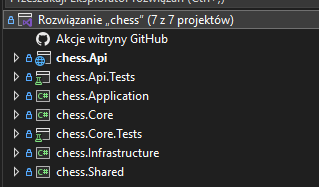
\includegraphics[width=0.6\textwidth]{zdj/struktura_back.png}
    \caption{Struktura.}
\end{figure}

\newpage

\begin{minipage}[t]{0.45\textwidth}
    \vspace{0pt}
    \raggedright
    \lipsum[1] 
\end{minipage}
\hfill
\begin{minipage}[t]{0.45\textwidth}
    \vspace{0pt}
    \centering
    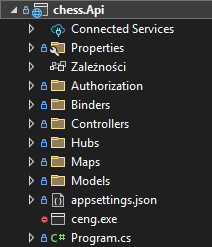
\includegraphics[width=\linewidth]{zdj/struktura_back_api.png}
\end{minipage}

\vspace{1cm}

\begin{minipage}[t]{0.45\textwidth}
    \vspace{0pt}
    \centering
    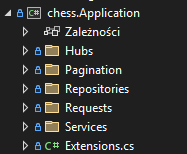
\includegraphics[width=\linewidth]{zdj/struktura_back_application.png} 
\end{minipage}
\hfill
\begin{minipage}[t]{0.45\textwidth}
    \vspace{0pt}
    \raggedright
    \lipsum[2] 
\end{minipage}

\vspace{1cm}

\begin{minipage}[t]{0.45\textwidth}
    \vspace{0pt}
    \raggedright
    \lipsum[3] 
\end{minipage}
\hfill
\begin{minipage}[t]{0.45\textwidth}
    \vspace{0pt}
    \centering
    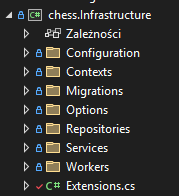
\includegraphics[width=\linewidth]{zdj/struktura_back_infrastructure.png} 
\end{minipage}

\vspace{1cm}

\begin{minipage}[t]{0.45\textwidth}
    \vspace{0pt}
    \centering
    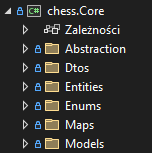
\includegraphics[width=\linewidth]{zdj/struktura_back_core.png} 
\end{minipage}
\hfill
\begin{minipage}[t]{0.45\textwidth}
    \vspace{0pt}
    \raggedright
    \lipsum[4] 
\end{minipage}

\vspace{1cm}

\begin{minipage}[t]{0.45\textwidth}
    \vspace{0pt}
    \raggedright
    \lipsum[5] 
\end{minipage}
\hfill
\begin{minipage}[t]{0.45\textwidth}
    \vspace{0pt}
    \centering
    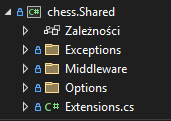
\includegraphics[width=\linewidth]{zdj/struktura_back_shared.png} 
\end{minipage}

\vspace{1cm}

\begin{minipage}[t]{0.45\textwidth}
    \vspace{0pt}
    \centering
    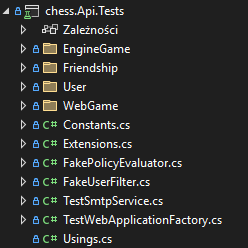
\includegraphics[width=\linewidth]{zdj/struktura_back_api_tests.png} 
\end{minipage}
\hfill
\begin{minipage}[t]{0.45\textwidth}
    \vspace{0pt}
    \raggedright
    \lipsum[6] 
\end{minipage}

\vspace{1cm}

\begin{minipage}[t]{0.45\textwidth}
    \vspace{0pt}
    \raggedright
    \lipsum[7] 
\end{minipage}
\hfill
\begin{minipage}[t]{0.45\textwidth}
    \vspace{0pt}
    \centering
    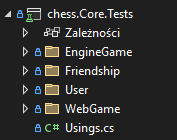
\includegraphics[width=\linewidth]{zdj/struktura_back_core_tests.png} 
\end{minipage}

\newpage

\begin{figure}[h!]
    \centering
    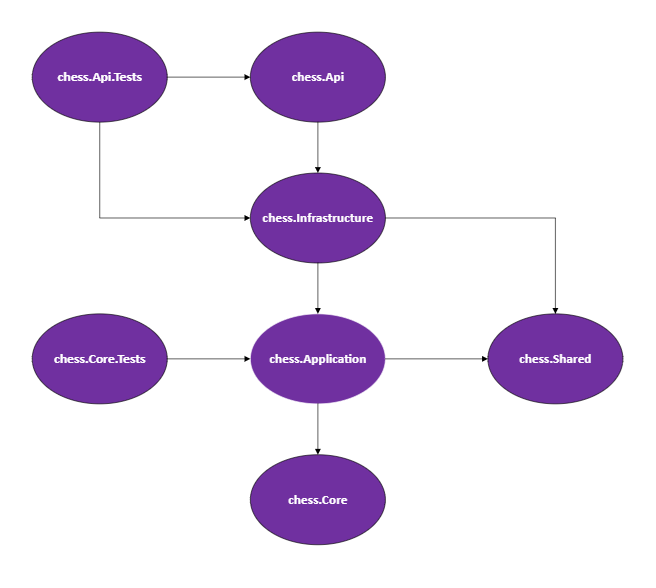
\includegraphics[width=1\textwidth]{zdj/backend_dependencies.png}
    \caption{Zależności.}
\end{figure}

\newpage

\subsubsection{Wykorzystane pakiety i biblioteki}

W projekcie zastosowano szereg bibliotek, które wspierają rozwój i funkcjonalność aplikacji. Każda z wymienionych bibliotek została dobrana w celu spełnienia konkretnych wymagań funkcjonalnych i architektonicznych projektu, co pozwala na jego rozwój zgodny z najlepszymi praktykami. Poniżej przedstawiono szczegółowy opis wybranych komponentów:
\begin{itemize}
    \item \textbf{SignalRSwaggerGen}: SignalRSwaggerGen umożliwia integrację SignalR z generatorem dokumentacji Swagger. Dzięki temu można dokumentować huby SignalR w podobny sposób, jak w przypadku typowych API REST. To znacznie upraszcza korzystanie z SignalR w projektach, gdzie przejrzystość i zrozumiałość API jest kluczowa.
    \item \textbf{Swashbuckle.AspNetCore}: Swashbuckle to jedno z najpopularniejszych narzędzi do generowania dokumentacji Swagger w projektach ASP.NET Core. Umożliwia automatyczne generowanie interaktywnej dokumentacji API, która może być używana do testowania endpointów bezpośrednio z poziomu przeglądarki.
    \item \textbf{AutoMapper}: AutoMapper jest biblioteką ułatwiającą mapowanie obiektów, co pozwala na szybkie i bezbłędne przekształcanie danych pomiędzy różnymi warstwami aplikacji, np. z warstwy domenowej na DTO (Data Transfer Object) i odwrotnie. Dzięki temu eliminuje potrzebę ręcznego mapowania, co zmniejsza ryzyko błędów i przyspiesza rozwój.
    \item \textbf{MediatR}: MediatR implementuje wzorzec Mediatora, umożliwiając luźne powiązania pomiędzy komponentami aplikacji. Jest szeroko stosowany w aplikacjach opartych na wzorcu CQRS (Command Query Responsibility Segregation). Dzięki MediatR można łatwo zarządzać logiką obsługi zdarzeń i zapytań, co poprawia modularność i testowalność kodu.
    \item \textbf{Npgsql.EntityFrameworkCore.PostgreSQL}: Jest to dostawca Entity Framework Core dla bazy danych PostgreSQL. Umożliwia korzystanie z zaawansowanych funkcji PostgreSQL, takich jak typy JSON, tablice czy rozszerzenia specyficzne dla tej bazy danych, bezpośrednio w ramach Entity Framework Core.
    \item \textbf{FluentAssertions}: FluentAssertions to biblioteka, która rozszerza możliwości standardowych asercji w testach jednostkowych. Umożliwia pisanie bardziej czytelnych i wyrażających zamiar asercji, takich jak result.Should().Be(expected) zamiast standardowego Assert.AreEqual(expected, result). Jest szeroko wykorzystywana w testach jednostkowych, ponieważ zapewnia lepszą czytelność i kontrolę nad wynikami testów.

    \item \textbf{Microsoft.AspNetCore.SignalR}: To biblioteka w ekosystemie .NET, która umożliwia łatwe dodanie funkcjonalności komunikacji w czasie rzeczywistym do aplikacji webowych. SignalR abstrahuje nad złożonością protokołów komunikacji (takich jak WebSockets, Long Polling) i pozwala na łatwą wymianę danych w czasie rzeczywistym między serwerem a klientami, bez konieczności odświeżania strony. SignalR jest szczególnie użyteczny w aplikacjach wymagających bieżącej interakcji z użytkownikiem, takich jak czaty, powiadomienia, gry online, a także aplikacje, które wymagają synchronizacji danych w czasie rzeczywistym (np. aplikacje finansowe, analityczne).
    \item \textbf{Microsoft.AspNetCore.OpenApi}: Biblioteka ta umożliwia integrację z OpenAPI, co pozwala na automatyczne generowanie dokumentacji API. Jest to szczególnie użyteczne w przypadku projektów opartych na architekturze REST, ponieważ pozwala deweloperom i użytkownikom końcowym lepiej rozumieć działanie aplikacji oraz dostępne endpointy.
    \item \textbf{Microsoft.AspNetCore.Cors}: Biblioteka ta obsługuje Cross-Origin Resource Sharing (CORS), co umożliwia kontrolowanie, które domeny mają dostęp do zasobów serwera. Jest to kluczowe w aplikacjach internetowych komunikujących się z frontendem hostowanym na innych domenach.
    \item \textbf{Microsoft.AspNetCore.Identity}: Microsoft.AspNetCore.Identity dostarcza rozbudowany framework do zarządzania użytkownikami, rolami, uwierzytelnianiem i autoryzacją. Umożliwia łatwą integrację takich funkcji, jak rejestracja, logowanie, resetowanie haseł czy zarządzanie rolami użytkowników.
    \item \textbf{Microsoft.AspNetCore.Http.Abstractions}: Biblioteka dostarcza podstawowe interfejsy i klasy wspierające obsługę żądań i odpowiedzi HTTP w aplikacjach ASP.NET Core. Umożliwia budowanie lekkich middleware oraz operacje na poziomie HTTP, takie jak praca z HttpContext.
    \item \textbf{Microsoft.AspNetCore.Authentication.JwtBearer}: Biblioteka ta obsługuje uwierzytelnianie oparte na JWT (JSON Web Tokens) w aplikacjach ASP.NET Core. Jest często używana w nowoczesnych aplikacjach webowych i API do implementacji bezpiecznych mechanizmów uwierzytelniania i autoryzacji.
    \item \textbf{Microsoft.AspNetCore.Mvc.Core}: Biblioteka ta zawiera podstawowe funkcje MVC (Model-View-Controller) dla aplikacji ASP.NET Core. Jest wykorzystywana do budowy endpointów API oraz obsługi żądań HTTP, zapewniając spójność i elastyczność w projektowaniu warstwy prezentacji i komunikacji.
    \item \textbf{Microsoft.AspNetCore.Mvc.Testing}: Biblioteka ta umożliwia łatwe testowanie aplikacji ASP.NET Core z wykorzystaniem WebApplicationFactory, które pozwala na uruchomienie aplikacji w testowym środowisku. Jest to kluczowa biblioteka do testów integracyjnych, ponieważ pozwala na testowanie całej aplikacji lub jej części, w tym kontrolerów, routingu i middleware, bez potrzeby uruchamiania pełnego serwera.
    \item \textbf{Microsoft.IdentityModel.Tokens}: Jest to kluczowa biblioteka do obsługi tokenów, takich jak JWT (JSON Web Tokens). Umożliwia tworzenie i weryfikację tokenów, co jest niezbędne w aplikacjach z uwierzytelnianiem i autoryzacją opartą na tokenach.
    \item \textbf{Microsoft.EntityFrameworkCore}: Entity Framework Core to nowoczesny ORM (Object-Relational Mapper) dla platformy .NET. Umożliwia łatwe mapowanie obiektów w aplikacji na tabele w relacyjnej bazie danych. Zapewnia wsparcie dla wielu funkcji, takich jak zapytania LINQ, migracje schematów bazy danych czy śledzenie zmian w danych.
    \item \textbf{Microsoft.EntityFrameworkCore.Tools}: Narzędzie wspomagające pracę z Entity Framework Core. Umożliwia m.in. zarządzanie migracjami, tworzenie baz danych na podstawie modelu aplikacji oraz generowanie kodu odwrotnego (reverse engineering) z istniejącej bazy danych. Ustawienie PrivateAssets na all powoduje, że biblioteka ta nie jest uwzględniana w pakiecie wynikowym, ponieważ jej funkcje są wykorzystywane głównie podczas rozwoju aplikacji.
    \item \textbf{Microsoft.EntityFrameworkCore.Design}: Ta biblioteka jest rozszerzeniem Entity Framework Core, które wspiera projektowanie i migrację baz danych. Dzięki niej można korzystać z narzędzi takich jak dotnet ef, które umożliwiają m.in. generowanie schematów baz danych, zarządzanie migracjami i synchronizowanie modeli danych z bazą.
    \item \textbf{Microsoft.EntityFrameworkCore.InMemory}: Biblioteka ta jest implementacją bazy danych w pamięci (in-memory) dla Entity Framework Core. Umożliwia testowanie kodu, który współpracuje z bazą danych, bez potrzeby jej fizycznego uruchamiania. Jest to przydatne do testów jednostkowych i integracyjnych, gdzie potrzebne jest środowisko bazy danych, ale bez potrzeby używania rzeczywistego silnika bazy danych.
    \item \textbf{Microsoft.Extensions.DependencyInjection}: Biblioteka ta dostarcza mechanizm wstrzykiwania zależności (Dependency Injection), co jest kluczowym elementem w projektowaniu nowoczesnych aplikacji. Dzięki niej można łatwo zarządzać cyklem życia obiektów, zmniejszając ich wzajemne powiązania.
    \item \textbf{Microsoft.Extensions.DependencyInjection.Abstractions}: Dostarcza interfejsy oraz bazowe klasy do wstrzykiwania zależności (Dependency Injection). Pozwala na definiowanie i zarządzanie cyklem życia usług w aplikacji oraz wspiera luźne powiązanie komponentów, co jest kluczowe dla skalowalności i łatwości testowania kodu.
    \item \textbf{Microsoft.Extensions.Configuration.Abstractions}: Biblioteka ta zapewnia interfejsy i podstawowe klasy do obsługi konfiguracji aplikacji. Umożliwia zarządzanie ustawieniami aplikacji z różnych źródeł, takich jak pliki JSON, zmienne środowiskowe czy dostawcy niestandardowi.
    \item \textbf{Microsoft.Extensions.Configuration.Binder}: Biblioteka rozszerza możliwości systemu konfiguracji o mechanizm mapowania ustawień na typy obiektowe. Pozwala na łatwe wiązanie konfiguracji (np. z plików JSON) z obiektami w kodzie, dzięki czemu zarządzanie ustawieniami staje się bardziej przejrzyste i zorganizowane.

    \item \textbf{Microsoft.NET.Test.Sdk}: Jest to biblioteka wspierająca framework testowy w ekosystemie .NET. Zawiera narzędzia do uruchamiania testów, generowania raportów oraz integracji z narzędziami do testowania. Jest to podstawowy komponent, który umożliwia działanie testów w projektach .NET.
    \item \textbf{xUnit}: xUnit to jeden z popularniejszych frameworków testowych w ekosystemie .NET. Wspiera różne typy testów, takie jak testy jednostkowe, integracyjne, a także dostarcza zaawansowane funkcje, takie jak asercje, zestawy danych do testów czy zarządzanie cyklem życia testów.
    \item \textbf{xUnit.runner.visualstudio}: Biblioteka ta integruje xUnit z Visual Studio, umożliwiając uruchamianie testów i przeglądanie wyników testów bezpośrednio w interfejsie użytkownika Visual Studio. Dzięki temu programiści mogą wygodnie wykonywać testy i analizować ich wyniki.
    \item \textbf{Moq}: Moq to biblioteka do tworzenia obiektów "mock" (symulujących) w testach jednostkowych. Umożliwia zastąpienie prawdziwych zależności fałszywymi obiektami, co pozwala na testowanie logiki aplikacji w izolacji i bez potrzeby uruchamiania rzeczywistych komponentów zewnętrznych, takich jak bazy danych czy serwisy.
\end{itemize}

\newpage
\subsubsection{REST API}

Interfejsy API są najpopularniejszym sposobem interakcji programów i urządzeń w nowoczesnych technologiach obliczeniowych. API to zestaw reguł opisujących, jak jeden program może się łączyć oraz komunikować z innym. Jak sama nazwa wskazuje, API REST przekazuje na każde żądanie stan każdej transakcji, co daje korzyści związane z opracowaniem, wydajnością i zasobami w porównaniu do innych metod. REST rozwija się w ciągu ponad dwóch dekad i jest bardzo powszechnym podejściem do architektur opartych na usługach i architektur rozproszonych.
\\\\
Zasób jest podstawowym pojęciem dla API REST. Zasób jest obiektem, który ma typ, powiązane dane, relacje z innymi zasobami i zestaw metod, które na nim działają. Jest bardzo podobny do idei obiektów w programowaniu, chociaż zdefiniowanych jest tylko kilka standardowych metod, typowych dla HTTP GET, POST, PUT i DELETE. Zasoby mogą istnieć same lub w zbiorach, które same są zasobami.
\\\\
W nowoczesnej informatyce wspólnym modelem - również podstawowym dla API REST - jest klient-serwer, gdzie klient, który potrzebuje zasobu, identyfikuje się i komunikuje z serwerem, który może go dostarczyć. W ten sposób zarządzany jest praktycznie cały ruch w chmurze, gdyż oferuje maksymalną elastyczność licznym klientom i pozwala na dostęp do licznych serwerów. Zasada ta sprawdza się również w przypadku tzw. architektur „bezserwerowych", w których miejsce serwera znanego klientowi zajmuje broker usług.

\begin{minted}[fontsize=\small, bgcolor=lightgray]{csharp}
    [HttpPost("start")]
    [Authorize(Policy = "IsVerified")]
    public async Task<IActionResult> StartEngineGame([FromBody] StartEngineGameModel model) {
    
        var request = _mapper.Map<StartEngineGameRequest>(model);
    
        var result = await _mediator.Send(request);
    
        return Ok(result);
    }
\end{minted}

\newpage

\textbf{Endpointy}
\begin{itemize}
    \item \textbf{UserController}
    \begin{itemize} 
        \item \textbf{POST /api/user/sign-up} - Rejestruje użytkownika i wysyła kod weryfikacyjny e-mailem. 
        \item \textbf{POST /api/user/sign-in} - Loguje użytkownika i generuje token JWT. 
        \item \textbf{POST /api/user/regenerate-code} - Generuje nowy kod weryfikacyjny, usuwając stary, dla użytkowników, którzy jeszcze nie zweryfikowali swojego konta. 
        \item \textbf{PUT /api/user/verify-email} - Weryfikuje adres e-mail użytkownika za pomocą dostarczonego kodu. 
        \item \textbf{PUT /api/user/send-password-code} - Wysyła kod weryfikacyjny do odzyskania hasła. 
        \item \textbf{PUT /api/user/reset-password} - Resetuje hasło użytkownika po podaniu kodu weryfikacyjnego. 
        \item \textbf{PUT /api/user/change-password} - Zmienia hasło użytkownika, dostępne tylko dla użytkowników, którzy są zalogowani i zweryfikowani. 
        \item \textbf{PUT /api/user/profile} - Aktualizuje dane profilu użytkownika. 
        \item \textbf{PUT /api/user/data} - Zmienia dane użytkownika, takie jak imię, nazwisko itp. 
        \item \textbf{PUT /api/user/settings} - Zmienia ustawienia użytkownika, np. preferencje konta. 
        \item \textbf{GET /api/user} - Pobiera podstawowe informacje o użytkowniku. 
        \item \textbf{GET /api/user/full} - Pobiera pełne informacje o użytkowniku, takie jak historia, rankingi, szczegóły profilu. 
        \item \textbf{GET /api/user/{userId}/other} - Pobiera informacje o innym użytkowniku, np. publiczne dane profilu. 
        \item \textbf{GET /api/user/elo} - Pobiera informacje o rankingu Elo użytkownika. 
        \item \textbf{GET /api/user/is-verified} - Sprawdza, czy adres e-mail użytkownika jest zweryfikowany. 
        \item \textbf{GET /api/user/by-email} - Pobiera dane użytkownika na podstawie podanego adresu e-mail. 
        \item \textbf{GET /api/user/configuration} - Pobiera konfigurację rejestracji użytkownika. 
        \item \textbf{GET /api/user/ranking} - Pobiera globalny ranking użytkowników. 
    \end{itemize}
    \begin{figure}[h!]
        \centering
        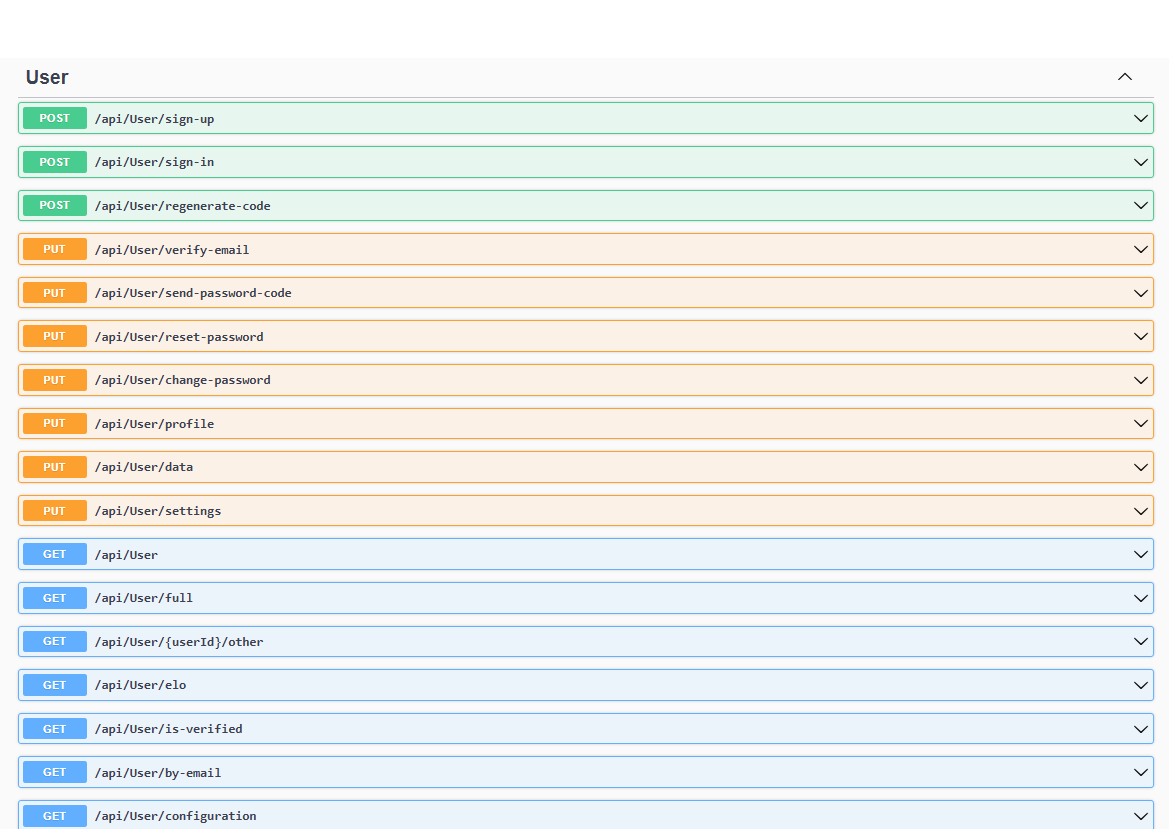
\includegraphics[width=1\textwidth]{zdj/user_controller.png}
        \caption{Punkty końcowe API do rejestracji użytkowników, uwierzytelniania i zarządzania profilami.}
    \end{figure}

    \newpage

    \item \textbf{FriendshipController}
    \begin{itemize} 
        \item \textbf{POST /api/friendship/invite} - Tworzy zaproszenie do znajomości z oczekującym statusem. 
        \item \textbf{POST /api/friendship/block} - Tworzy zaproszenie do znajomości z odrzuconym statusem. 
        \item \textbf{PUT /api/friendship/{friendshipId}/respond} - Zmienia status oczekującej znajomości (akceptacja lub odrzucenie zaproszenia). 
        \item \textbf{GET /api/friendship/all-by-status} - Pobiera wszystkich użytkowników z określonym statusem relacji (np. znajomi, oczekujący). 
        \item \textbf{GET /api/friendship/all-non} - Pobiera wszystkich użytkowników, którzy nie są w relacji z użytkownikiem. 
        \item \textbf{GET /api/friendship/{friendshipId}/profile} - Pobiera profil znajomego na podstawie identyfikatora znajomości. 
        \item \textbf{GET /api/friendship/ranking} - Pobiera ranking użytkowników wśród znajomych na podstawie wybranego modelu. 
        \item \textbf{GET /api/friendship/{friendshipId}/games} - Pobiera listę gier rozegranych w ramach znajomości. 
        \item \textbf{DELETE /api/friendship/{friendshipId}} - Usuwa znajomość i/lub odblokowuje użytkownika. 
    \end{itemize}
    \begin{figure}[h!]
        \centering
        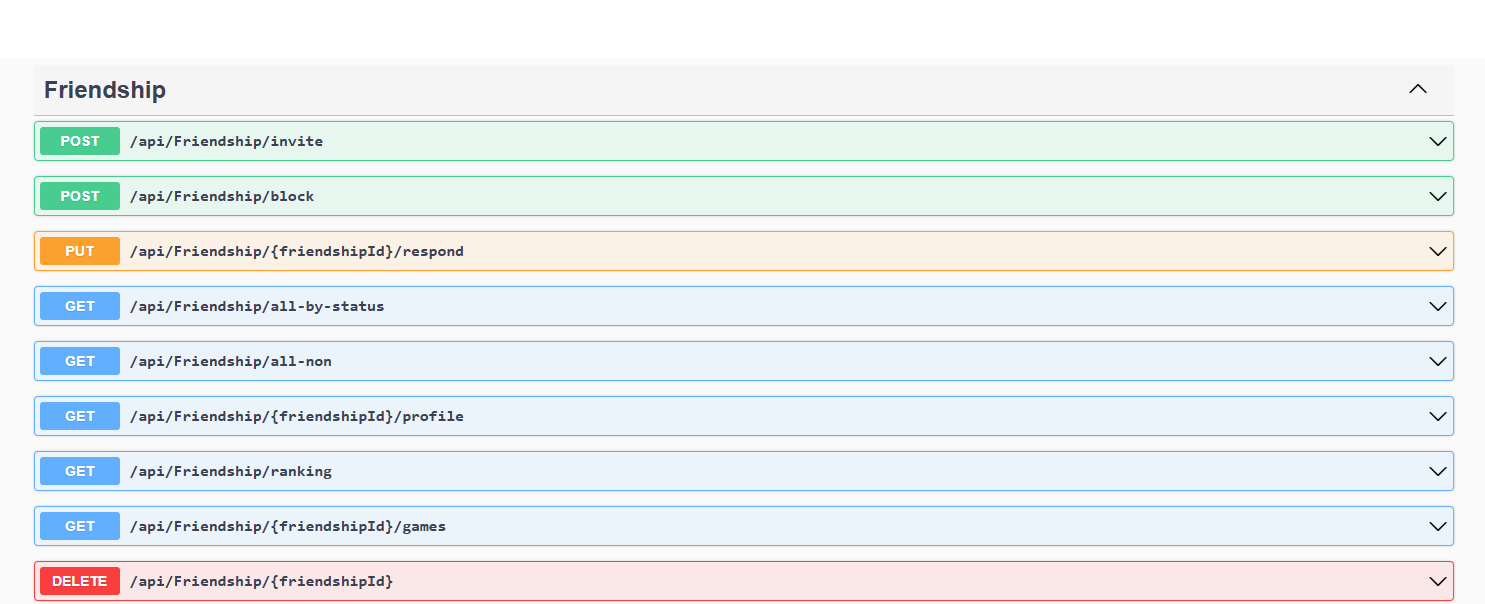
\includegraphics[width=1\textwidth]{zdj/friendship_controller.png}
        \caption{Punkty końcowe API do zarządzania zaproszeniami do znajomych, przyjaźniami i relacjami użytkowników.}
    \end{figure}

    \newpage

    \item \textbf{WebGameController}
    \begin{itemize} 
        \item \textbf{POST /api/webgame/search} - Inicjuje poszukiwanie gry online, tworzy gracza i ustawia czas gry, jeśli nie istnieje. 
        \item \textbf{POST /api/webgame/private} - Tworzy prywatną grę i zwraca jej identyfikator. 
        \item \textbf{POST /api/webgame/email} - Tworzy prywatną grę przez podanie adresu e-mail przeciwnika, zwraca identyfikator gry. 
        \item \textbf{POST /api/webgame/link} - Tworzy prywatną grę z linkiem, który umożliwia dostęp do gry, zwraca identyfikator gry. 
        \item \textbf{GET /api/webgame/is-in-game} - Sprawdza, czy gracz jest już w grze. 
        \item \textbf{GET /api/webgame/{gameId}/update-required} - Sprawdza, czy wymagana jest aktualizacja stanu gry dla gry stworzonej za pomocą linku. 
        \item \textbf{GET /api/webgame/{gameId}} - Pobiera dane jednej gry na podstawie identyfikatora gry. 
        \item \textbf{GET /api/webgame/{gameId}/player} - Pobiera dane gracza w danej grze. 
        \item \textbf{GET /api/webgame/{gameId}/time} - Pobiera czas pozostały dla gracza w danej grze. 
        \item \textbf{GET /api/webgame/{gameId}/opponent} - Pobiera dane przeciwnika z zakończonej gry. 
        \item \textbf{GET /api/webgame/{gameId}/timing} - Pobiera konfigurację czasu gry (timing) dla danej gry. 
        \item \textbf{GET /api/webgame/all-ongoing} - Pobiera wszystkie aktywne gry dla użytkownika. 
        \item \textbf{GET /api/webgame/all-finished} - Pobiera wszystkie zakończone gry dla użytkownika. 
        \item \textbf{GET /api/webgame/type-history} - Pobiera historię gier dla wybranego typu czasu gry. 
        \item \textbf{GET /api/webgame/invitations} - Pobiera wszystkie zaproszenia do gier, które zostały jeszcze nieodebrane. 
        \item \textbf{GET /api/webgame/{gameId}/messages} - Pobiera wszystkie wiadomości z danej gry. 
        \item \textbf{GET /api/webgame/stats} - Pobiera statystyki wszystkich gier rozegranych przez użytkownika. 
        \item \textbf{DELETE /api/webgame/abort} - Anuluje poszukiwanie gry online. 
        \item \textbf{DELETE /api/webgame/{gameId}/cancel} - Anuluje prywatną grę, usuwając graczy. 
    \end{itemize}
    \begin{figure}[h!]
        \centering
        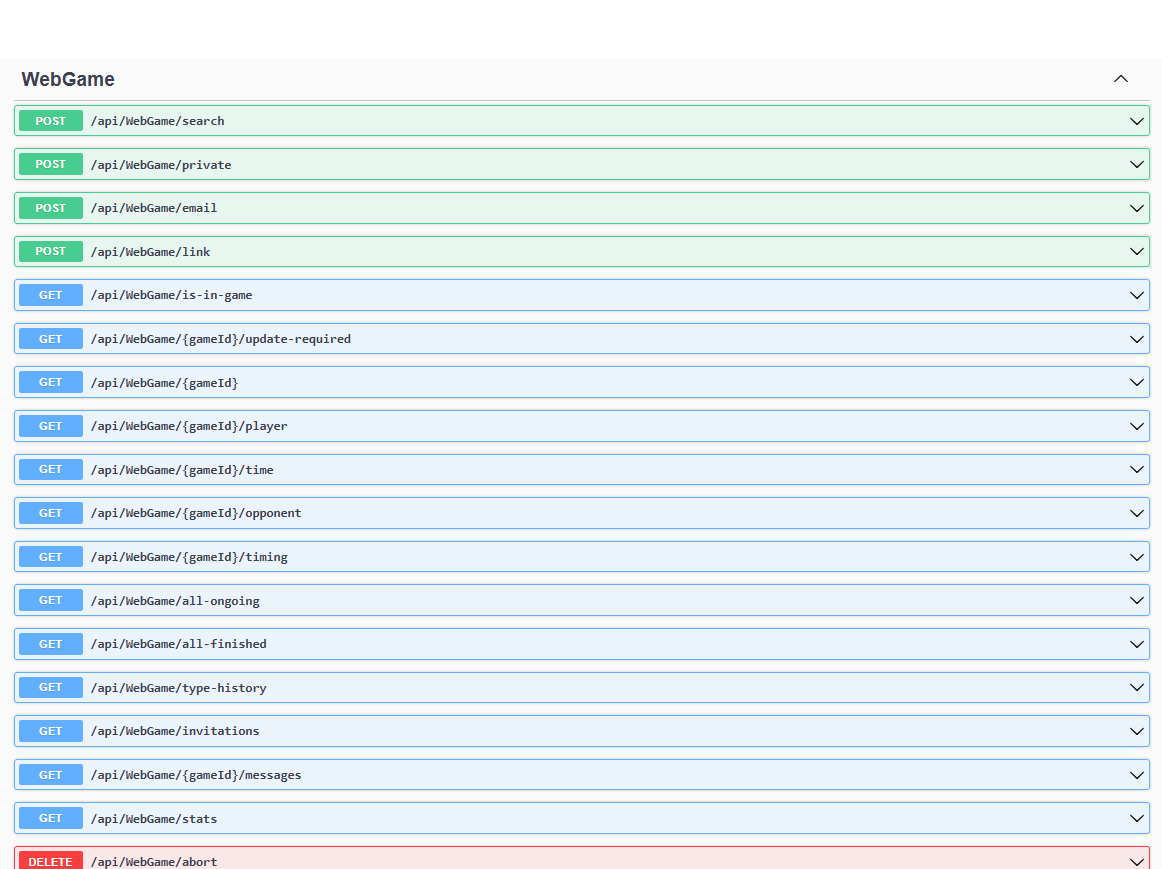
\includegraphics[width=1\textwidth]{zdj/webgame_controller.png}
        \caption{Punkty końcowe API do zarządzania grami sieciowymi, w tym wyszukiwania, tworzenia i sprawdzania statusu graczy w grach publicznych i prywatnych.}
    \end{figure}

    \newpage

    \item \textbf{EngineGameController}
    \begin{itemize} 
        \item \textbf{POST /api/enginegame/start} - Rozpoczyna nową grę z silnikiem szachowym. 
        \item \textbf{POST /api/enginegame/{gameId}/make-move} - Wykonuje ruch w grze, wykonany przez gracza lub silnik.
        \item \textbf{PUT /api/enginegame/{gameId}/end-game} - Kończy grę z silnikiem szachowym. 
        \item \textbf{PUT /api/enginegame/{gameId}/change-engine} - Zmienia poziom trudności silnika szachowego. 
        \item \textbf{PUT /api/enginegame/{gameId}/undo-move} - Cofnięcie ostatniego wykonanego ruchu. 
        \item \textbf{PUT /api/enginegame/update-settings} - Aktualizuje ustawienia związane z grami z silnikiem szachowym. 
        \item \textbf{GET /api/enginegame/{gameId}} - Pobiera wszystkie dane dotyczące gry z silnikiem szachowym.
        \item \textbf{GET /api/enginegame/{gameId}/winner} - Pobiera zwycięzcę gry z silnikiem szachowym. 
        \item \textbf{GET /api/enginegame/{gameId}/engine-move} - Pobiera ruch wykonany przez silnik w grze. 
        \item \textbf{GET /api/enginegame/{gameId}/all-messages} - Pobiera wszystkie wiadomości związane z aktualną grą z silnikiem. 
        \item \textbf{GET /api/enginegame/all-games} - Pobiera wszystkie gry z silnikiem szachowym. 
    \end{itemize}
    \begin{figure}[h!]
        \centering
        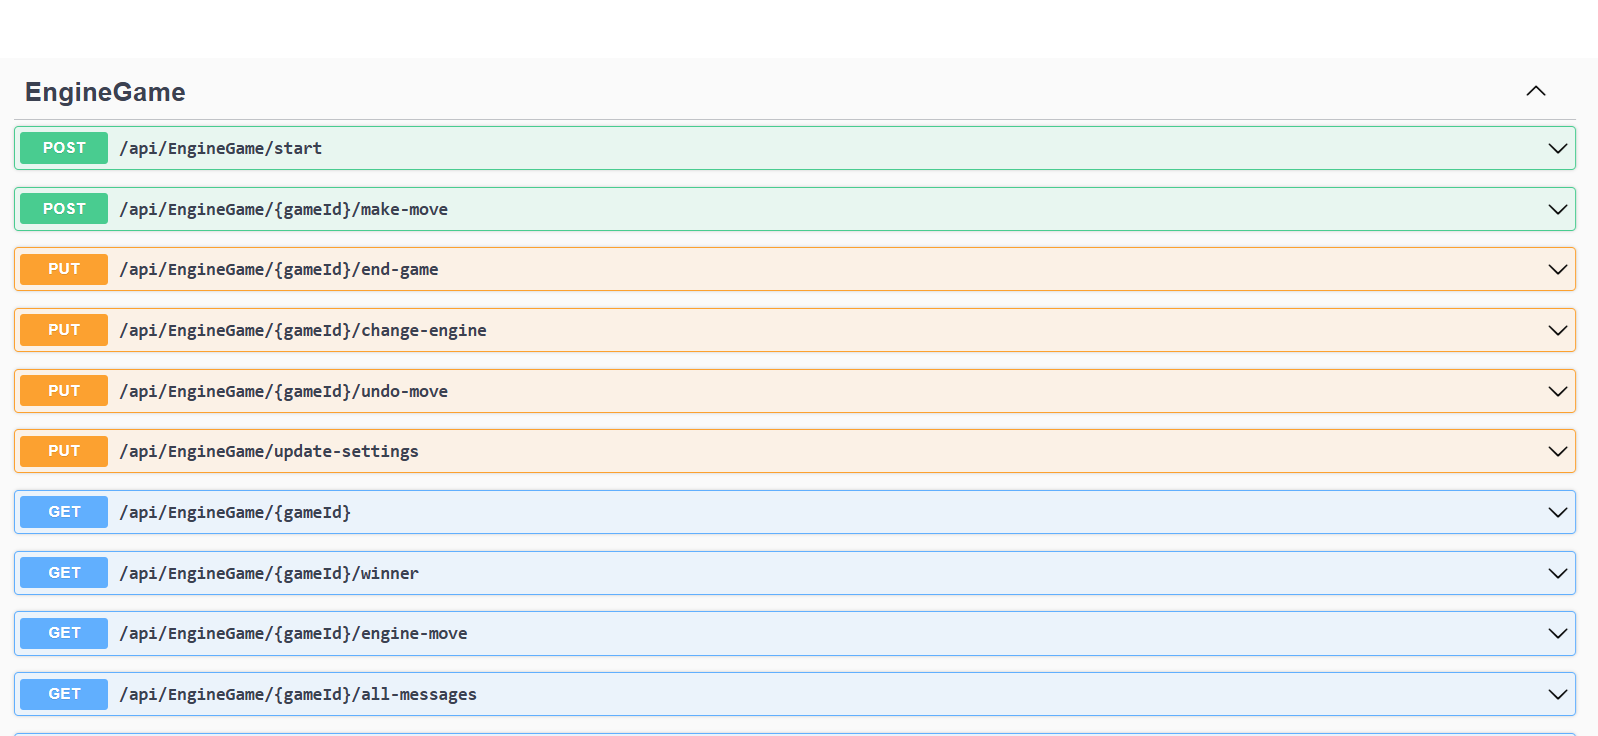
\includegraphics[width=1\textwidth]{zdj/enginegame_controller.png}
        \caption{Punkty końcowe API do zarządzania grami silnika, w tym uruchamiania, wykonywania ruchów, zmiany ustawień i przeglądania danych gry.}
    \end{figure}
\end{itemize}

\newpage
\subsubsection{SignalR}

\newpage
\subsubsection{Komunikacja z silnikiem}
Komunikacja z silnikiem szachowym jest kluczowym elementem w budowie aplikacji, która ma na celu interakcję z popularnymi silnikami szachowymi, takimi jak Stockfish. W przedstawionym przykładzie wykorzystano klasę EngineService, która zapewnia funkcjonalność umożliwiającą komunikację z procesem silnika.

Klasa EngineService implementuje interfejs IEngineService, co zapewnia jednolitość i ułatwia integrację z innymi komponentami aplikacji. W konstruktorze tej klasy tworzony jest obiekt typu Process, który uruchamia silnik szachowy. Proces jest konfigurowany tak, aby nie tworzył okna i umożliwiał przesyłanie danych zarówno do silnika - poprzez standardowe wejście, jak i z silnika - poprzez standardowe wyjście.

\begin{itemize} 
    \item \textbf{Startowanie procesu silnika:} W konstruktorze klasy, obiekt typu Process jest konfigurowany za pomocą klasy ProcessStartInfo. Ustawienia te zapewniają, że silnik będzie działał w tle bez interakcji z interfejsem użytkownika, a komunikacja będzie odbywała się za pomocą strumieni wejścia i wyjścia. 
    \item \textbf{Wysyłanie komend do silnika:} Metoda SendCommand pozwala na wysyłanie komend do silnika. Komendy są przesyłane do standardowego wejścia silnika, a następnie natychmiastowo zapisywane do strumienia wyjściowego. 
    \item \textbf{Odczytywanie wyników:} Metoda ReadOutput służy do odczytywania danych wyjściowych z silnika. Wykorzystuje ona strumień wyjściowy, by zbierać linie tekstu, które są następnie przechowywane w liście. Proces odczytu jest ograniczony czasowo, co zapobiega zablokowaniu aplikacji w przypadku długotrwałych odpowiedzi silnika. 
    \item \textbf{Zamykanie procesu:} Metoda Close wysyła do silnika komendę quit, a następnie zamyka proces, kończąc w ten sposób interakcję z silnikiem. 
\end{itemize}

Dzięki takiej implementacji, aplikacja może komunikować się z silnikiem szachowym w sposób asynchroniczny i kontrolować przebieg gry w czasie rzeczywistym, co jest fundamentem wielu aplikacji szachowych.


\newpage
\subsubsection{Entity Framework Core}


\newpage
\subsection{Frontend}
\subsubsection{Architektura}
Modułowa architektura frontendu
\\\\
Termin ten kładzie nacisk na podział aplikacji na modułowe części wielokrotnego użytku, takie jak "components", "pages", "hooks" i "services". Każdy moduł ma jasny cel, co ułatwia zarządzanie i skalowanie.

\newpage
\subsubsection{Routing aplikacji}

\begin{minted}[fontsize=\small, bgcolor=lightgray]{javascript}
  return (
    <PopupProvider>
      <Routes>
        <Route path="/" element={<IndexPage />} />
        <Route path="/registration" element={<RegisterPage />} />
        <Route path="/about" element={<AboutPage />} />
        <Route path="/about/:contentName" element={<AboutPage />} />
        <Route path="*" element={<NotFoundPage path={"/"} />} />
      </Routes>
    </PopupProvider>
  );
\end{minted}

\begin{minted}[fontsize=\small, bgcolor=lightgray]{javascript}
  return (
    <PopupProvider>
      <Routes>
        <Route path="/" element={<MainPage />} />
        <Route path="/users" element={<UsersPage />} />
        <Route path="/await/:gameIdStr" element={<AwaitingPage />} />
        <Route path="/game/:gameIdStr" element={<WebGamePage />} />
        <Route path="/engine-game/:gameIdStr" element={<EngineGamePage />} />
        <Route path="/account" element={<AccountPage />} />
        <Route path="/profile/:friendshipIdStr" element={<ProfilePage />} />
        <Route path="/ranking" element={<RankingPage />} />
        <Route path="*" element={<NotFoundPage path={"/main"} />} />
      </Routes>
    </PopupProvider>
  );
\end{minted}

\newpage

\begin{minted}[fontsize=\small, bgcolor=lightgray]{javascript}
    useEffect(() => {
        const verifyUsersToken = async (): Promise<void> => {
        const path = location.pathname;

        try {
            const token = localStorage.getItem("token");
            if (!token) {
            const state: StateOptions = /* details omitted */;

            navigate("/registration", { state: state, replace: true });
            return;
            }

            const response = await axios.get<IsEmailVerifiedDto>(
                userController.isVerified(), getAuthorization());

            const isVerified = response.data.isEmailVerified;
            if (!isVerified) {
            const state: StateOptions = /* details omitted */;

            navigate("/registration", { state: state, replace: true });
            return;
            }

            const userInfoResponse = await axios.get<GetUserDto>(
                userController.getUser(), getAuthorization());
            localStorage.setItem("userInfo", JSON.stringify(userInfoResponse.data));

            await GameHubService.startConnectionWithToken(token);

            if (GameHubService.connection?.state === HubConnectionState.Connected) {
            await GameHubService.AddSelfNotification();

            setAuthorize(true);
            }
        } catch (err) {
            const state: StateOptions = /* details omitted */;

            navigate("/registration", { state: state });
        }
        };

        verifyUsersToken();
    }, []);
\end{minted}
            
\newpage
\subsubsection{Wykorzystane biblioteki}

\begin{itemize}
    \item \textbf{@microsoft/signalr}: Biblioteka SignalR od Microsoftu pozwala na komunikację w czasie rzeczywistym między aplikacjami frontendowymi a serwerem. Jest to kluczowa biblioteka, umożliwiająca implementację funkcji czatu lub powiadomień w czasie rzeczywistym, np. w grze szachowej, w której użytkownicy mogą odbierać i wysyłać wiadomości na żywo.
    \item \textbf{@mui/x-charts}: Biblioteka wykorzystywana do tworzenia interaktywnych wykresów i wizualizacji danych w aplikacjach React. Może być używana do wyświetlania analiz, statystyk lub wyników gier w postaci wykresów.
    \item \textbf{@types/jsonwebtoken}: Typy TypeScript dla biblioteki jsonwebtoken. Używane do pracy z tokenami JWT (JSON Web Tokens), które mogą być wykorzystywane do uwierzytelniania i autoryzacji użytkowników w aplikacjach webowych.
    \item \textbf{axios}: Klient HTTP, który ułatwia wykonywanie zapytań do API. Jest to popularne narzędzie do pracy z zapytaniami typu GET, POST, PUT, DELETE i innymi, pozwalające na łatwą obsługę odpowiedzi z serwera, w tym błędów.
    \item \textbf{guid-typescript}: Biblioteka umożliwiająca generowanie i operowanie na identyfikatorach GUID (Globally Unique Identifiers) w aplikacjach TypeScript. Może być używana do generowania unikalnych identyfikatorów, np. dla nowych gier, użytkowników lub sesji.
    \item \textbf{history}: Biblioteka zarządzająca historią przeglądarki, używana przez react-router-dom do zarządzania nawigacją w aplikacjach SPA (Single Page Application). Pozwala na manipulowanie historią przeglądarki (np. przechodzenie do nowych stron bez przeładowania strony).
    \item \textbf{jsonwebtoken}: Biblioteka do tworzenia i weryfikacji tokenów JWT. JWT jest szeroko stosowanym standardem w aplikacjach webowych do zarządzania uwierzytelnianiem i autoryzacją użytkowników.
    \item \textbf{jwt-decode}: Biblioteka do dekodowania tokenów JWT. Pomaga w ekstrakcji informacji z tokenów, takich jak dane użytkownika lub czas wygaśnięcia tokenu.
    \item \textbf{msw}: Mock Service Worker – biblioteka służąca do tworzenia fikcyjnych serwisów (mocking API). Używana do testowania aplikacji frontendowych bez konieczności posiadania aktywnego backendu. Może służyć do mockowania odpowiedzi z API w trakcie rozwoju lub testów.
    \item \textbf{react}: Podstawowa biblioteka do budowy interfejsów użytkownika w aplikacjach frontendowych. React jest wykorzystywany do tworzenia dynamicznych komponentów UI, które mogą się aktualizować w odpowiedzi na zmiany w danych.
    \item \textbf{react-dom}: Zawiera funkcje do renderowania aplikacji React na stronie HTML. Jest to kluczowy komponent w ekosystemie React, umożliwiający integrację z DOM.
    \item \textbf{react-router-dom}: Biblioteka do obsługi routingu w aplikacjach React. Umożliwia tworzenie linków, trasowanie i zarządzanie nawigacją między różnymi widokami (stronami) w aplikacji SPA.
    \item \textbf{sass}: Preprocesor CSS, który pozwala na pisanie bardziej zorganizowanego i modularnego CSS. Zawiera funkcje takie jak zmienne, zagnieżdżanie, mixiny, które ułatwiają pisanie i utrzymanie kodu stylów.
    \item \textbf{scss}: Skrócona nazwa dla SASS (Syntactically Awesome Stylesheets). SCSS to rozszerzenie składni SASS, które jest bardziej zbliżone do standardowego CSS i jest szeroko stosowane w nowoczesnych aplikacjach frontendowych.
    \item \textbf{uuid}: Biblioteka do generowania unikalnych identyfikatorów UUID. Jest często używana w aplikacjach do generowania identyfikatorów dla elementów lub sesji.
    \item \textbf{@eslint/js}: Biblioteka ESLint dla JavaScript, wykorzystywana do sprawdzania jakości kodu, wychwytywania błędów i utrzymywania spójnego stylu kodowania w zespole.
    \item \textbf{@testing-library/dom}: Biblioteka do testowania DOM w aplikacjach frontendowych, pozwala na tworzenie testów jednostkowych i integracyjnych w React.
    \item \textbf{@testing-library/react}: Biblioteka wspomagająca testowanie komponentów React, która integruje się z popularnymi narzędziami do testów, takimi jak Jest i React Testing Library.
    \item \textbf{eslint}: Narzędzie do statycznej analizy kodu, wykorzystywane do zapewnienia jakości i spójności kodu JavaScript/TypeScript, zgodnie z określonymi zasadami.
    \item \textbf{stylelint}: Narzędzie do analizy CSS i SCSS, które pomaga w utrzymaniu porządku i jakości kodu stylów.
    \item \textbf{typescript}: Typowanie statyczne dla JavaScriptu. TypeScript dodaje do JavaScript typy i inne funkcje, które pomagają uniknąć błędów w kodzie i poprawiają skalowalność aplikacji.
    \item \textbf{vite}: Szybki bundler i serwer deweloperski, który wspiera nowoczesne technologie, takie jak ES Modules, TypeScript i React, zapewniając szybki czas ładowania podczas pracy nad projektem.
    \item \textbf{vitest}: Framework do testowania w ekosystemie Vite. Umożliwia szybkie uruchamianie testów jednostkowych, które są zgodne z biblioteką Jest, ale zoptymalizowane pod kątem Vite.
\end{itemize}

\newpage
\section{Instrukcja obsługi}

\subsection{Strona startowa}
Strona tytułowa aplikacji do gry w szachy została zaprojektowana jako intuicyjny i funkcjonalny punkt startowy dla użytkowników. Umieszczono na niej wszystkie kluczowe elementy, które pozwalają na łatwe rozpoczęcie korzystania z platformy. W górnej części strony znajdują się przyciski umożliwiające logowanie oraz rejestrację, co pozwala zarówno nowym użytkownikom, jak i tym posiadającym konto na szybki dostęp do zasobów aplikacji.
\\\\
Centralna część strony prezentuje krótki opis funkcjonalności aplikacji. Zwrócono uwagę na najważniejsze elementy, takie jak możliwość gry online z innymi użytkownikami, rozbudowane narzędzia treningowe, tryb rozwiązywania łamigłówek szachowych oraz funkcje organizowania i uczestnictwa w turniejach. Wszystko to ma na celu wprowadzenie użytkownika w możliwości, jakie oferuje aplikacja, oraz zachęcenie do eksplorowania dostępnych funkcji.
\\\\
Na stronie znajduje się również sekcja umożliwiająca przejście do bardziej szczegółowego opisu zawartości aplikacji. Dzięki niej można zapoznać się z opisem poszczególnych funkcji oraz dowiedzieć się więcej o opcjach gry i trybach nauki. Dodatkowo zamieszczono odnośnik do działu FAQ, w którym zebrano odpowiedzi na najczęściej zadawane pytania, ułatwiając użytkownikom szybkie rozwiązanie ewentualnych wątpliwości.
\\\\
Całość zaprojektowano w sposób przejrzysty i estetyczny, aby zapewnić pozytywne pierwsze wrażenie oraz łatwość w poruszaniu się po stronie. Strona tytułowa pełni rolę wizytówki aplikacji, jednocześnie oferując dostęp do najważniejszych zasobów i funkcji.

\begin{figure}[h!]
    \centering
    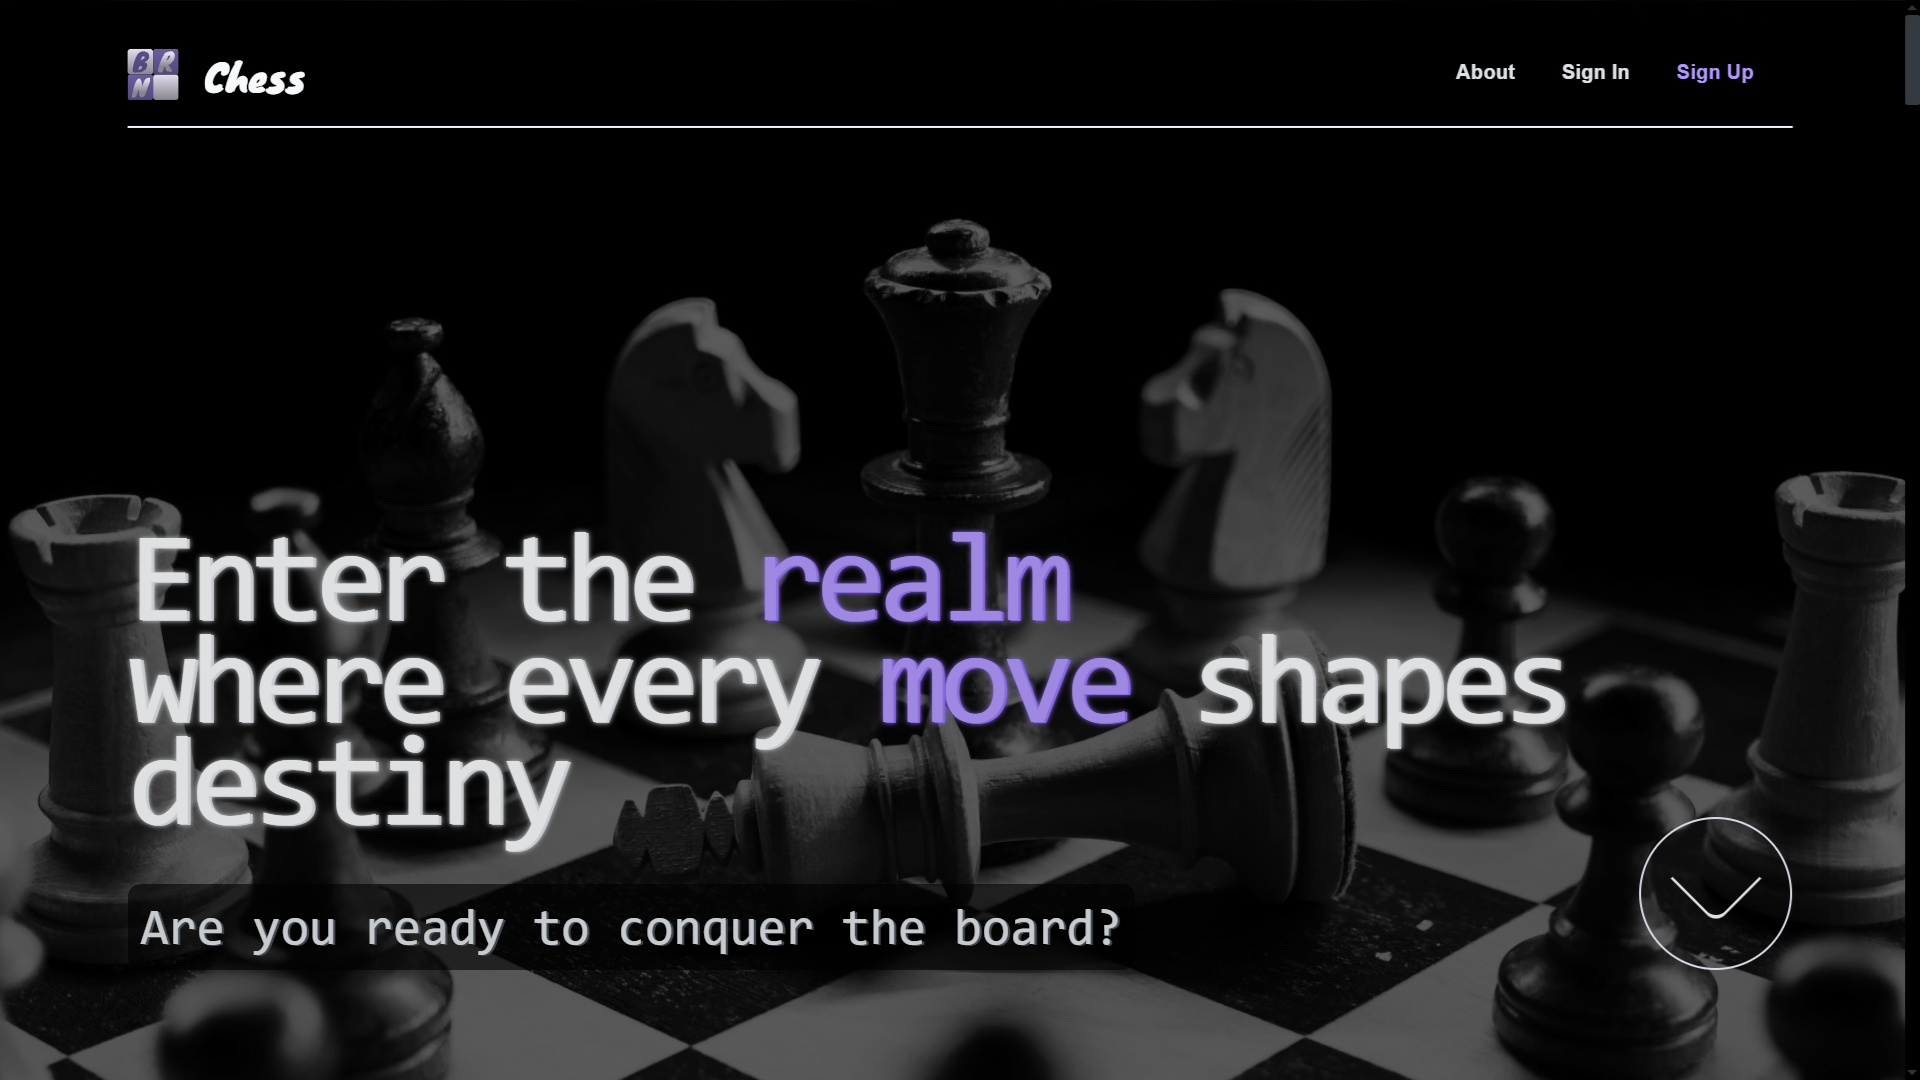
\includegraphics[width=1\textwidth]{zdj/ins_hero.png}
    \caption{Widok strony startowej.}
\end{figure}

\newpage
\subsection{Strona rejestracji}
Strona rejestracji w aplikacji łączy w sobie wszystkie kluczowe funkcje niezbędne do zarządzania kontem użytkownika. Pozwala na założenie nowego profilu, zalogowanie się na istniejące konto, odzyskanie dostępu w przypadku utraty hasła oraz potwierdzenie adresu e-mail jako element weryfikacji konta. Wszystkie te opcje zostały zaprojektowane w sposób intuicyjny i łatwy w obsłudze, aby zapewnić jak najlepsze doświadczenie użytkownika.
\\\\
Proces rejestracji umożliwia szybkie i bezproblemowe utworzenie konta. Po podaniu podstawowych danych, takich jak adres e-mail, nawa użytkownika oraz hasło, użytkownik otrzymuje wiadomość e-mail z linkiem aktywacyjnym, który potwierdza poprawność podanych informacji i zabezpiecza konto przed nieautoryzowanym dostępem. Logowanie do istniejącego konta odbywa się poprzez wprowadzenie e-maila lub nazwy uzytkownika i hasła.
\\\\
W przypadku zapomnianego hasła, strona oferuje funkcję jego odzyskania. Po podaniu adresu e-mail użytkownik otrzymuje szczegółowe instrukcje dotyczące resetowania hasła, co pozwala w bezpieczny sposób odzyskać dostęp do konta. Proces jest prosty i zabezpieczony dodatkowymi krokami weryfikacyjnymi.

\begin{figure}[h!]
    \centering
    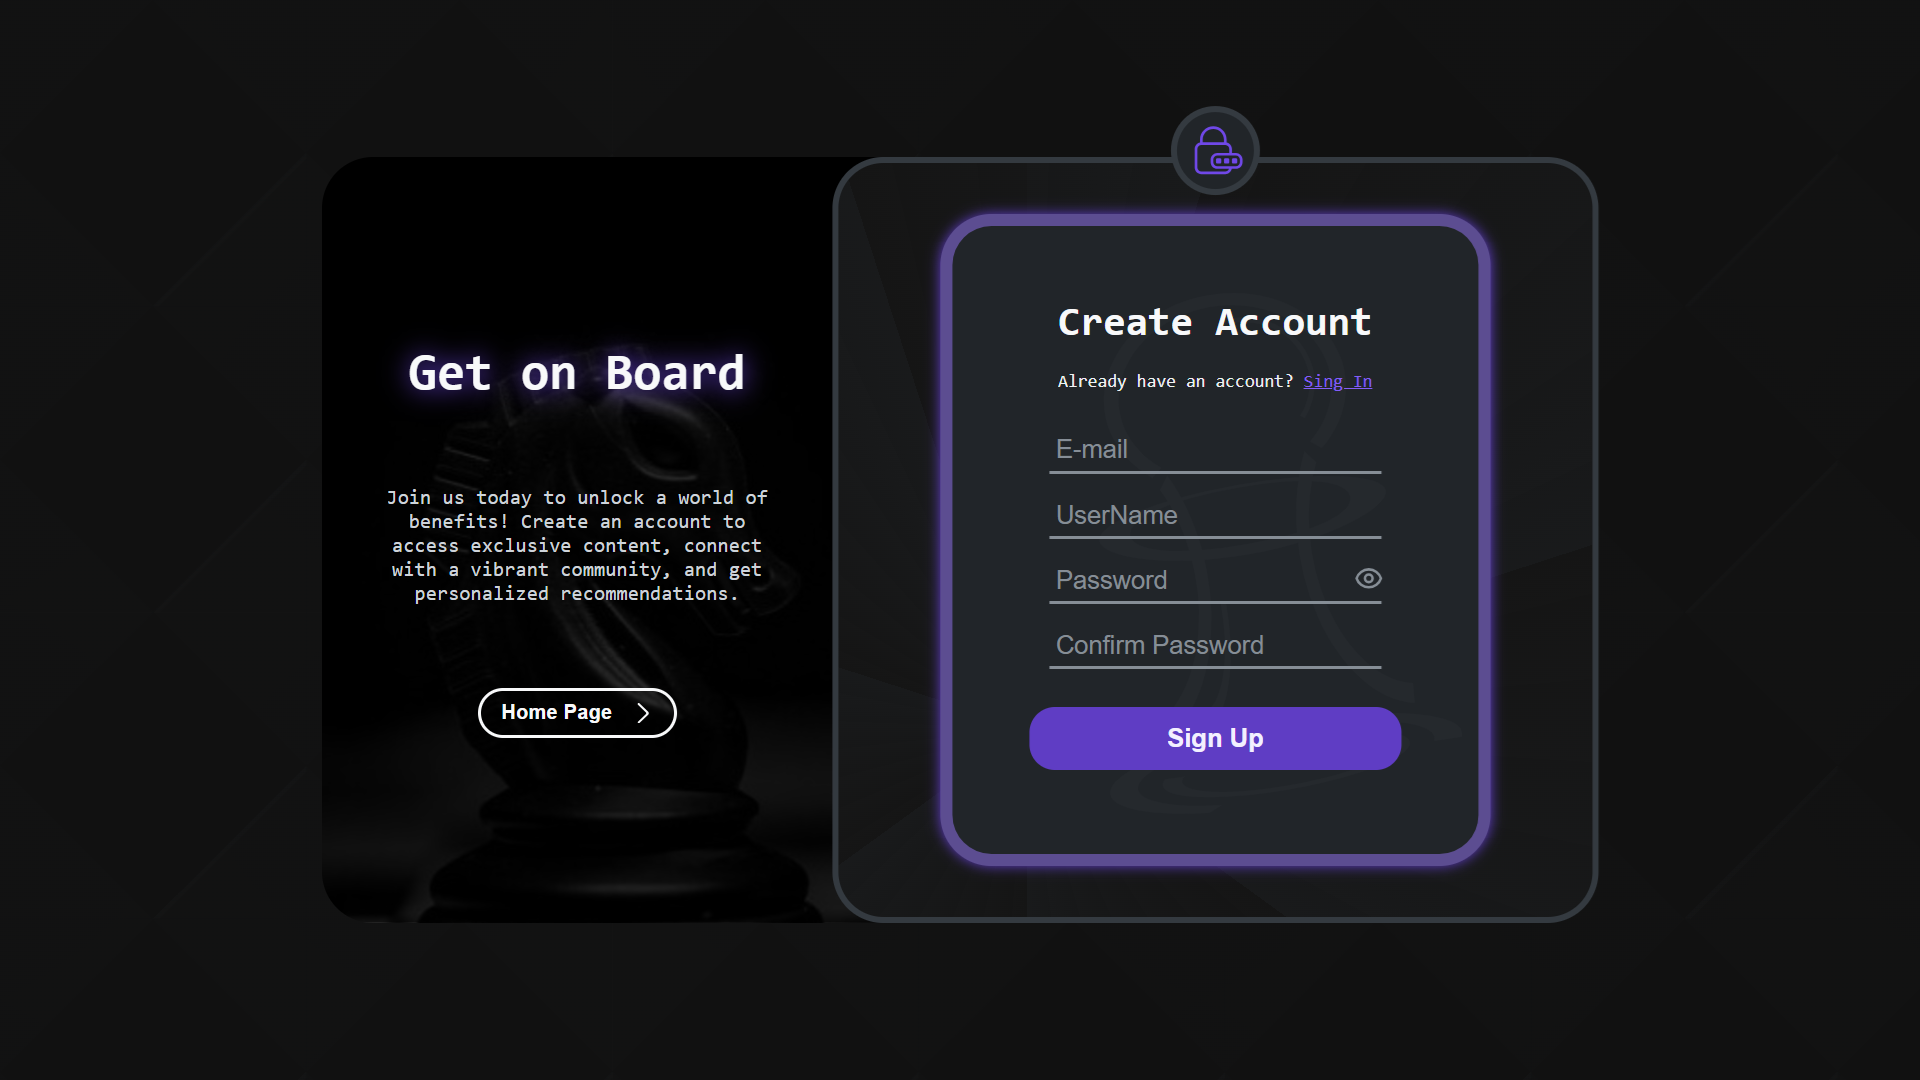
\includegraphics[width=1\textwidth]{zdj/ins_reg.png}
    \caption{Widok strony startowej.}
\end{figure}

Strona rejestracji jest zaprojektowana z myślą o czytelności i łatwości obsługi, dzięki czemu użytkownicy mogą bez przeszkód korzystać z jej funkcji niezależnie od poziomu zaawansowania. Wszystkie kroki są jasno opisane, a interfejs dostosowano do potrzeb zarówno nowych, jak i stałych użytkowników aplikacji.

\newpage
\subsection{Weryfikacja konta}

\begin{minipage}[t]{0.45\textwidth} 
    \vspace{0pt} 
    \raggedright Weryfikacja konta to jeden z kluczowych etapów rejestracji, mający na celu zapewnienie bezpieczeństwa danych użytkowników oraz ochronę przed nieuprawnionym dostępem. Po zakończeniu procesu rejestracji aplikacja automatycznie generuje wiadomość e-mail, która zawiera wszystkie informacje niezbędne do ukończenia weryfikacji. System weryfikacyjny nie tylko wspiera proces zakładania konta, ale również jest wykorzystywany przy odzyskiwaniu hasła, co zapewnia spójność działania i zwiększa bezpieczeństwo użytkowników. 
\end{minipage} 
\hfill 
\begin{minipage}[t]{0.45\textwidth} 
    \vspace{0pt} 
    \centering 
    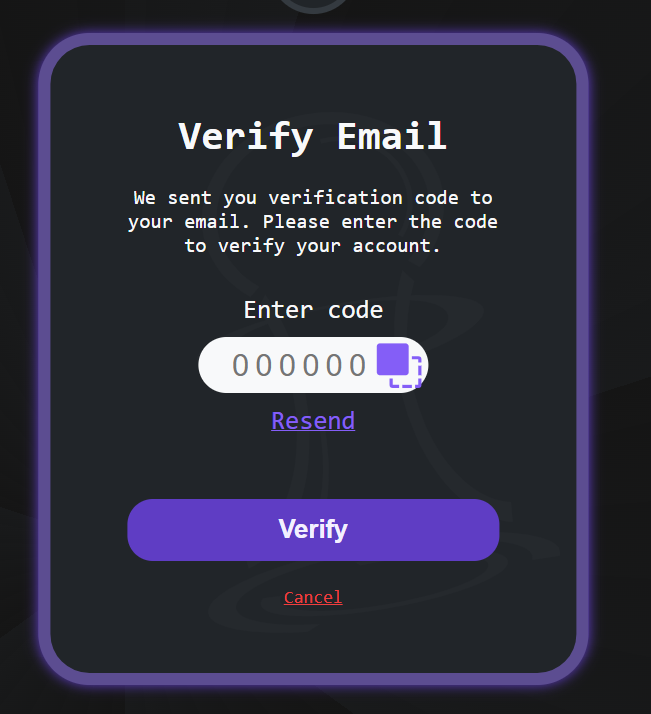
\includegraphics[width=\linewidth]{zdj/ins_min_ver.png} 
\end{minipage}

\vspace{1cm}

\begin{minipage}[t]{0.45\textwidth} 
    \vspace{0pt} 
    \centering 
    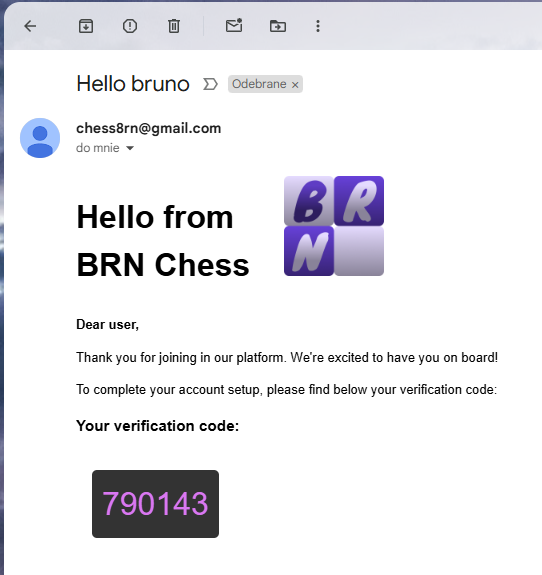
\includegraphics[width=\linewidth]{zdj/ins_min_mail.png} 
\end{minipage} 
\hfill 
\begin{minipage}[t]{0.45\textwidth} 
    \vspace{0pt} 
    \raggedright Wiadomość e-mail, zatytułowana "Hello from BRN Chess", zawiera przyjazne powitanie, a także unikalny kod weryfikacyjny przypisany do konkretnego konta użytkownika. Treść e-maila została zaprojektowana tak, aby była czytelna i estetyczna, co pozwala na szybkie odnalezienie wymaganych informacji. Kod weryfikacyjny, przedstawiony w formie wyróżnionego tekstu, należy skopiować i wkleić w dedykowane pole tekstowe w oknie weryfikacji w aplikacji. Po wprowadzeniu kodu i jego zatwierdzeniu konto zostaje w pełni aktywowane, a użytkownik może rozpocząć korzystanie z platformy. 
\end{minipage}

\vspace{1cm}

Cały proces został opracowany z myślą o wygodzie użytkownika. Okno weryfikacyjne w aplikacji jest intuicyjne, zawiera czytelne instrukcje oraz widoczne przyciski umożliwiające wprowadzenie kodu. Dodatkowo w przypadku problemów, takich jak brak dostarczenia wiadomości e-mail, aplikacja oferuje możliwość ponownego wysłania kodu weryfikacyjnego za pomocą jednego kliknięcia.
\\\\
Weryfikacja konta to proces szybki i bezproblemowy, a dzięki jasnym instrukcjom użytkownicy mogą sprawnie zakończyć konfigurację swojego konta i skupić się na odkrywaniu możliwości aplikacji.

\newpage
\subsection{Strona główna}
Strona główna aplikacji szachowej została zaprojektowana z myślą o intuicyjnej nawigacji i szybkim dostępie do kluczowych funkcji, aby zapewnić użytkownikom wygodę i efektywność. Po prawej stronie ekranu znajduje się pasek nawigacji, który umożliwia łatwe przechodzenie między różnymi stronami aplikacji, zapewniając dostęp do wszystkich istotnych sekcji. Pasek został umieszczony w widocznym miejscu, dzięki czemu poruszanie się po aplikacji jest szybkie i płynne.
\\\\
Obok paska nawigacji umieszczono główne przyciski, które prowadzą do najważniejszych funkcji aplikacji. Każdy z nich odpowiada za inną czynność:
\begin{itemize}
    \item \textbf{Gra online:} umożliwia rozpoczęcie partii z innym graczem przez internet.
    \item \textbf{Gra z komputerem:} pozwala zmierzyć się z silnikiem szachowym.
    \item \textbf{Gra ze znajomymi:} umożliwia zapraszanie znajomych do wspólnej gry.
    \item \textbf{Wgląd w gry użytkownika:} pokazujące zakończone jak i wciąż trwające partie.
    \item \textbf{Zaproszenia do gier:} wyświetla listę otrzymanych zaproszeń do rozgrywek.
\end{itemize}

Pozostałą przestrzeń zajmują okna szybkiego dostępu, takie jak podgląd konta użytkownika, szybka gra online z wyborem trzech trybów czasowych (1 min, 3 min, 10 min), a także widok trzech ostatnich zakończonych i trzech aktywnych gier. Całość jest intuicyjna, zapewniając wygodne korzystanie z aplikacji.

\begin{figure}[h!]
    \centering
    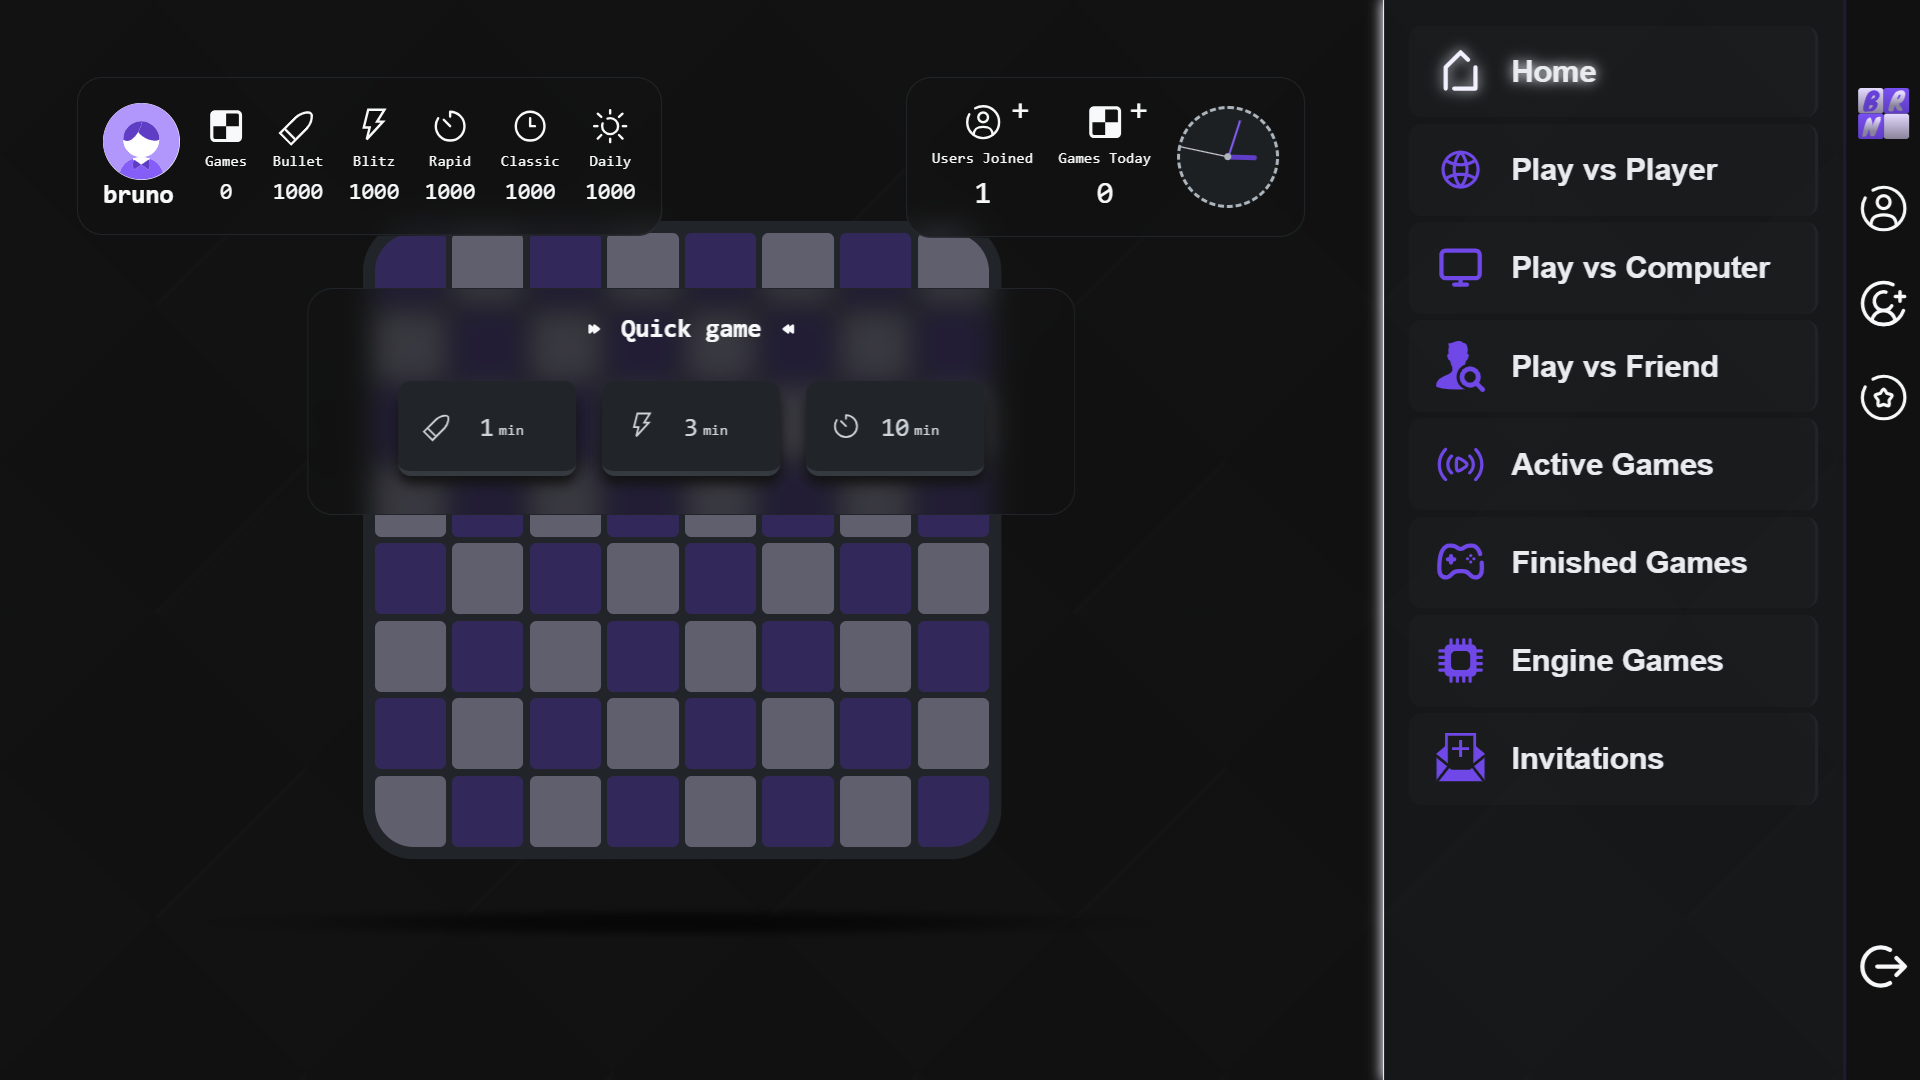
\includegraphics[width=1\textwidth]{zdj/ins_main.png}
    \caption{Widok strony głównej.}
\end{figure}

\newpage
\subsection{Gra online}
Po kliknięciu na przycisk gry online, użytkownik zostaje przeniesiony do okna, które pozwala na wybór odpowiedniego trybu kontroli czasowej dla gry. W zależności od preferencji, dostępne są różne opcje czasowe, zgrupowane w kategorie, takie jak bullet, blitz, rapid, classic oraz daily.
\\\\
W sekcji bullet użytkownik ma do wyboru bardzo szybkie tryby, takie jak 1 minuta bez dodatkowego czasu (1min), z dodatkowymi sekundami (1m|1s), lub 2 minuty z opcją 1 sekundy dodatkowego czasu (2m|1s). Dla blitz oferowane są opcje 3 minuty, 3 minuty z 5 sekundami dodatkowego czasu, 5 minut, oraz 5 minut z 10 sekundami dodatkowymi. W przypadku rapid dostępne są opcje 10 minut, 15 minut oraz 30 minut. Tryby classic pozwalają na bardzo długie partie z czasem od 1 godziny do 5 godzin, w zależności od preferencji gracza. Ostatnia kategoria, daily, oferuje najbardziej rozciągnięte w czasie partie, gdzie każdy gracz ma od 1 do 30 dni na rozegranie partii.
\\\\
Po dokonaniu wyboru jednego z powyższych trybów, ekran zmienia się na widok wyszukiwania przeciwnika. W tym momencie system zaczyna szukać dostępnego gracza o podobnym czasie reakcji, aby rozpocząć rozgrywkę. Użytkownik może na bieżąco śledzić postęp tego procesu, a po znalezieniu przeciwnika następuje połączenie i rozpoczęcie gry.

\begin{figure}[h!]
    \centering
    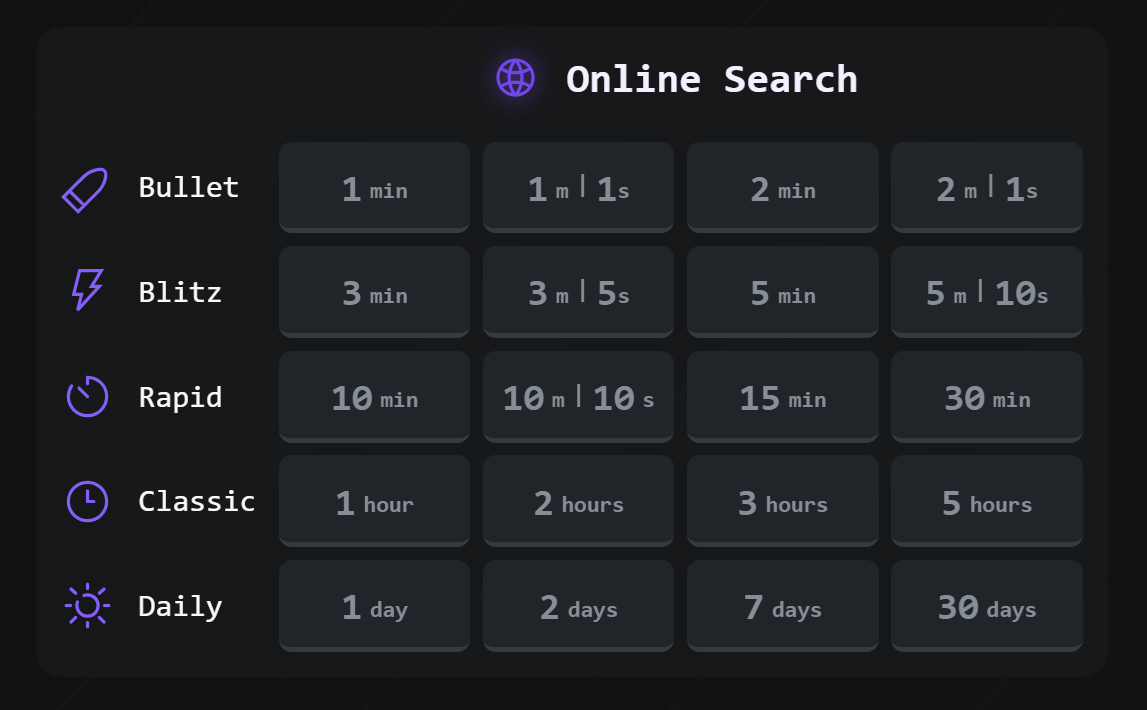
\includegraphics[width=1\textwidth]{zdj/ins_min_pvp.png}
    \caption{Widok wyboru gry online.}
\end{figure}

\newpage
\subsection{Gra offline}
Po kliknięciu na przycisk "Gra z komputerem", użytkownik zostaje poproszony o wybór poziomu trudności silnika. Istnieje 20 poziomów, które symbolicznie podzielono na cztery kategorie: standard, intermediate, advanced oraz master. Należy jednak podkreślić, że podział ten ma charakter jedynie orientacyjny i nie wpływa w żaden sposób na faktyczny sposób działania silnika. Jest to tylko sposób ułatwiający użytkownikowi poruszanie się po dostępnych opcjach, a wybór konkretnego poziomu zależy od indywidualnych preferencji gracza.
\\\\
Po dokonaniu wyboru poziomu silnika gra uruchamia się natychmiastowo, a użytkownik może zacząć rywalizować z komputerowym przeciwnikiem. Warto dodać, że w przypadku gry z komputerem nie ma zastosowanej kontroli czasowej, co oznacza, że gracz może spokojnie analizować ruchy bez presji czasu.
\\\\
Dodatkowo, podczas gry z komputerem istnieje opcja oszukiwania, czyli możliwość cofania ruchów lub zmiany poziomu silnika w trakcie rozgrywki. Ta funkcja daje graczowi elastyczność i pozwala na dostosowanie poziomu trudności w trakcie gry, jeśli uzna to za konieczne. Opcja ta jest jednak dostępna tylko w tej formie w grze z komputerem. Użytkownik może także zmienić preferencje dotyczące oszukiwania, a także inne ustawienia, na stronie swojego profilu, którą opisujemy w dalszej części instrukcji.

\begin{figure}[h!]
    \centering
    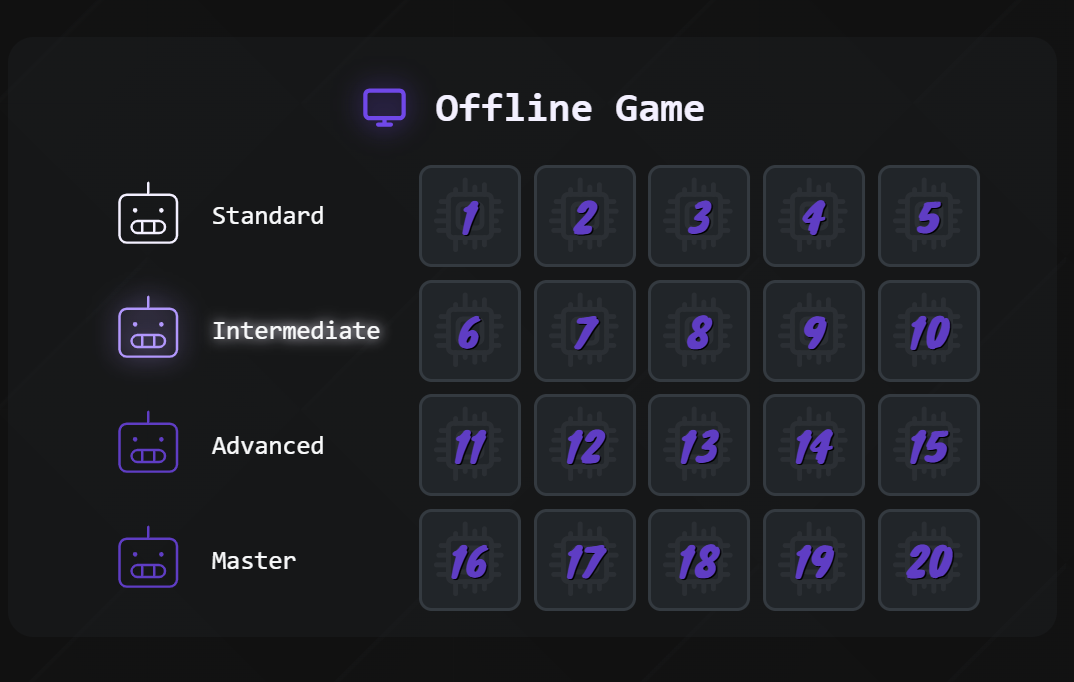
\includegraphics[width=1\textwidth]{zdj/ins_min_pvc.png}
    \caption{Widok wyboru gry offline.}
\end{figure}

\newpage
\subsection{Gra ze znajomymi}
Po kliknięciu na przycisk „Gra ze znajomymi”, użytkownik zostaje przeniesiony do okna, gdzie po lewej stronie znajduje się opcje zapraszania do gry, a po prawej widoczna jest lista wszystkich znajomych, którzy mają konto w aplikacji. Po kliknięciu na kartę znajomego użytkownik zostaje przekierowany do ekranu wyboru czasu gry, podobnie jak w przypadku gry online z losowym przeciwnikiem, gdzie wybiera się jedną z dostępnych opcji czasowych. Po dokonaniu wyboru czasu, gra natychmiast przechodzi do strony oczekiwania na dołączenie drugiego gracza, użytkownik będzie czekał, aż zaproszona osoba zaakceptuje zaproszenie i dołączy do gry.
\\\\


\begin{figure}[h!]
    \centering
    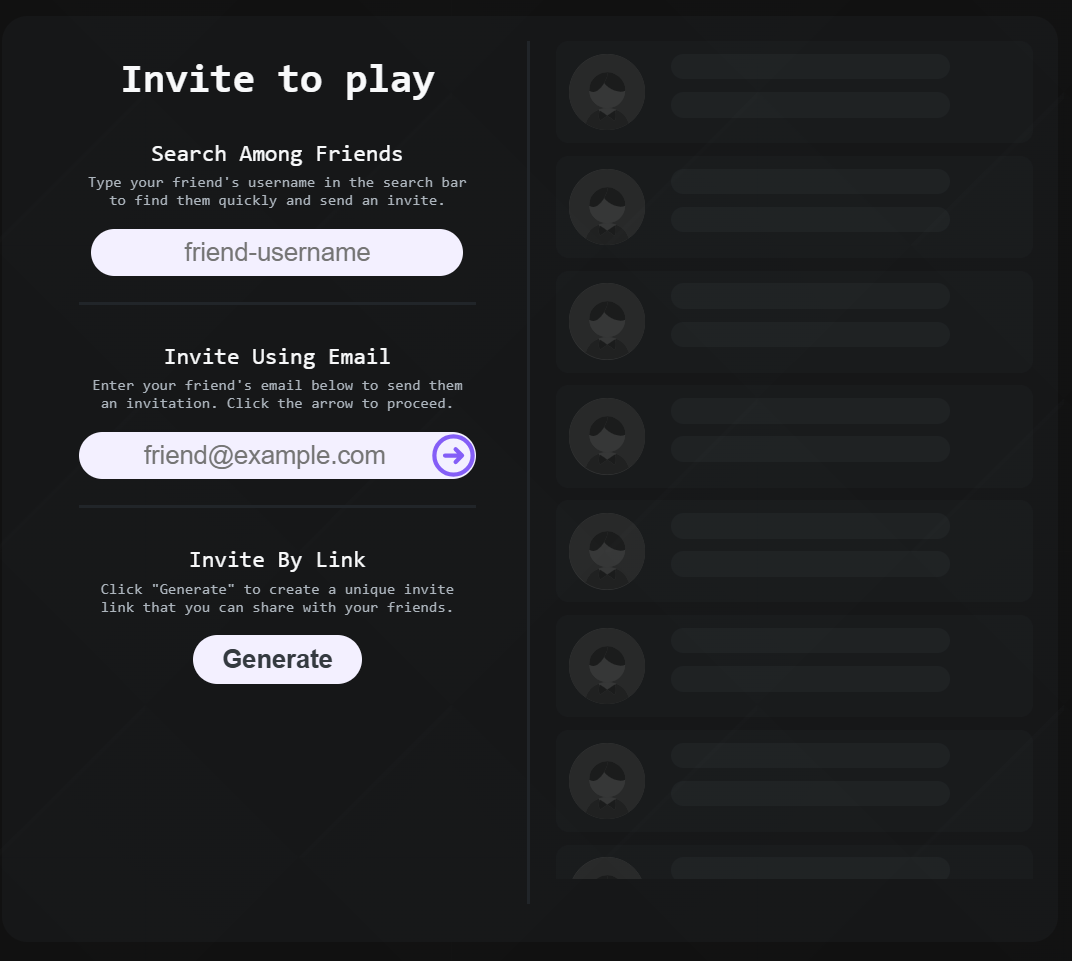
\includegraphics[width=1\textwidth]{zdj/ins_min_pvf.png}
    \caption{Widok wyboru gry ze znajomym.}
\end{figure}

\newpage

Po prawej stronie ekranu znajdują się trzy główne opcje umożliwiające zapraszanie do gry. Pierwsza z nich pozwala na filtrowanie znajomych po nazwie użytkownika. Dzięki temu, w przypadku długiej listy znajomych, łatwiej można znaleźć konkretnego gracza. Druga opcja to bezpośrednie zaproszenie przez e-mail. Po podaniu prawidłowego adresu e-mail użytkownik zostaje przekierowany do wyboru czasu gry, tak jak ma to miejsce w przypadku zapraszania znajomego z listy. Jeśli jednak wprowadzony adres e-mail jest niepoprawny lub nie istnieje w systemie, aplikacja wyświetli komunikat informujący, że taki użytkownik nie istnieje. Dzięki tej funkcji użytkownicy mogą zapraszać do gry nie tylko swoich znajomych, ale także osoby spoza listy znajomych, wystarczy, że podadzą poprawny adres e-mail. Jeśli podany adres jest prawidłowy i istnieje w systemie, zaproszenie zostaje wysłane, a użytkownik zostaje przekierowany do wyboru czasu gry.
\\\\
Trzecia opcja, „Gra za pomocą wygenerowanego linka”, pozwala na zaproszenie do gry gracza, który nie jest bezpośrednio na liście znajomych. Po dokonaniu wyboru kontroli czasowej, wyświetla się zmodyfikowane okno oczekiwania, w którym pojawi się unikalny link. Link ten jest kluczowy dla całej procedury – to za jego pomocą zapraszający gracz będzie mógł zaprosić innego użytkownika do dołączenia do gry. W celu rozpoczęcia gry, zapraszający użytkownik musi skopiować wygenerowany link i wysłać go znajomemu za pomocą dowolnego komunikatora, na przykład e-maila, messengera lub innej aplikacji. Po kliknięciu w link przez zaproszonego gracza, następuje przekierowanie na specjalną stronę, która automatycznie dołączy tego gracza do gry. Kiedy obaj gracze wejdą na tę stronę, będą przekierowani do samej gry, gdzie rozgrywka się rozpocznie. Jeśli jednak zapraszający kliknie w link, aby dołączyć do gry, otrzyma komunikat o błędzie, ponieważ nie może dołączyć do własnej gry. System wyświetli informację, że musi to być inny gracz, który kliknie w link, aby rozpocząć rozgrywkę. Dzięki temu proces zapraszania i dołączania do gry jest prosty, a użytkownik zapraszający ma pełną kontrolę nad wysłaniem linku do odpowiedniej osoby.

\begin{figure}[h!]
    \centering
    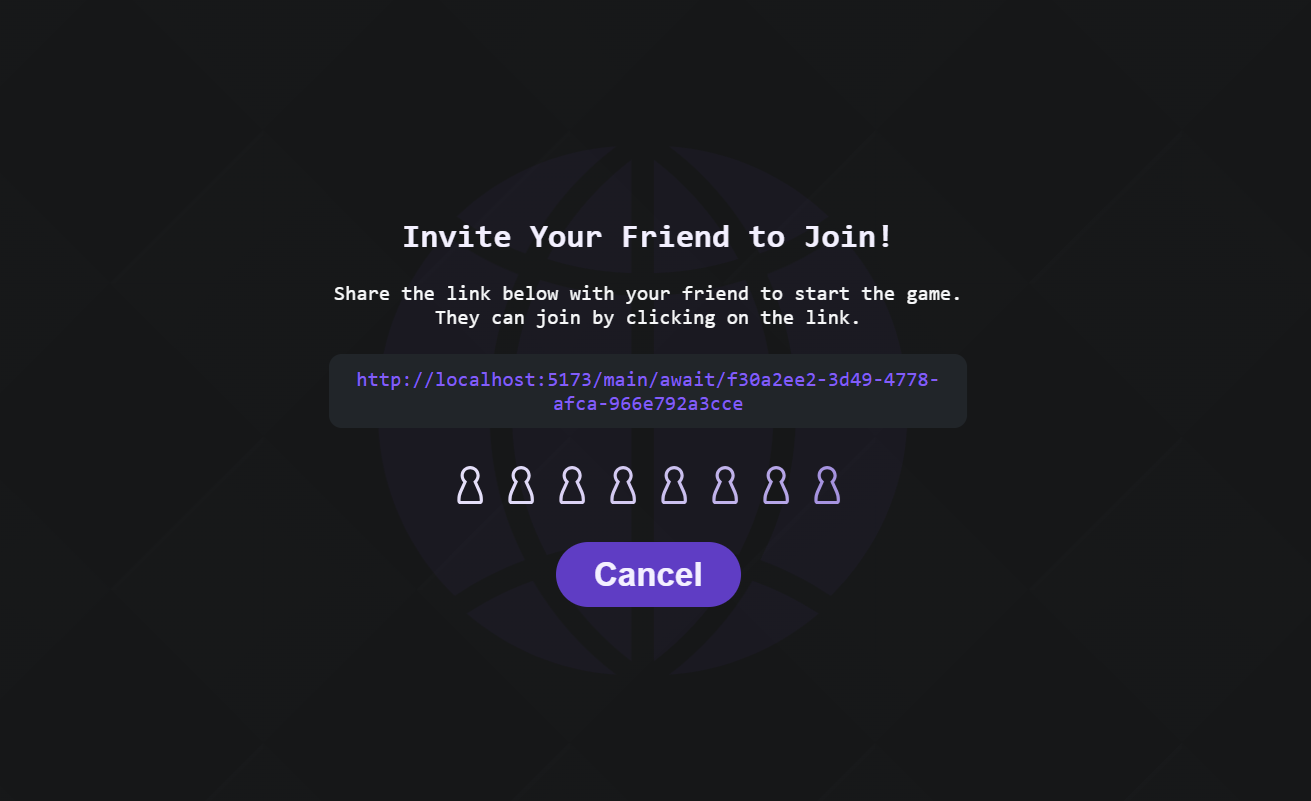
\includegraphics[width=1\textwidth]{zdj/ins_min_link.png}
    \caption{Widok rozpoczynania gry przez link.}
\end{figure}

\newpage
\subsection{Gry użytkownika}
Po kliknięciu na przyciski wyświetlające gry, użytkownik zostaje przeniesiony do sekcji, w której pojawiają się karty gier. W zależności od wybranego przycisku, wyświetlane są gry w różnych stanach. W sekcji „Wciąż aktywne gry” znajdują się partie, które są w trakcie rozgrywki. Jest to szczególnie użyteczne przy długich czasach gry, gdyż gracze mogą wrócić do nierozgrywanych jeszcze partii, kontynuując je w dowolnym momencie. Sekcja „Zakończone gry” pozwala na przeglądanie gier, które już się zakończyły. Użytkownicy mogą sprawdzić, jak przebiegały rozgrywki, jakie strategie były stosowane i jakie były wyniki. Sekcja „Gry z komputerem” oferuje podobną funkcjonalność, umożliwiając przegląd zakończonych gier przeciwko komputerowemu przeciwnikowi. Dzięki temu gracze mogą łatwo wrócić do swoich partii, analizować je i śledzić postępy w grze. Aby powrocic do gry, użytkownik musi zwyczajnie kliknąć w wybraną kartę.
\\\\
Dodatkowo, we wszystkich tych sekcjach istnieją filtry, które umożliwiają łatwiejsze sortowanie gier. Gracze mogą filtrować partie po różnych kryteriach, takich jak rodzaj kontroli czasowej, co pozwala szybko znaleźć gry o określonym czasie, czy wynik gry, umożliwiając sortowanie na podstawie zwycięstw, porażek lub remisów. Filtry te ułatwiają przeglądanie dużej liczby gier, pomagając użytkownikom szybko odnaleźć interesujące ich rozgrywki i dostosować widok do swoich potrzeb.


\begin{figure}[h!]
    \centering
    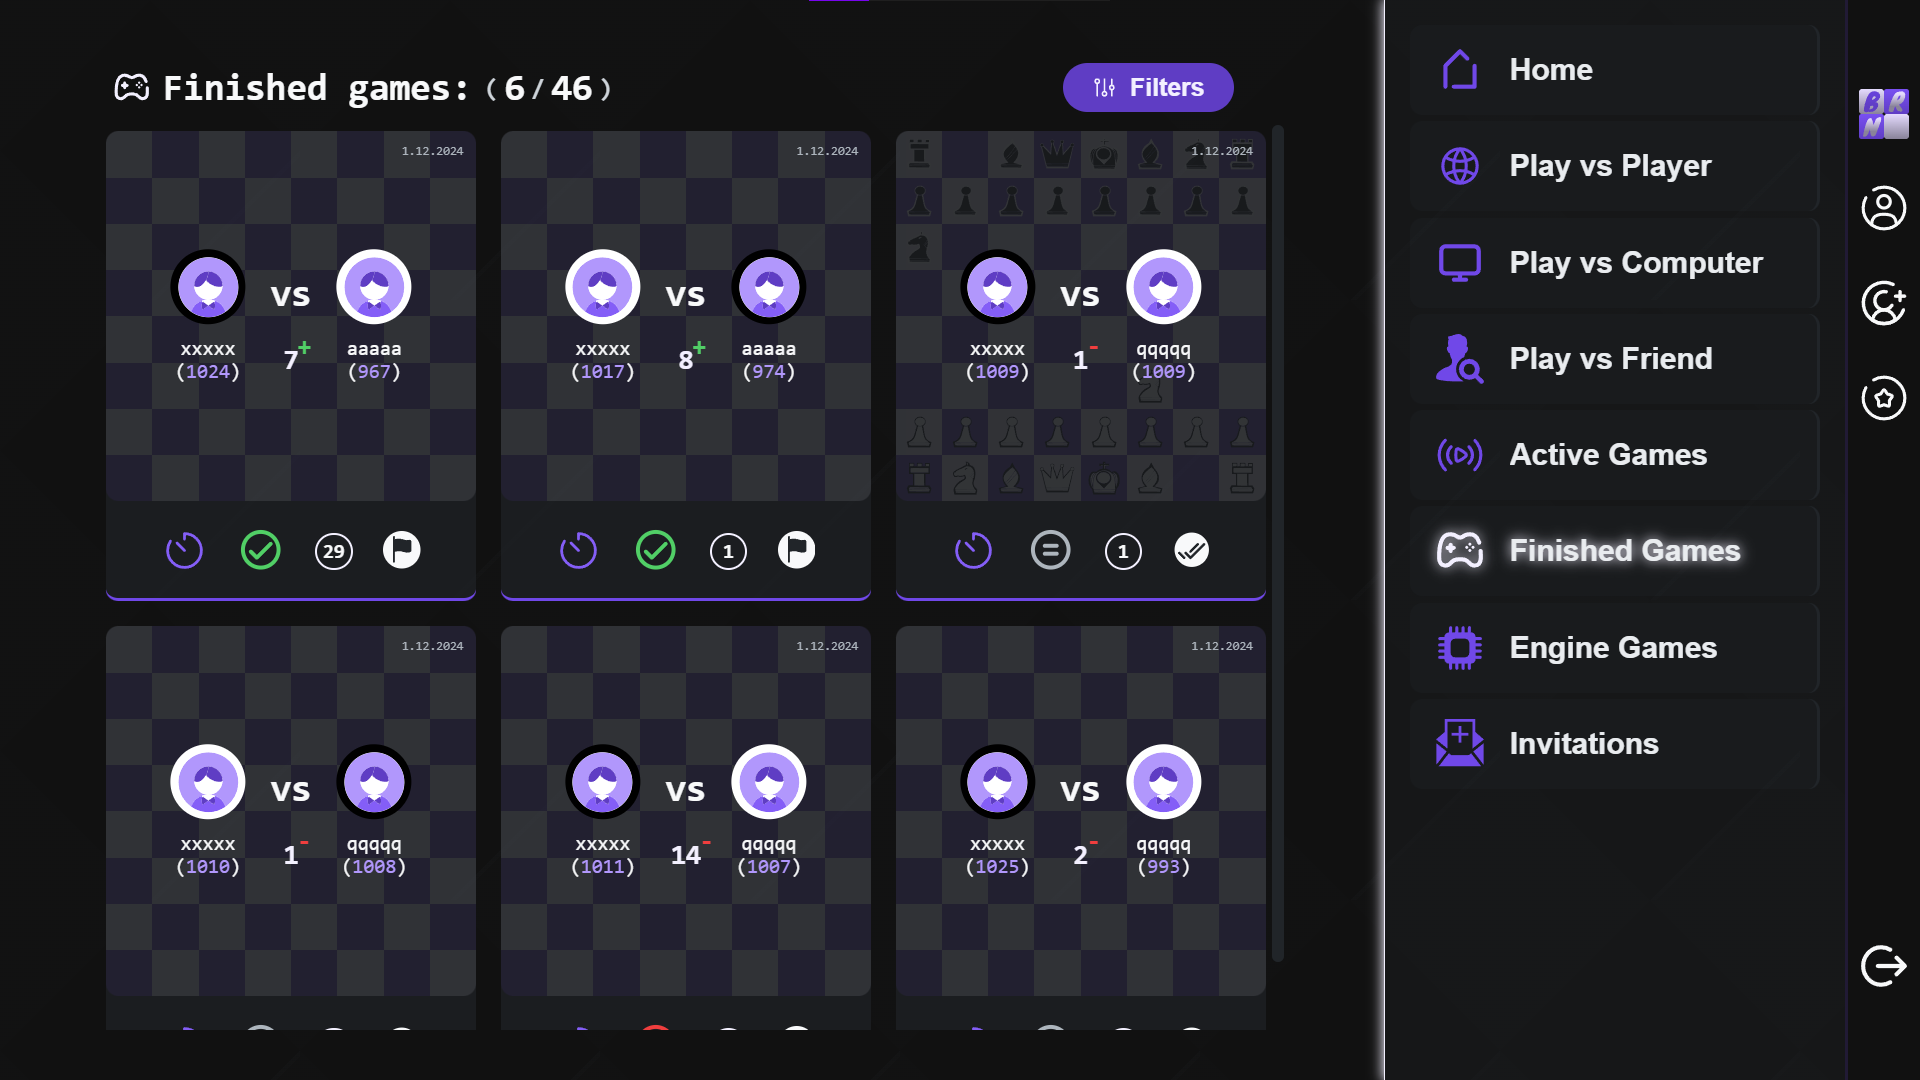
\includegraphics[width=1\textwidth]{zdj/ins_min_games.png}
    \caption{Widok gier użytkownika.}
\end{figure}

\newpage
\subsection{Zaproszenia}
Ostatnia sekcja na głównej stronie to zaproszenia, gdzie użytkownik ma wgląd we wszystkie aktywne zaproszenia do gry. Zaproszenia te mają określony czas ważności – wygasają po 15 minutach, po czym przestają być widoczne. Dzięki temu użytkownicy mają tylko ograniczony czas na przyjęcie zaproszenia, co wprowadza element dynamiki i pilności w interakcje z innymi graczami.

\begin{figure}[h!]
    \centering
    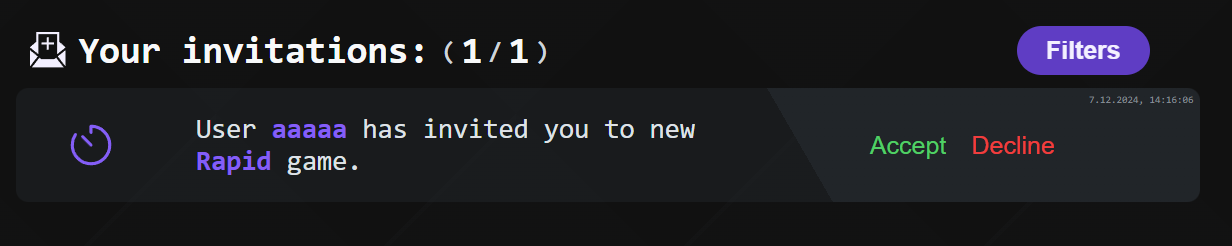
\includegraphics[width=1\textwidth]{zdj/ins_min_inv_card.png}
    \caption{Widok zaproszeń do gry.}
\end{figure}

Dodatkowo, w przypadku gdy użytkownik jest aktywny na stronie, pojawia się specjalnie dedykowane okno popup. Jeśli użytkownik otrzyma zaproszenie do gry, komunikat wyświetli się automatycznie, informując o tym fakcie. W popupie znajdują się również opcje akceptacji lub odrzucenia zaproszenia, co umożliwia szybkie podjęcie decyzji o dołączeniu do gry lub jej odrzuceniu. Dzięki tej funkcji użytkownicy są na bieżąco informowani o zaproszeniach, co ułatwia interakcję i organizowanie rozgrywek. Użytkownik także może użyć filtrów, aby wyświetli już nieaktywne zaproszenia.

\begin{figure}[h!]
    \centering
    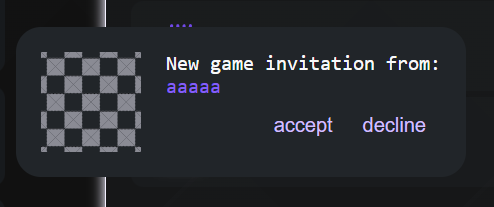
\includegraphics[width=0.7\textwidth]{zdj/ins_min_inv_popup.png}
    \caption{Wyskakujące okienko otrzymanego zaproszenia.}
\end{figure}

\newpage
\subsection{Strona gry}
Na stronie gry, w centralnej części, znajduje się szachownica, która stanowi główny element interfejsu. To tutaj odbywa się sama rozgrywka, a użytkownicy wykonują swoje ruchy. Po obu stronach szachownicy znajdują się panele, które oferują dodatkowe opcje i funkcjonalności, zapewniając pełniejszą kontrolę nad grą i umożliwiając dostęp do różnych narzędzi pomocniczych.

\begin{figure}[h!]
    \centering
    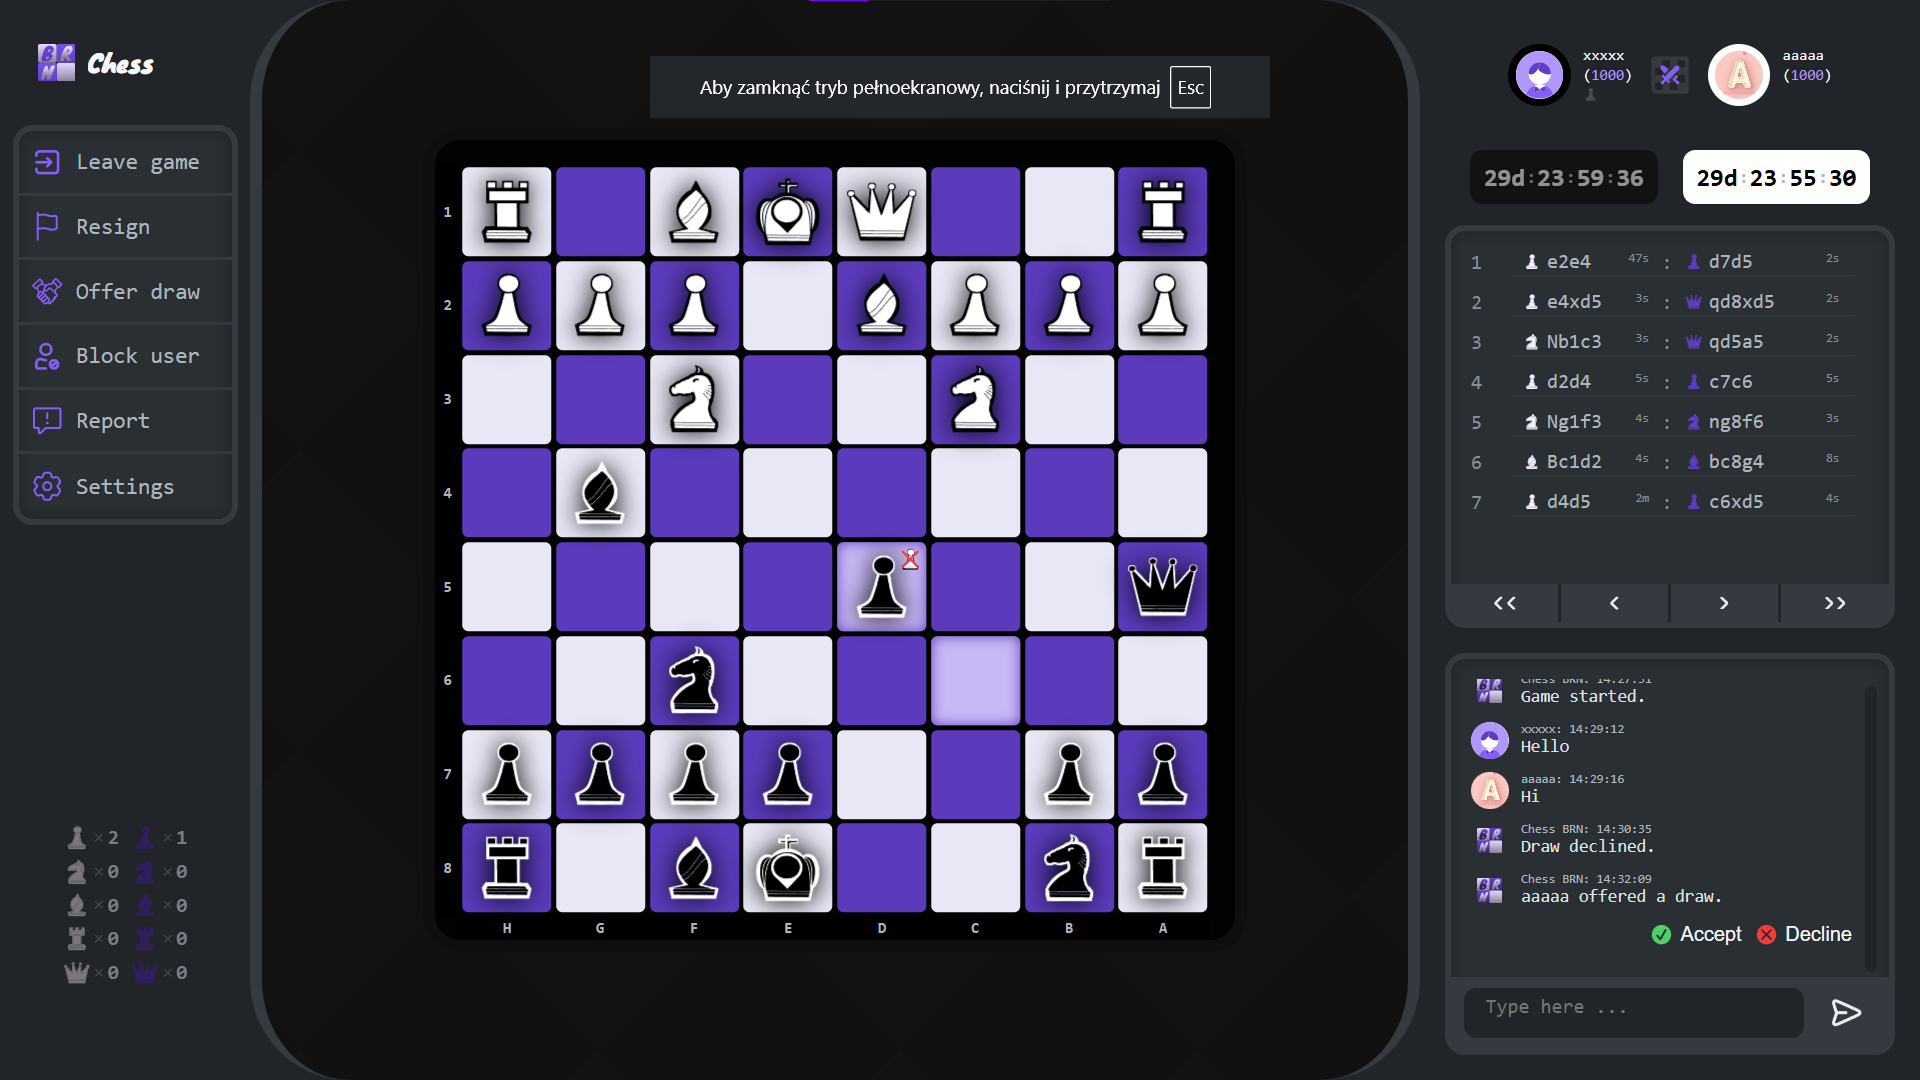
\includegraphics[width=0.9\textwidth]{zdj/ins_webgame.png}
    \caption{Strona gry online.}
\end{figure}

\begin{figure}[h!]
    \centering
    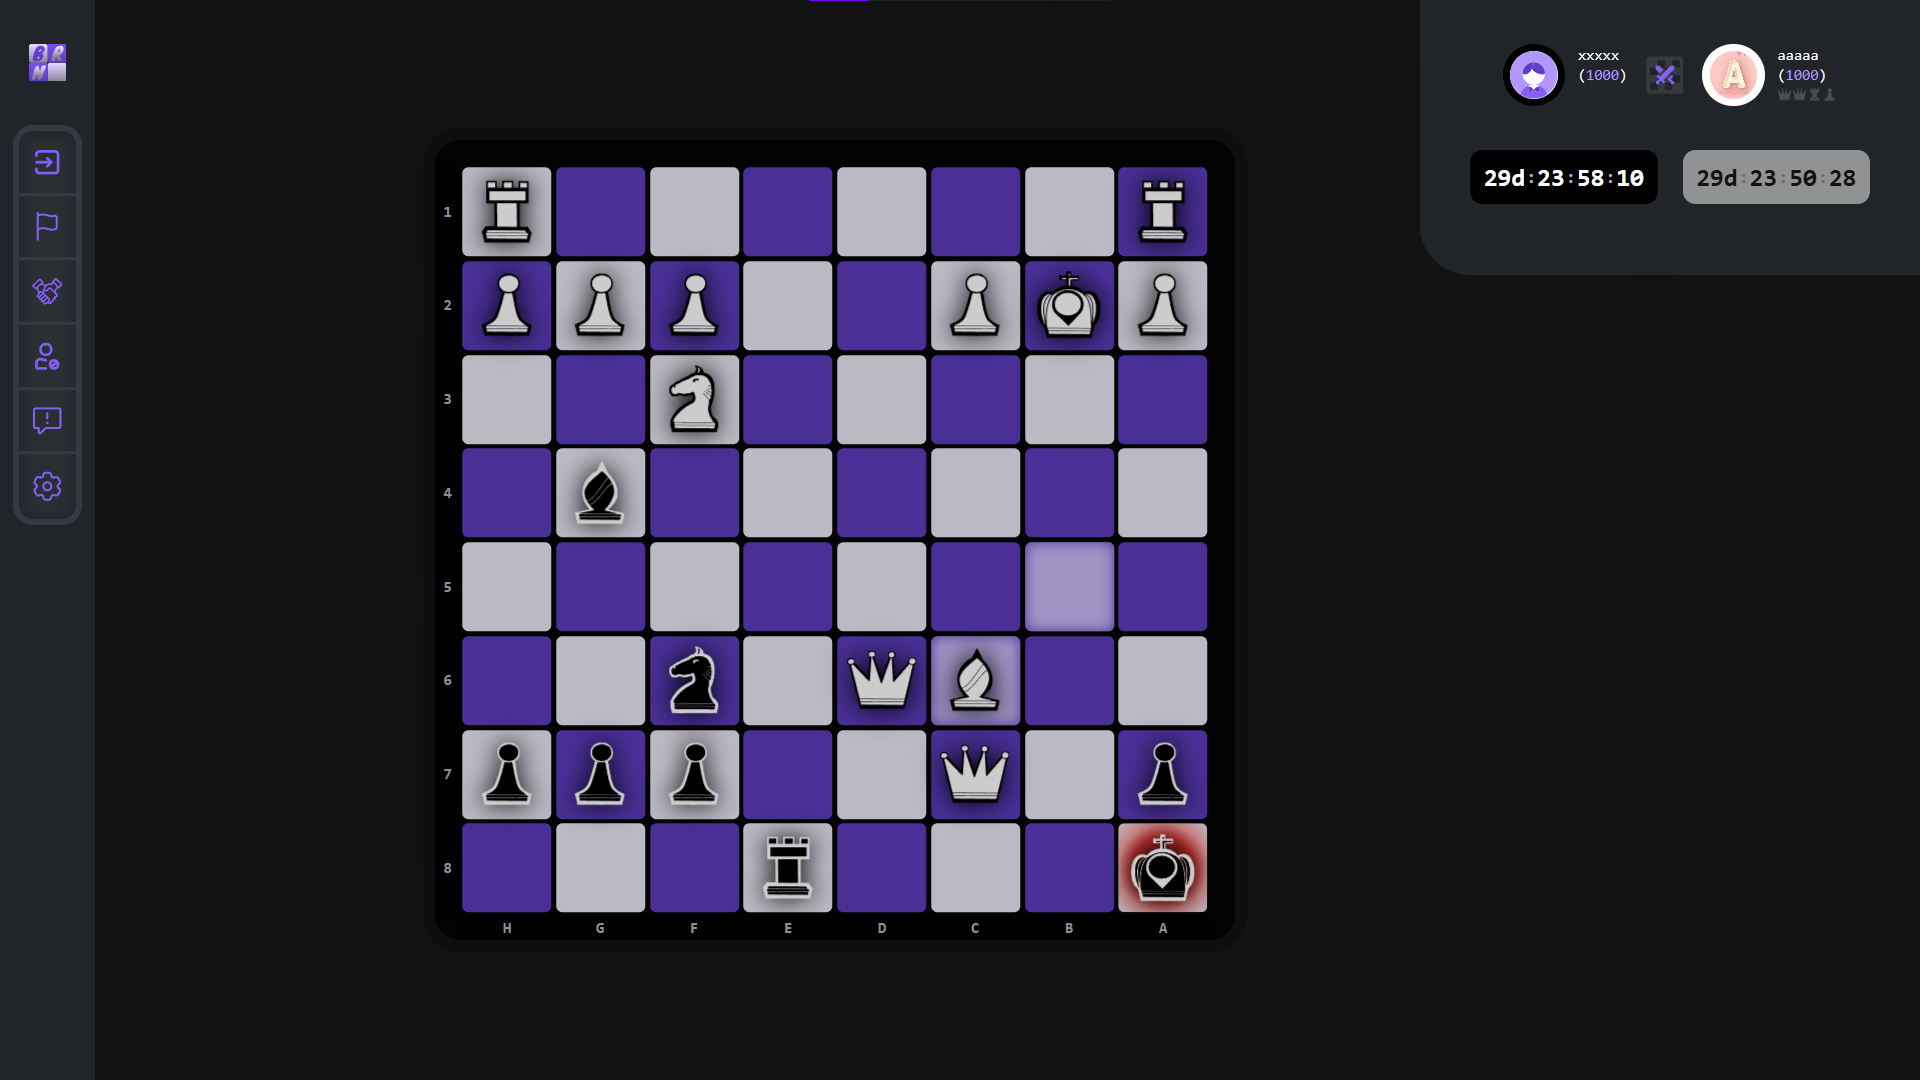
\includegraphics[width=0.9\textwidth]{zdj/ins_simpgame.png}
    \caption{Uproszony widok gry.}
\end{figure}

\newpage

W centralnej części ekranu znajduje się szachownica, której wygląd może być spersonalizowany przez użytkownika w ustawieniach. Po bokach planszy wyświetlane są koordynaty pól (oznaczone literami i cyframi), które pomagają w orientacji na szachownicy. Gracze mogą wybierać i wykonywać ruchy zarówno poprzez kliknięcia, jak i metodę drag and drop, przeciągając figury na odpowiednie pola. Po wykonaniu ruchu przez przeciwnika, odpowiednie pole zostaje podświetlone, co ułatwia śledzenie zmian na planszy. W przypadku zbicia figury, na polu, na którym nastąpiło zbicie, pojawia się mała przekreślona ikona, sygnalizująca utratę figury. Gdy król znajduje się w szachu, jego figura zostaje podświetlona na czerwono, co wskazuje na zagrożenie i konieczność podjęcia działań w celu ochrony króla.

\begin{figure}[h!]
    \centering
    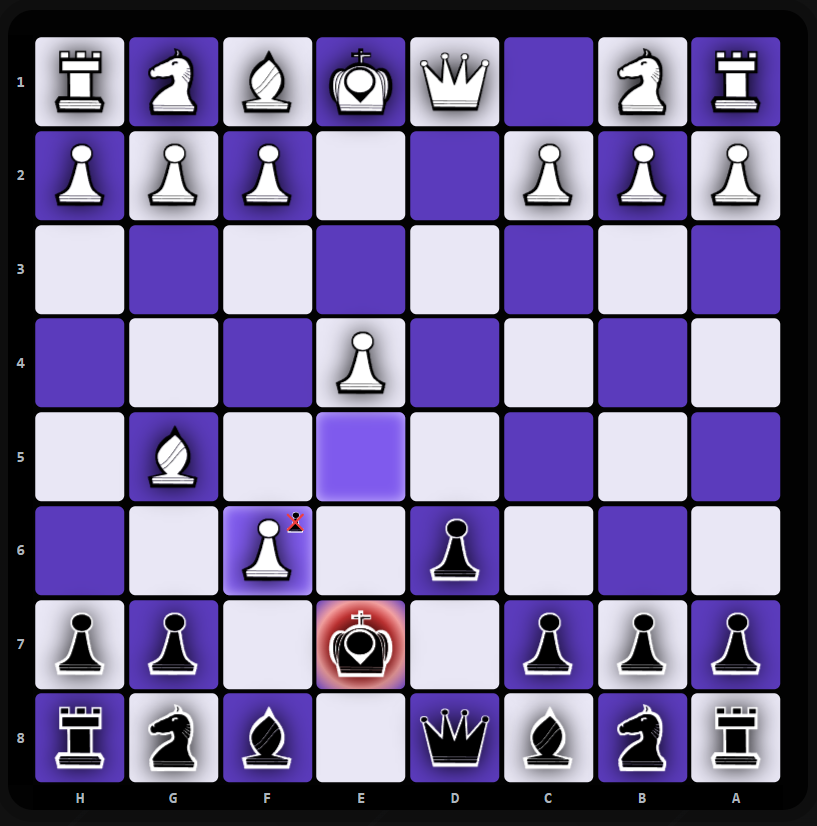
\includegraphics[width=0.9\textwidth]{zdj/ins_min_board.png}
    \caption{Szachownica}
\end{figure}

\newpage


\begin{minipage}[t]{0.45\textwidth} 
    \vspace{0pt} 
    \raggedright 
    Na prawym pasku widnieje informacja o graczach. Pokazuje ich aktualną punktację ELO oraz przewagę materialną w grze, przeliczoną na figury. Dodatkow zaraz poniżej znajduję się czas jaki pozostał każdemu z graczy, istniejący tylko w grach online (nie istnieje podczas gier z silnikiem).
\end{minipage} 
\hfill 
\begin{minipage}[t]{0.45\textwidth} 
    \vspace{0pt} 
    \centering 
    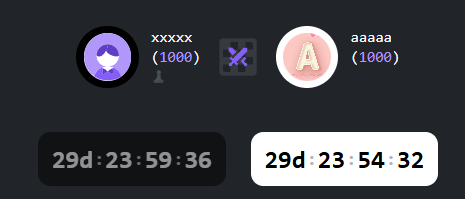
\includegraphics[width=\linewidth]{zdj/ins_min_players.png} 
\end{minipage}

\vspace{1cm}

\begin{minipage}[t]{0.45\textwidth} 
    \vspace{0pt} 
    \centering 
    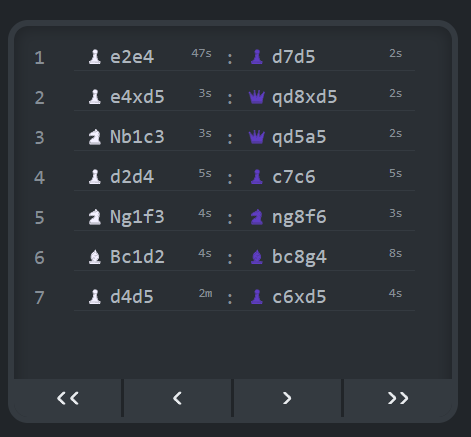
\includegraphics[width=\linewidth]{zdj/ins_min_moves.png} 
\end{minipage} 
\hfill 
\begin{minipage}[t]{0.45\textwidth} 
    \vspace{0pt} 
    \raggedright 
    Kolejna funkcjonalność to menu ruchów, które zostały wykonane. Każdy ruch jest pokazany z ikoną figury, która została użyta, notacją FEN opisującą ruch oraz przybliżonym czasem wykonania ruchu. Na dole menu znajdują się strzałki umożliwiające przewijanie i cofanie, co pozwala na szybki podgląd poprzednich pozycji i śledzenie przebiegu partii. Dodatkowo, najeżdżając na konkretny ruch, wyświetla się wizualizacja pozycji po wykonaniu tego ruchu. Po zakończeniu partii pojawia się przycisk umożliwiający animację całej gry, pozwalając na jej odtworzenie od początku do końca.
\end{minipage}

\vspace{1cm}

\begin{minipage}[t]{0.45\textwidth} 
    \vspace{0pt} 
    \raggedright 
    Ostatnia funkcjonalność na prawym pasku to menu wiadomości. Wyświetlane są tam wiadomości wysłane przez użytkowników, jak również automatyczne powiadomienia, takie jak informacje o rozpoczęciu/zakończeniu gry czy oferta remisu. Na dole menu znajduje się pole do wysyłania własnych wiadomości, co umożliwia graczom łatwą komunikację z innymi uczestnikami gry. W przypadku gry z silnikiem wysłanie wiadomosci jest zablokowane, a wyswietlane sa tylko wiadomosci systemowe.
\end{minipage} 
\hfill 
\begin{minipage}[t]{0.45\textwidth} 
    \vspace{0pt} 
    \centering 
    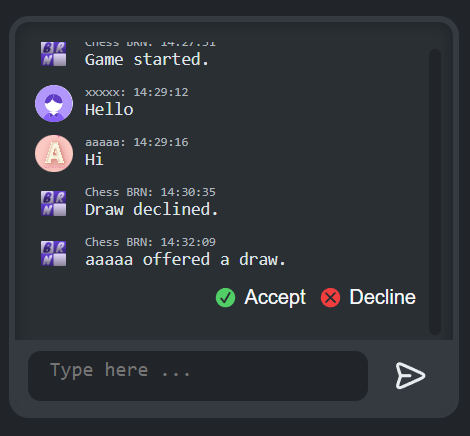
\includegraphics[width=\linewidth]{zdj/ins_min_mess.png} 
\end{minipage}

\newpage

\begin{minipage}[t]{0.2\textwidth} 
    \vspace{0pt} 
    \centering 
    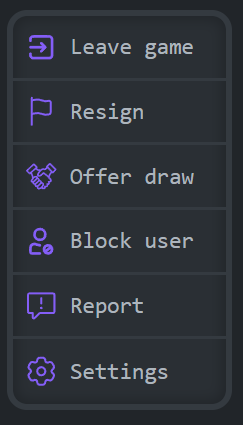
\includegraphics[width=\linewidth]{zdj/ins_min_wopt.png} 
\end{minipage} 
\hfill 
\begin{minipage}[t]{0.7\textwidth} 
    \vspace{0pt} 
    \raggedright 
    Na lewym panelu w przypadku gry online dostępne są opcje zarządzania rozgrywką. Pierwsza z nich to opcja opuszczenia gry, która działa różnie w zależności od długości partii. Dla gier krótkich oznacza to remis, jeśli gra dopiero się rozpoczęła, lub poddanie się, jeśli gra trwa już dłużej. W przypadku gier długich, opuszczenie gry oznacza po prostu wyjście z partii. Kolejna opcja to poddanie się, które kończy grę i uznaje przeciwnika za zwycięzcę. Można również zaproponować remis, co skutkuje wysłaniem oferty do drugiego gracza, który może ją zaakceptować lub odrzucić. Dodatkowo, istnieje opcja blokowania użytkownika, co uniemożliwia wysyłanie wiadomości oraz dodanie takiej osoby do znajomych. Istnieje również możliwość zgłoszenia podejrzenia oszukiwania, co daje użytkownikom narzędzie do zgłaszania nieuczciwych praktyk. Na koniec, dostępne jest ustawienie wyglądu strony gry, w tym zmiana wyglądu szachownicy oraz figur, co pozwala na dostosowanie interfejsu do własnych preferencji.
\end{minipage}

\vspace{1cm}

\begin{minipage}[t]{0.7\textwidth} 
    \vspace{0pt} 
    \raggedright 
    W przypadku gry z silnikiem, lewy panel zawiera nieco inne opcje dostosowane do tego trybu gry. Pierwsza opcja to wyjście z gry, która kończy rozgrywkę. Można również zrestartować grę, co rozpoczyna ją od nowa. Dodatkowo dostępna jest opcja poddania się, kończąca partię na korzyść silnika. Istnieje także możliwość cofnięcia ruchu, ale jest to dostępne tylko wtedy, gdy opcja oszukiwania jest włączona w ustawieniach. Kolejną opcją jest zmiana poziomu silnika, która pozwala na dostosowanie trudności rozgrywki, jednak ta funkcja jest także dostępna tylko przy włączonej opcji oszukiwania. Na koniec, jak w przypadku gry online, dostępna jest opcja zmiany ustawień wyglądu strony gry, w tym szachownicy oraz figur, co pozwala na personalizację wizualną rozgrywki.
\end{minipage} 
\hfill 
\begin{minipage}[t]{0.2\textwidth} 
    \vspace{0pt} 
    \centering 
    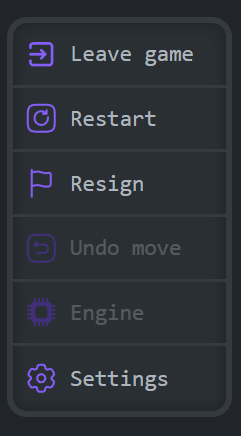
\includegraphics[width=\linewidth]{zdj/ins_min_eopt.png} 
\end{minipage}

\vspace{1cm}

\begin{minipage}[t]{0.2\textwidth} 
    \vspace{0pt} 
    \centering 
    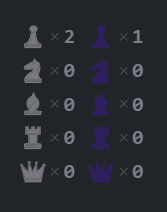
\includegraphics[width=\linewidth]{zdj/ins_min_capt.png} 
\end{minipage} 
\hfill 
\begin{minipage}[t]{0.7\textwidth} 
    \vspace{0pt} 
    \raggedright 
    Ostatnią opcją na lewym panelu jest wyświetlanie zbitych figur. W tej sekcji widoczne są wszystkie figury, które zostały już zbite przez graczy, a obok każdej figury wyświetlana jest liczba, ile ich pozostało. Dzięki temu użytkownicy mogą śledzić, jak przebiega gra pod względem materiału, co pomaga w ocenie pozycji na szachownicy.
\end{minipage}

\newpage
Dodatkowo na planszy szachowej pojawiają się wyskakujące okna, które aktywują się po wybraniu odpowiednich opcji przez użytkownika. Takie okna zwykle służą do potwierdzenia wykonania konkretnej akcji, na przykład w przypadku chęci poddania się, opuszczenia gry czy zmiany ustawień. Wyskakujące okno zawiera pytanie, czy użytkownik na pewno chce wykonać daną czynność, a także opcje potwierdzenia lub anulowania decyzji. Dzięki temu gracze mają pewność, że nie dokonają niezamierzonych zmian czy działań.

\begin{minipage}[t]{0.45\textwidth} 
    \vspace{0pt} 
    \centering 
    Okno promocji pionka pojawia się, gdy pionek dotrze do ostatniej linii. Użytkownik wybiera jedną z czterech opcji: damę, wieżę, skoczka lub gońca, a pionek zostaje zamieniony na wybraną figurę.
\end{minipage} 
\hfill 
\begin{minipage}[t]{0.45\textwidth} 
    \vspace{0pt} 
    \centering 
    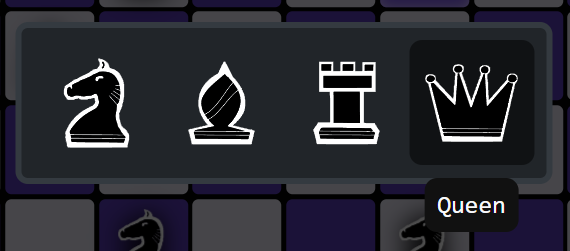
\includegraphics[width=\linewidth]{zdj/ins_min_prom.png} 
\end{minipage}

\vspace{1cm}

\begin{minipage}[t]{0.45\textwidth} 
    \vspace{0pt} 
    \centering 
    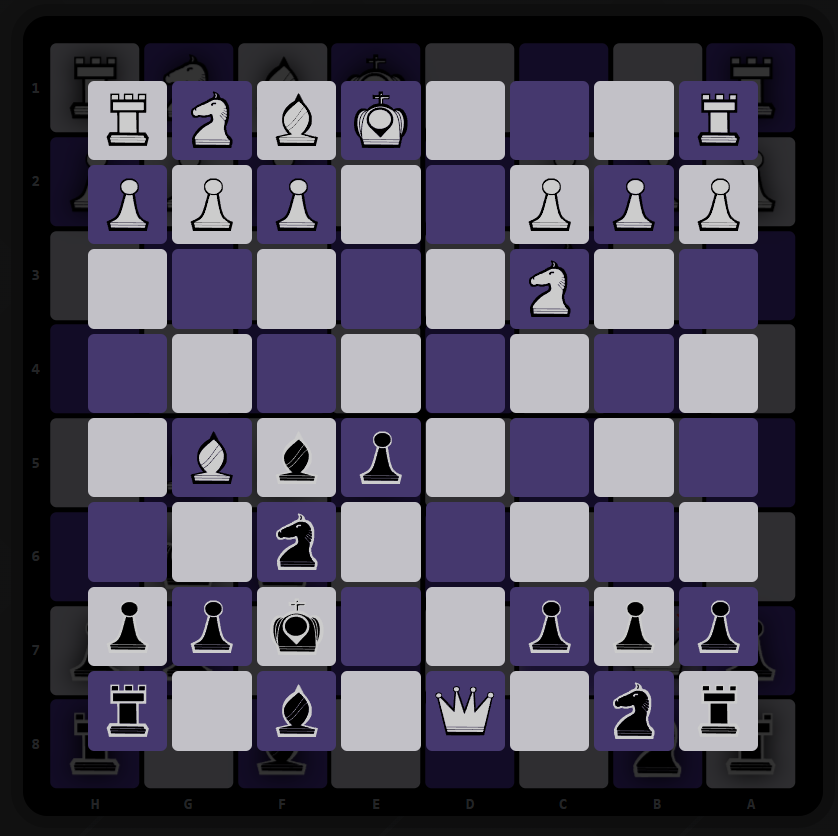
\includegraphics[width=\linewidth]{zdj/ins_min_prev.png} 
\end{minipage} 
\hfill 
\begin{minipage}[t]{0.45\textwidth} 
    \vspace{40pt}
    \centering 
    Pokazywanie poprzednich ruchów odbywa się po najechaniu myszką na menu z poprzednimi ruchami. Po wybraniu ruchu, na szachownicy pojawia się pomniejsza, przyciemniona plansza, która pokazuje wcześniejszą pozycję. Ta zmiana jest tylko wizualna, nie można nic zrobić na tej pomniejszonej planszy, służy ona jedynie do pokazania poprzedniego stanu gry.
\end{minipage}


\vspace{1cm}

\begin{minipage}[t]{0.45\textwidth} 
    \vspace{0pt} 
    \centering 
    Innym wyskakującym oknem jest okno, które pojawia się po zakończeniu gry, niezależnie od wyniku — wygranej, przegranej lub remisie. Na tym oknie wyświetlany jest rezultat gry, czyli informacja, kto wygrał, jaki był powód zakończenia gry oraz punkty zdobyte lub stracone przez graczy. Na dole okna znajdują się przyciski umożliwiające przejście do wyjścia z gry, rozpoczęcia nowej partii lub rozegrania rewanżu, przy czym będą one odbywać z dotychczasową kontrolą czasową. W przypadku gier z silnikiem dostępne są jedynie opcje restartu gry lub wyjścia z gry.
\end{minipage} 
\hfill 
\begin{minipage}[t]{0.45\textwidth} 
    \vspace{0pt} 
    \centering 
    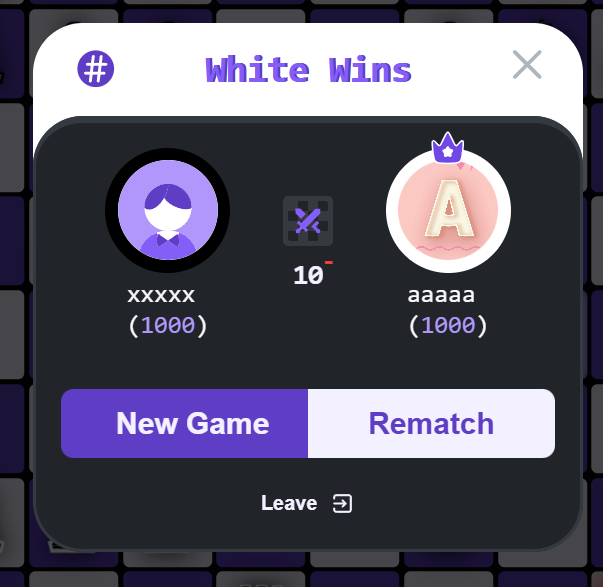
\includegraphics[width=\linewidth]{zdj/ins_min_win.png} 
\end{minipage}

\newpage
\subsection{Strona profilu}
Strona profilu użytkownika zapewnia pełną kontrolę nad ustawieniami konta oraz personalizacją preferencji. Użytkownik ma możliwość edytowania swojego profilu, w tym zmiany danych osobowych, zdjęcia profilowego oraz innych informacji. Na stronie dostępne są szczegółowe statystyki gier, w tym wykresy punktacji dla różnych kategorii czasowych, które pozwalają na analizowanie postępów i wyników w różnych wariantach gier. Użytkownik może również przeglądać listę swoich znajomych, zapraszać ich do gry oraz oglądać ich profile.
\\\\
Dodatkowo, użytkownik ma możliwość edytowania ustawień konta, w tym zmiany hasła oraz zarządzania ustawieniami prywatności, takimi jak widoczność profilu. Można również dostosować wygląd strony gry, zmieniając szachownicę, pionki oraz inne elementy wizualne. Istnieje opcja włączenia funkcji oszukiwania podczas gry z silnikiem, co pozwala na cofanie ruchów lub zmianę poziomu trudności. Ponadto, użytkownik może zarządzać globalnymi ustawieniami aplikacji, takimi jak język czy powiadomienia. Strona profilu jest centralnym miejscem, w którym użytkownik może zarządzać wszystkimi aspektami swojego konta i dostosować aplikację do swoich potrzeb.

\begin{figure}[h!]
    \centering
    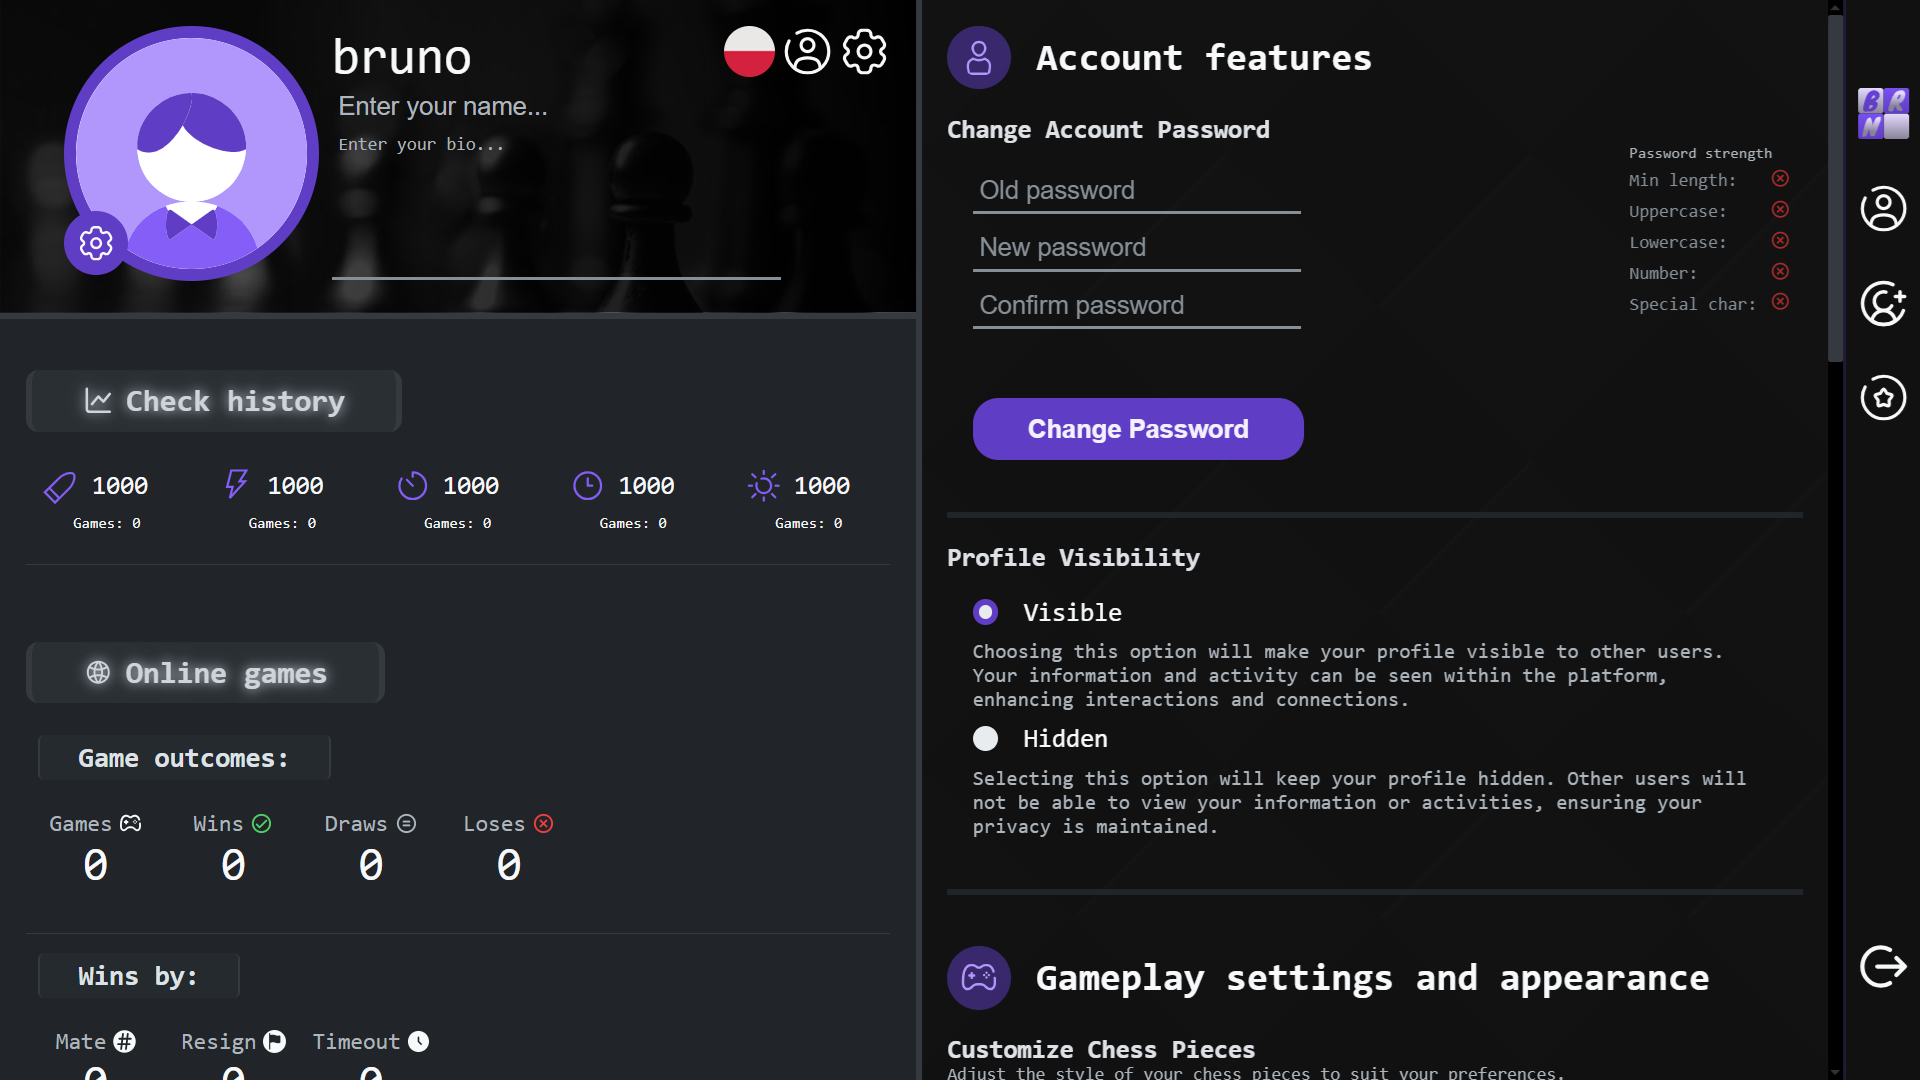
\includegraphics[width=1\textwidth]{zdj/ins_account.png}
    \caption{Strona profilu użytkownika.}
\end{figure}

\newpage
\subsection{Strona zarządzania znajomymi}
Strona użytkowników służy do zarządzania znajomymi i relacjami z innymi graczami w aplikacji. Jest podzielona na cztery główne sekcje, które pomagają w organizowaniu kontaktów.

\begin{itemize}
    \item \textbf{Wszyscy użytkownicy} – zawiera listę wszystkich graczy dostępnych w aplikacji. Z tej sekcji użytkownicy mogą zapraszać innych do znajomych oraz podglądać ich mini profile.
    
    \item \textbf{Twoi znajomi} – znajdują się tutaj osoby, które zostały już dodane do listy znajomych. Można stąd zapraszać znajomych do gry lub przejść do pełnego profilu danego użytkownika.
    
    \item \textbf{Oczekujące zaproszenia} – sekcja zawiera zaproszenia, które zostały wysłane, ale jeszcze nie zostały zaakceptowane przez drugą stronę. Użytkownicy mogą tu zobaczyć zarówno wysłane zaproszenia, jak i te, które czekają na odpowiedź.
    
    \item \textbf{Odrzucone zaproszenia} – lista osób, które odrzuciły zaproszenia do znajomych. Użytkownicy mają możliwość ponownego wysłania zaproszenia do tych osób, jeżeli zechcą.
\end{itemize}

Cała strona umożliwia łatwe zarządzanie znajomymi, zaproszeniami i relacjami z innymi graczami, co pozwala na lepszą organizację kontaktów w aplikacji.

\begin{figure}[h!]
    \centering
    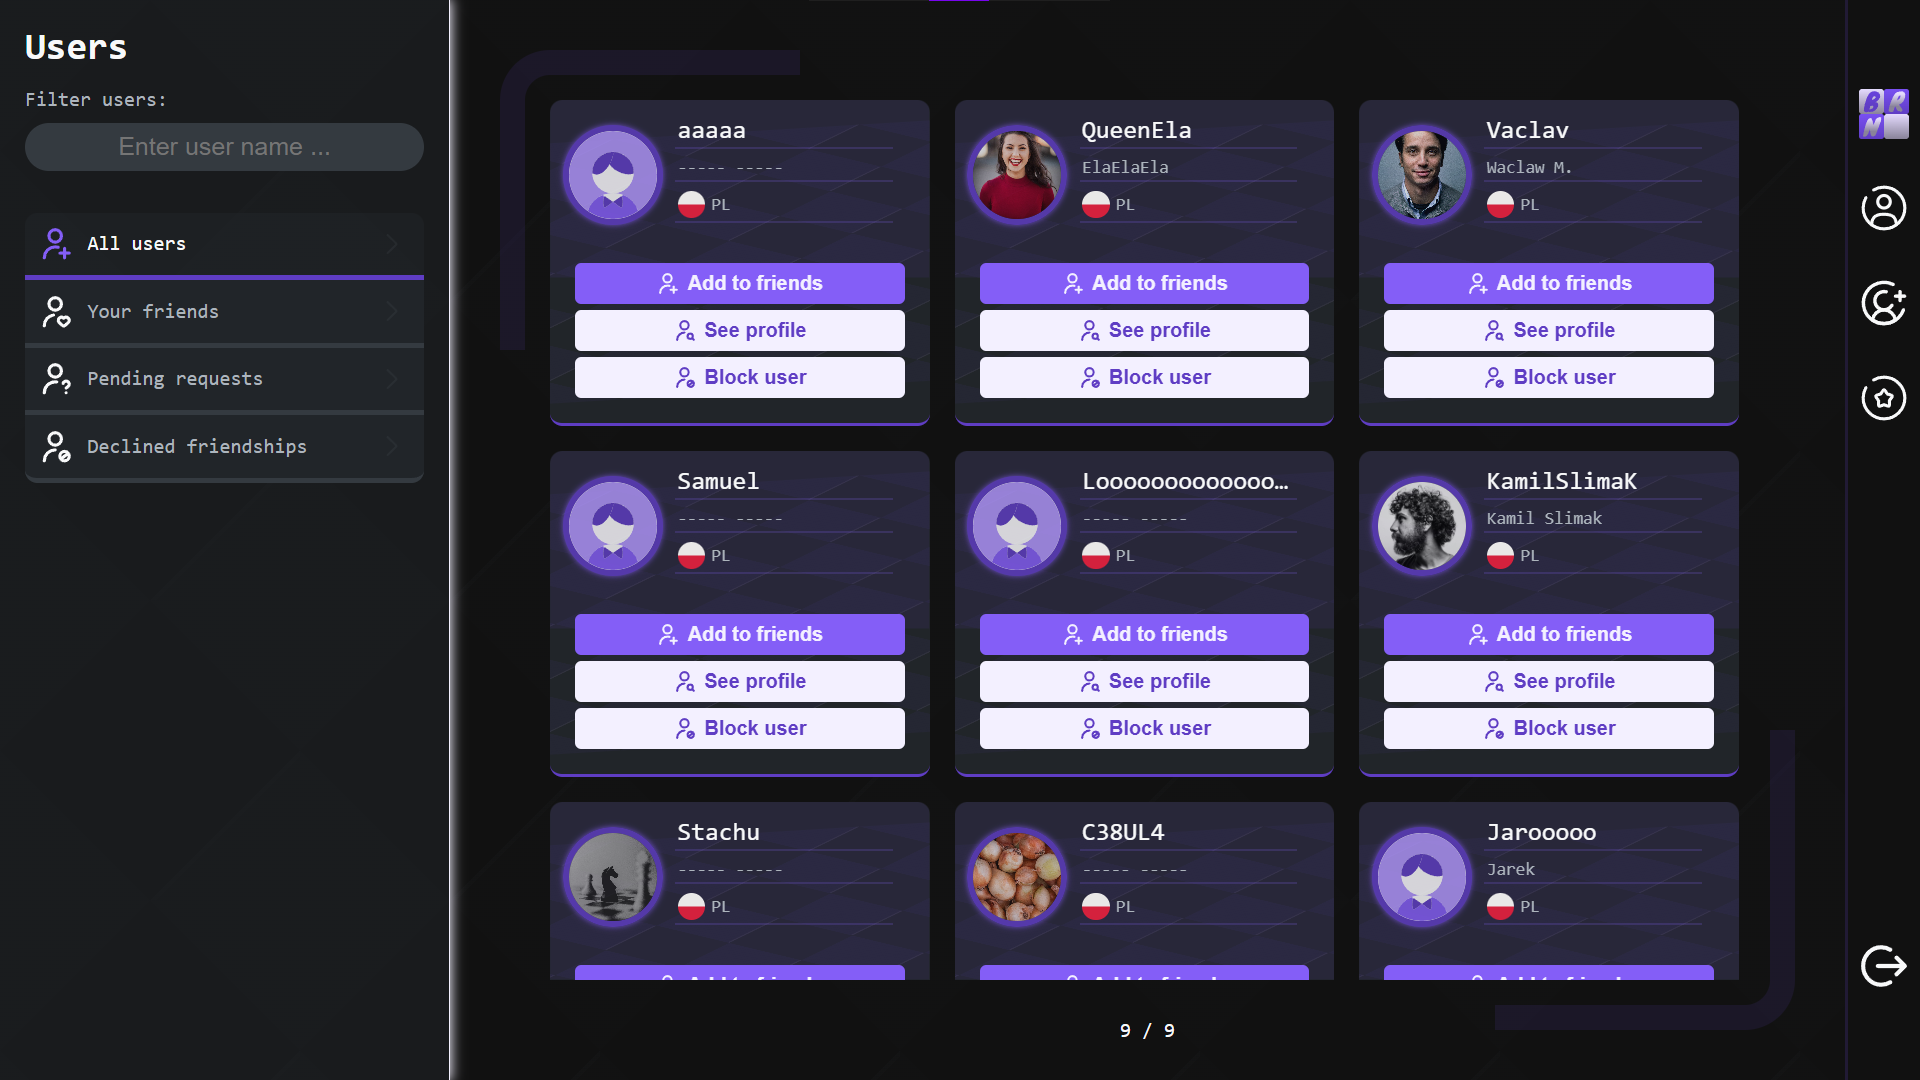
\includegraphics[width=1\textwidth]{zdj/ins_users.png}
    \caption{Strona zarządzania znajomymi.}
\end{figure}

\newpage

\subsection{Strona rankingu}
Strona rankingu pozwala użytkownikom na sprawdzenie ich pozycji w hierarchii graczy aplikacji. Gracze mogą wybierać między dwoma głównymi opcjami: globalnym rankingiem, który obejmuje wszystkich zarejestrowanych użytkowników aplikacji, oraz rankingiem wśród znajomych, który ogranicza wyświetlane wyniki do osób dodanych do listy znajomych.
\\\\
Dodatkowo rankingi są podzielone na pięć kategorii, zależnie od typu kontroli czasowej: bullet, blitz, rapid, classic oraz daily. Dzięki temu gracze mają możliwość sprawdzenia swoich wyników i miejsca w rankingu w kontekście preferowanego rodzaju gry, zarówno na poziomie globalnym, jak i w gronie znajomych.
\\\\
Strona rankingu jest kluczowym elementem aplikacji, wspierającym rywalizację i pozwalającym graczom śledzić ich postępy oraz porównywać swoje osiągnięcia z innymi użytkownikami.

\begin{figure}[h!]
    \centering
    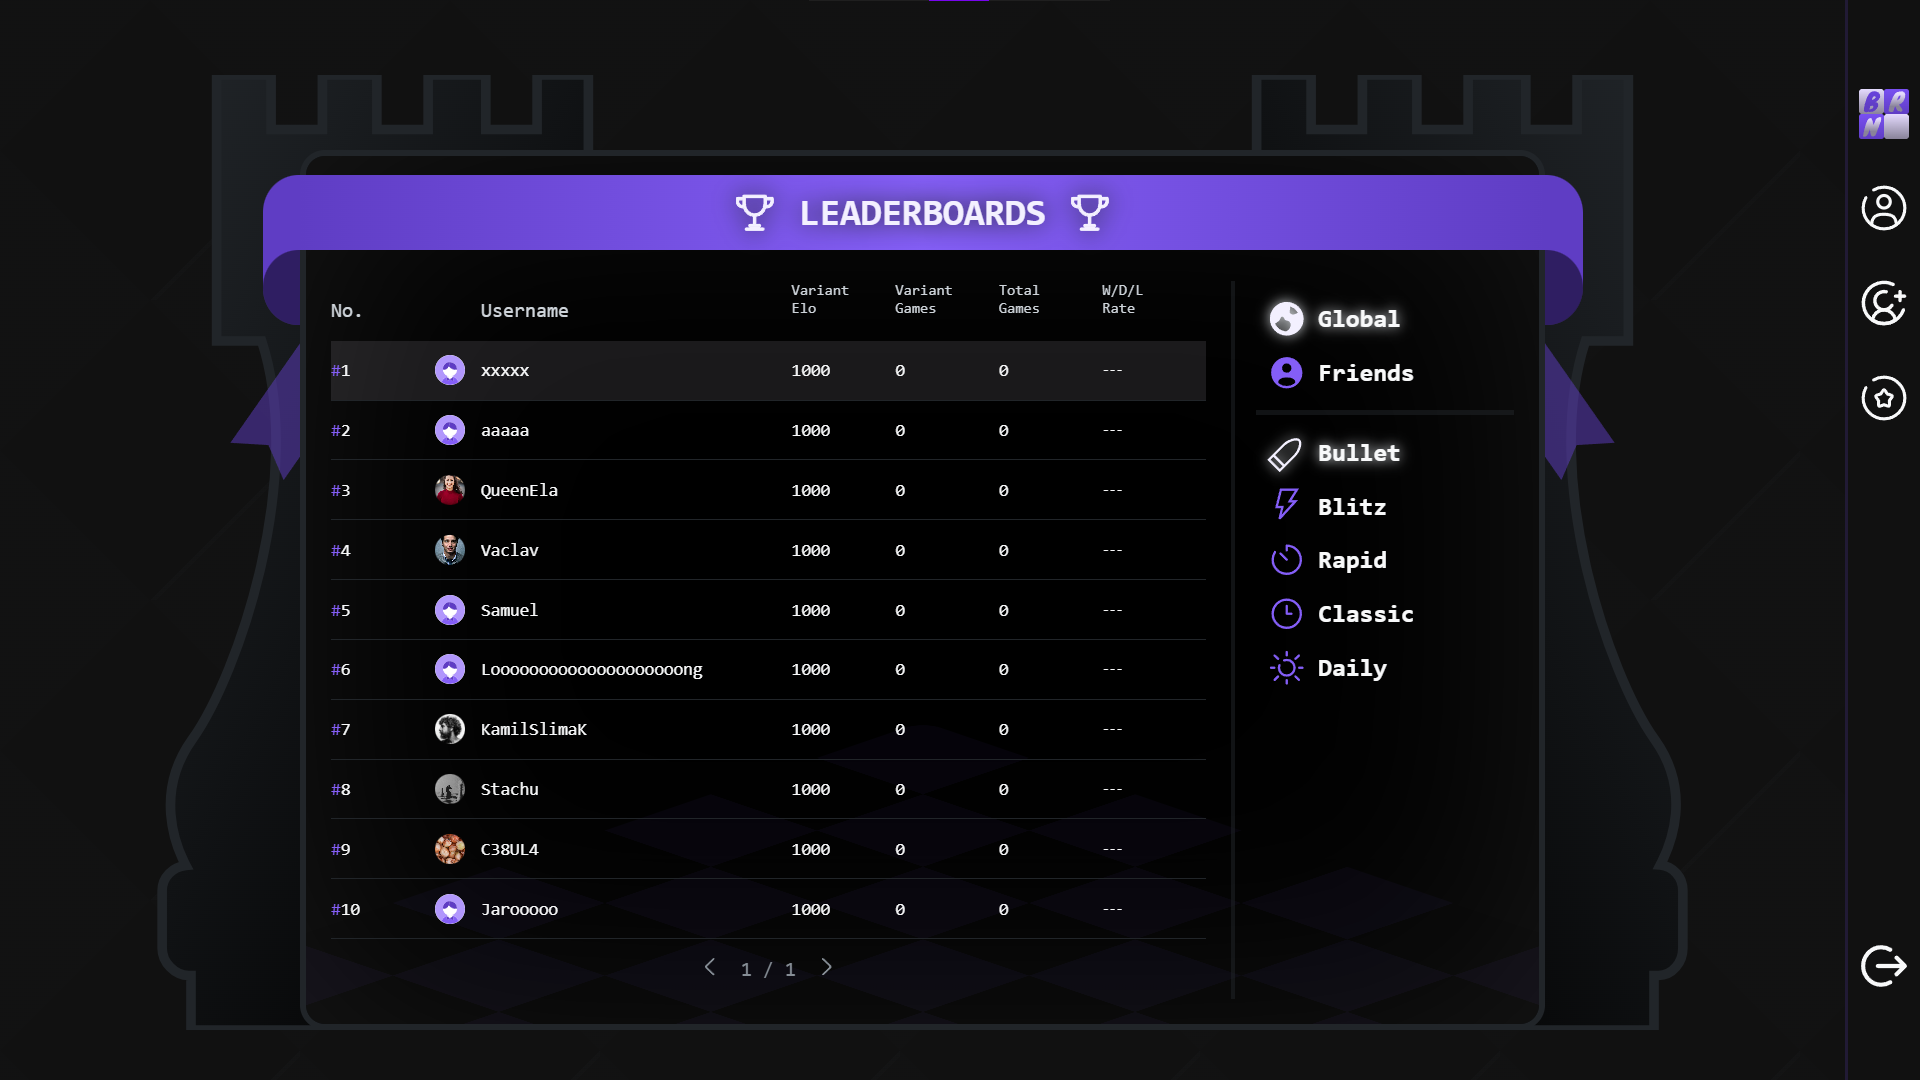
\includegraphics[width=1\textwidth]{zdj/ins_rank.png}
    \caption{Strona zarządzania znajomymi.}
\end{figure}

\newpage
\section{Testy}
\subsection{Frontend}
\subsubsection{Testy automatyczne}
\subsubsection{Testy maunalne}

\newpage
\subsection{Backend}
\subsubsection{Testy jednostkowe}
Test jednostkowy to kod wykonujący inny kod w kontrolowanych warunkach w ramach jednego procesu w pamięci, w celu weryfikacji (bez ingerencji programisty), że testowana logika działa w ściśle określony sposób.
\\\\
W niniejszym projekcie testy jednostkowe zostały wykorzystane w celu automatycznej kontroli poprawności działania klas obsługującym otrzymane zapytania (RequestHandler). Do każdego przypadku obsługi został utworzony test, sprawdzający zarówno poprawną realizację procedury oraz kazdy z możliwych i zaimplementowanych opcji niepoprawnego zapytania.
\\\\


\subsubsection{Testy integracyjne}
Testy integracyjne to etap w procesie tworzenia oprogramowania, który polega na łączeniu i sprawdzaniu, jak ze sobą współpracują różne części systemu. Mają na celu identyfikację potencjalnych błędów i niezgodności, które mogą pojawić się podczas interakcji między różnymi modułami. Zaczynając, należy pamiętać, że osiągniecie powodzenia w testach integracyjnych wymaga zrozumienia całej struktury systemu, jak również umiejętności identyfikacji kluczowych punktów interakcji. Jest to proces wymagający, ale dający wartościowe informacje powiązane z ogólnym działaniem aplikacji.
\\\\


\newpage
\section{Podsumowanie}

\newpage
\section{Literatura}

\begin{itemize}
    \item https://react.dev/learn/describing-the-ui
    \item https://vitejs.dev/guide/
    \item https://en.wikipedia.org/wiki/Chess
    \item https://boringowl.io/blog/testy-integracyjne-plusy-i-minusy-ich-stosowania
    \item https://devstyle.pl/2020/06/25/mega-pigula-wiedzy-o-testach-jednostkowych/
    \item https://boringowl.io/tag/figma
    \item https://justjoin.it/blog/wszystko-co-musicie-wiedziec-o-javascript-co-to-dla-kogo-i-ile-zarobimy
    \item https://www.droptica.pl/blog/co-jest-typescript-i-dlaczego-sprawdzi-sie-w-twoich-projektach/
    \item https://boringowl.io/blog/przeglad-vitejs-nowa-generacja-narzedzi-do-budowania-aplikacji-front-end
    \item https://boringowl.io/blog/poznaj-sass-zyskaj-kontrole-nad-stylem-swojej-strony
    \item https://blog.strefakursow.pl/jezyk-c-czym-jest-i-gdzie-sie-go-uzywa/
    \item https://learn.microsoft.com/pl-pl/dotnet/framework/get-started/
    \item https://www.ovhcloud.com/pl/learn/what-is-postgresql/
    \item https://learn.microsoft.com/pl-pl/devops/develop/git/what-is-git
    \item https://coderslab.pl/pl/blog/github-co-to-jest-i-do-czego-sluzy
    \item https://polontech.com/pl/sourcetree/
    \item https://www.droptica.pl/blog/co-jest-postman-do-czego-sluzy-i-jakie-sa-jego-funkcjonalnosci/
    \item https://www.ovhcloud.com/pl/learn/what-is-rest-api/
\end{itemize}

\end{document}
